\section{Linear dynamical system}\label{chapter-05:section:linear-dynamical-system}

As a first example, we will explore a Bayesian inference task in a \ac{lds}. 
\Ac{lds} systems are widely used in various domains, including signal processing
\citep{sarkka_bayesian_2013}, control \citep{pmlr-v134-chen21c}, finance
\citep{Lahmiri_lds_in_finance}, telecommunications \citep{Lawrence_kalman_equalization}, and
others.
An \ac{lds} is an instance of a state-space model that evolves in time $t$, where the next state of
the system depends only on the previous state.
The dependency is linear and is specified by a transition matrix $A$.
By modeling the system's behavior through a transition matrix, an \ac{lds} enables the prediction
of future states and the estimation of unobservable states from observed measurements.
This makes \ac{lds} an invaluable tool for real-time signal processing applications (\hyperlink{experiments:utility}{\emph{Utility}}).

In its general form, an \ac{lds} model can be expressed as follows \begin{equation}
  \label{eq:sim:lds}
  \begin{split} 
    s_t &= A s_{t - 1} + v_{t}, \\% ~~\sigma_{t} \sim \mathcal{N}(0, \Sigma)\\ 
    y_t &= B s_t + w_{t}, %~~\omega_{t} \sim \mathcal{N}(0, \Omega)
  \end{split}
\end{equation} 
where $s_t$ denotes the state of the system at time $t$, $A$ represents the linear state transition
matrix, $y_t$ corresponds to observation at time $t$, $B$ is the observational matrix, $v_t$ and $w_t$ are process and measurement noise signals, respectively.
The stochastic components of an \ac{lds}, $v_{t}$ and $w_{t}$, are often assumed to be
Gaussian distributed with zero mean and covariance matrices $\Sigma$ and $\Omega$,
respectively.
\begin{equation}
    \label{eq:sim:lds-stochastic-gaussian}
    \begin{split}
        v_{t} &\sim \mathcal{N}(0, \Sigma) \\
        w_{t} &\sim \mathcal{N}(0, \Omega) \\
    \end{split}
\end{equation}
With this assumption, by expressing the model in terms of probability densities, we obtain the following model specification:
\begin{equation}
  \label{eq:sim:lds_probabilities}
  \begin{aligned}
    p(s_t\vert s_{t-1}, \Sigma) & = \mathcal{N}(s_t \vert A s_{t-1}, \Sigma) \\ 
    p(y_t\vert s_{t}, \Omega) & = \mathcal{N}(y_t \vert B s_{t}, \Omega)\,.
  \end{aligned}
\end{equation} 
In the first equation, $p(s_t\vert s_{t-1}, \Sigma)$, denotes the conditional distribution of the state $s_t$ given the previous state $s_{t-1}$ and the covariance matrix $\Sigma$.
Similarly, the second equation, $p(y_t\vert s_{t}, \Omega)$, represents the conditional probability distribution 
of the observation $y_t$ given the current state $s_t$ and the covariance matrix $\Omega$.
% These equations illustrate the probabilistic nature of the linear state-space model.

The complete probabilistic model for the observed signal $\bm{y} = (\bm{y}_1,\bm{y}_2,\ldots,\bm{y}_T)$ can be expressed as \begin{equation}
  \label{eq:sim:lds_model}
  p(\bm{y}, \bm{s}, \Sigma, \Omega) =
  \underbrace{p(\Sigma)p(\Omega)p(s_1)}_{\mathrm{prior}}\underbrace{\prod_{t = 1}^{T} p(y_t\vert
    s_t, \Omega)}_{\mathrm{likelihood}}\underbrace{\prod_{t = 2}^{T}p(s_t\vert s_{t - 1},
    \Sigma)}_{\mathrm{state~transitions}},
\end{equation} where $p(\Sigma)$,
$p(\Omega)$, and $p(s_1)$ denote the priors for $\Sigma$, $\Omega$, and $s_1$, respectively.
Prior terms contribute to the overall prior probability of the model, incorporating prior
beliefs or knowledge about the covariance matrices and the initial state.
This formulation provides a comprehensive representation of the probabilistic model that
includes prior, likelihoods, and state transitions.
Figure~\eqref{fig:sim:lds_model_graph} provides a visual representation of the probabilistic
model~\eqref{eq:sim:lds_model} in the form of \ac{tffg}.
The \ac{tffg} visualizes the dependencies and flow of information within the model and illustrates
the interconnections between the different components of the \ac{lds} model.

\begin{figure}
  \centering
  \resizebox{\textwidth}{!}{\begin{tikzpicture}
  \node[] (splink) {$\cdots$};
  \node[box, node distance=3mm] (spN) [right=of splink] {$\mathcal{N}$};
  \node[smallbox] (speq) [right=of spN] {\small $=$};
  \node[box, node distance=5mm] (spf) [right=of speq] {$A$};
  \node[box, node distance=5mm] (spfN) [right=of spf] {$\mathcal{N}$};
  \node[box, node distance=3mm] (spg) [below=of speq] {$B$};
  \node[box, node distance=3mm] (spgN) [below=of spg] {$\mathcal{N}$};
  \node[clamped, node distance=5mm] (yp) [below=of spgN] {};

  \path[line] (splink) edge[-] (spN);
  \path[line] (spN) edge[-] node[pos=0.5, anchor=south]{$s_{t - 1}$} (speq);
  \path[line] (speq) edge[-] (spf);
  \path[line] (speq) edge[-] (spg);
  \path[line] (spf) edge[-] (spfN);
  \path[line] (spg) edge[-] node[pos=0.5, anchor=east](spgleft){} node[pos=0.5, anchor=west](spgright){} (spgN);
  \path[line] (spgN) edge[-] node[pos=0.5, anchor=west]{$y_{t - 1}$} (yp);

  \node[smallbox] (seq) [right=of spfN] {\small $=$};
  \node[box, node distance=5mm] (sf) [right=of seq] {$A$};
  \node[box, node distance=5mm] (sfN) [right=of sf] {$\mathcal{N}$};
  \node[box, node distance=3mm] (sg) [below=of seq] {$B$};
  \node[box, node distance=3mm] (sgN) [below=of sg] {$\mathcal{N}$};
  \node[clamped, node distance=5mm] (y) [below=of sgN] {};

  \path[line] (spfN) edge[-] node[pos=0.5, anchor=south]{$s_{t}$} (seq);
  \path[line] (seq) edge[-] (sf);
  \path[line] (seq) edge[-] (sg);
  \path[line] (sf) edge[-] (sfN);
  \path[line] (sg) edge[-] node[pos=0.5, anchor=east](sgleft){} node[pos=0.5, anchor=west](sgright){} (sgN);
  \path[line] (sgN) edge[-] node[pos=0.5, anchor=west]{$y_{t}$} (y);

  \node[] (snlink) [right=of sfN] {$\cdots$};
  \node[box, node distance=5mm] (sTN) [right=of snlink] {$\mathcal{N}$};
  \node[smallbox, draw=white, node distance=5mm] (sTeq) [right=of sTN] {};
  \node[box, node distance=3mm] (sTg) [below=of sTeq] {$B$};
  \node[box, node distance=3mm] (sTgN) [below=of sTg] {$\mathcal{N}$};
  \node[clamped, node distance=5mm] (yT) [below=of sTgN] {};

  \path[line] (sfN) edge[-] node[pos=0.5, anchor=south]{$s_{t + 1}$} (snlink);
  \path[line] (snlink) edge[-] (sTN);
  \path[line] (sTN) edge[-] node[pos=0.5, anchor=south]{$s_T$} (sTeq.center);
  \draw[] (sTeq.center) -- (sTg);
  \path[line] (sTg) edge[-] node[pos=0.5, anchor=east](sTgleft){} node[pos=0.5, anchor=west](sTgright){} (sTgN);
  \path[line] (sTgN) edge[-] node[pos=0.5, anchor=west]{$y_{T}$} (yT);

  \node[box] (s0) [left=of splink] {$p(s_1)$};
  \path[line] (s0) edge[-] node[pos=0.5, anchor=south]{$s_1$} (splink);

  \node[smallbox] (pPsp) [above=of spN] {\small $=$};
  \node[node distance=4mm] (pPlink) [left=of pPsp] {$\cdots$};
  \node[box] (pP) [left=of pPlink] {$p(\Sigma)$};
  \node[smallbox] (pPs) [above=of spfN] {\small $=$};
  \node[smallbox] (pPsn) [above=of sfN] {\small $=$};
  \node[smallbox, draw=white] (pPsTeq) [right=of pPsn] {$\cdots$};

  \path[line] (pP) edge[-] node[pos=0.5, anchor=south]{$\Sigma$} (pPlink);
  \path[line] (pPlink) edge[-] (pPsp);
  \path[line] (pPsp) edge[-] (pPs);
  \path[line] (pPs) edge[-] (pPsn);
  \path[line] (pPsn) edge[-] (pPsTeq);
  \path[line] (pPsp) edge[-] (spN);
  \path[line] (pPs) edge[-] (spfN);
  \path[line] (pPsn) edge[-] (sfN);
  \draw[] (pPsTeq) -| (sTN);

  \node[smallbox] (pQsp) [left=of spgleft] {\small $=$};
  \node[smallbox] (pQs) [left=of sgleft] {\small $=$};
  \node[smallbox, draw=white, node distance=17mm] (pQsT) [left=of sTgleft] {$\cdots$};
  \node[] (pQsTextra) [right=of pQsT] {};
  \node[node distance=5mm] (pQlink) [left=of pQsp] {$\cdots$};
  \node[box] (pQ) [left=of pQlink] {$p(\Omega)$};

  \path[line] (pQ) edge[-] node[pos=0.5, anchor=south]{$\Omega$} (pQlink);
  \path[line] (pQlink) edge[-] (pQsp);
  \draw[] (pQsp) -- (spgleft.center);
  %\draw[path, densely dotted] (spgleft.center) -- (spgright.center);
  \draw[] (spgright.center) -- (pQs);
  \draw[] (pQs) -- (sgleft.center);
  %\draw[path, densely dotted] (sgleft.center) -- (sgright.center);
  \draw[] (sgright.center) -- (pQsT);
  \draw[] (pQsT) -- (pQsTextra.center);
  \draw[] (pQsTextra.center) |- (sTgN);
  \draw[] (pQsp) |- (spgN);
  \draw[] (pQs) |- (sgN);

\end{tikzpicture}

}
  \caption{
    A \ac{tffg} representation of the probabilistic model~\eqref{eq:sim:lds_model} for the \ac{lds}~\eqref{eq:sim:lds}-\eqref{eq:sim:lds-stochastic-gaussian}.
    The $s_t$ represent the hidden states, while $y_t$ corresponds to the
    observations.
    The $\Sigma$ and $\Omega$ are covariance matrices of the Gaussian noise signal components for states
    and observations, respectively.
    The state-transition matrix is denoted by $A$, and the observational matrix is denoted by $B$.
    Factor nodes $A$ and $B$ indicate matrix multiplication with their respective matrices.
    The $\cdots$ symbol denotes the repetitive structure within the graph.
  }
  \label{fig:sim:lds_model_graph}
\end{figure}

\subsection{Example of a linear dynamical system}

As an illustrative example of an \ac{lds}, we consider a simple object
tracking task where the evolution of the system can be described as a linear combination of
components from the previous state.
A typical application that fits this framework is tracking the dynamics of a car in 2D
coordinates \citep{sarkka_bayesian_2013}.
In this case, the car model can be represented in the form of~\eqref{eq:sim:lds}, as the
dynamics of the car can be described by a linear differential equation (see
Appendix~\ref{appendix:proofs:car_dynamics}), and the measured quantities can be expressed as
a linear function of the state variables.
It is worth noting that if either the dynamics or measurement model becomes nonlinear, we
would have a nonlinear state-space model, which will be discussed in
Section~\ref{chapter-05:section:nonlinear-dynamical-system}.

%However, for now, we focus on the linear Gaussian state-space model for simplicity.

% Bayesian inference and computation of Bayesian posteriors $p(s_t\vert\hat{\bm{y}})$ in this type of model can be performed efficiently using techniques such as Kalman filtering and smoothing.
% In this example, we specifically examine the \ac{rts} smoother
% \citep{kalman_new_1960, rauch_maximum_1965}, which can be interpreted as performing the \ac{bp} algorithm on the full model graph \citep{korl_factor_2005}.
% The \ac{bp} algorithm, as discussed in earlier sections, can be viewed as an \ac{cbfe}
% minimization procedure.
%The number of latent states in the system grows linearly with the number of available
%observations.
It is worth noting that the number of latent states in the system grows linearly with the
number of available observations.
Therefore, the primary challenge lies in accurately estimating the evolution of
the latent states of the system given noisy measurements. 
More formally, we are interested in computing approximations to the following Bayesian posteriors
\begin{equation}
    \label{eq:sim:lds-problem-statement}
    p(s_t\vert\hat{\bm{y}}_{1:T}) = \int p(\bm{y}, \bm{s}, \Sigma, \Omega)\prod_{i = 1}^{T}\delta(y_i - \hat{y}_i)\mathrm{d}\Sigma\mathrm{d}\Omega\mathrm{d}s_{\setminus t}\mathrm{d}\bm{y}~~\forall t \in 1:T.
\end{equation}

\subsubsection{Simulated measurements}

Several variants of an object tracking task may be considered.
For simplicity, we assume that the covariance matrices $\Sigma$ and $\Omega$ are fixed and
known.
There are no principled limitations, however, in keeping them as random variables, which will
be shown in the subsequent section.
As a result of the assumption, we set priors $p(\Sigma) = \delta(\Sigma - \hat{\Sigma})$ and
$p(\Omega) = \delta(\Omega - \hat{\Omega})$, where $\hat{\Sigma}$ and $\hat{\Omega}$ represent
the predetermined and known values.
Furthermore, we assume that the dimensionality of the state vector $s_t = (s^{(1)},
  s^{(2)},\dots)_t$ can be arbitrary but remains constant throughout the system's evolution and
matrix $A$ does not alter it.
However, the dimensionality of the observation vector may differ from that of the state
vector, and the matrix $B$ can modify it accordingly.
We also assume that the time difference (elapsed time) between two observations is fixed and known.
To provide a visual illustration, Figure~\ref{fig:sim:rotating_example_states} presents the
first 250 time steps of a simulated evolution, along with the corresponding observations from
an arbitrary 2-dimensional \ac{lds} system.

\begin{figure}
  \centering
  \begin{subfigure}[t]{0.475\textwidth}
    \centering
    \resizebox{\textwidth}{!}{
        % % Recommended preamble:
% \usetikzlibrary{arrows.meta}
% \usetikzlibrary{backgrounds}
% \usepgfplotslibrary{patchplots}
% \usepgfplotslibrary{fillbetween}
% \pgfplotsset{%
%     layers/standard/.define layer set={%
%         background,axis background,axis grid,axis ticks,axis lines,axis tick labels,pre main,main,axis descriptions,axis foreground%
%     }{
%         grid style={/pgfplots/on layer=axis grid},%
%         tick style={/pgfplots/on layer=axis ticks},%
%         axis line style={/pgfplots/on layer=axis lines},%
%         label style={/pgfplots/on layer=axis descriptions},%
%         legend style={/pgfplots/on layer=axis descriptions},%
%         title style={/pgfplots/on layer=axis descriptions},%
%         colorbar style={/pgfplots/on layer=axis descriptions},%
%         ticklabel style={/pgfplots/on layer=axis tick labels},%
%         axis background@ style={/pgfplots/on layer=axis background},%
%         3d box foreground style={/pgfplots/on layer=axis foreground},%
%     },
% }

\begin{tikzpicture}[/tikz/background rectangle/.style={fill={rgb,1:red,1.0;green,1.0;blue,1.0}, fill opacity={1.0}, draw opacity={1.0}}, show background rectangle]
\begin{axis}[point meta max={nan}, point meta min={nan}, legend cell align={left}, legend columns={1}, title={}, title style={at={{(0.5,1)}}, anchor={south}, font={{\fontsize{18 pt}{23.400000000000002 pt}\selectfont}}, color={rgb,1:red,0.0;green,0.0;blue,0.0}, draw opacity={1.0}, rotate={0.0}, align={center}}, legend style={color={rgb,1:red,0.0;green,0.0;blue,0.0}, draw opacity={1.0}, line width={1}, solid, fill={rgb,1:red,1.0;green,1.0;blue,1.0}, fill opacity={1.0}, text opacity={1.0}, font={{\fontsize{14 pt}{18.2 pt}\selectfont}}, text={rgb,1:red,0.0;green,0.0;blue,0.0}, cells={anchor={center}}, at={(0.98, 0.98)}, anchor={north east}}, axis background/.style={fill={rgb,1:red,1.0;green,1.0;blue,1.0}, opacity={1.0}}, anchor={north west}, xshift={1.0mm}, yshift={-1.0mm}, width={99.6mm}, height={74.2mm}, scaled x ticks={false}, xlabel={Time step index}, x tick style={color={rgb,1:red,0.0;green,0.0;blue,0.0}, opacity={1.0}}, x tick label style={color={rgb,1:red,0.0;green,0.0;blue,0.0}, opacity={1.0}, rotate={0}}, xlabel style={at={(ticklabel cs:0.5)}, anchor=near ticklabel, at={{(ticklabel cs:0.5)}}, anchor={near ticklabel}, font={{\fontsize{16 pt}{20.8 pt}\selectfont}}, color={rgb,1:red,0.0;green,0.0;blue,0.0}, draw opacity={1.0}, rotate={0.0}}, xmajorgrids={true}, xmin={-6.469999999999999}, xmax={257.47}, xticklabels={{$0$,$50$,$100$,$150$,$200$,$250$}}, xtick={{0.0,50.0,100.0,150.0,200.0,250.0}}, xtick align={inside}, xticklabel style={font={{\fontsize{14 pt}{18.2 pt}\selectfont}}, color={rgb,1:red,0.0;green,0.0;blue,0.0}, draw opacity={1.0}, rotate={0.0}}, x grid style={color={rgb,1:red,0.0;green,0.0;blue,0.0}, draw opacity={0.1}, line width={0.5}, solid}, axis x line*={left}, x axis line style={color={rgb,1:red,0.0;green,0.0;blue,0.0}, draw opacity={1.0}, line width={1}, solid}, scaled y ticks={false}, ylabel={First component of the state}, y tick style={color={rgb,1:red,0.0;green,0.0;blue,0.0}, opacity={1.0}}, y tick label style={color={rgb,1:red,0.0;green,0.0;blue,0.0}, opacity={1.0}, rotate={0}}, ylabel style={at={(ticklabel cs:0.5)}, anchor=near ticklabel, at={{(ticklabel cs:0.5)}}, anchor={near ticklabel}, font={{\fontsize{16 pt}{20.8 pt}\selectfont}}, color={rgb,1:red,0.0;green,0.0;blue,0.0}, draw opacity={1.0}, rotate={0.0}}, ymajorgrids={true}, ymin={-3.2687032148937196}, ymax={4.332469317466851}, yticklabels={{$-2$,$0$,$2$,$4$}}, ytick={{-2.0,0.0,2.0,4.0}}, ytick align={inside}, yticklabel style={font={{\fontsize{14 pt}{18.2 pt}\selectfont}}, color={rgb,1:red,0.0;green,0.0;blue,0.0}, draw opacity={1.0}, rotate={0.0}}, y grid style={color={rgb,1:red,0.0;green,0.0;blue,0.0}, draw opacity={0.1}, line width={0.5}, solid}, axis y line*={left}, y axis line style={color={rgb,1:red,0.0;green,0.0;blue,0.0}, draw opacity={1.0}, line width={1}, solid}, colorbar={false}]
    \addplot[color={rgb,1:red,0.3059;green,0.4745;blue,0.6549}, name path={77f77445-29f3-4793-b54d-43c3fbf46d30}, draw opacity={1.0}, line width={2}, solid]
        table[row sep={\\}]
        {
            \\
            1.0  1.0592030561941075  \\
            2.0  1.1189092486055485  \\
            3.0  1.1875416222612616  \\
            4.0  1.2178583651295727  \\
            5.0  1.2504965461701043  \\
            6.0  1.297405349287332  \\
            7.0  1.3066613754625251  \\
            8.0  1.2954594165064124  \\
            9.0  1.300446558062887  \\
            10.0  1.2757924877121238  \\
            11.0  1.2528854877839868  \\
            12.0  1.2407922894474943  \\
            13.0  1.2115985190349134  \\
            14.0  1.1702361151884977  \\
            15.0  1.1346310338121892  \\
            16.0  1.0820898933844385  \\
            17.0  1.0343644009744728  \\
            18.0  0.9768173635849613  \\
            19.0  0.9126698234466781  \\
            20.0  0.8347496497230689  \\
            21.0  0.7608938695421573  \\
            22.0  0.6817715646357871  \\
            23.0  0.6012420488208781  \\
            24.0  0.5165508063355974  \\
            25.0  0.43238361908672723  \\
            26.0  0.35281971931602046  \\
            27.0  0.286943582880413  \\
            28.0  0.21439431014216973  \\
            29.0  0.11360258690522286  \\
            30.0  0.04918018645868764  \\
            31.0  -0.02006038771661517  \\
            32.0  -0.0943890800912915  \\
            33.0  -0.18508494656037122  \\
            34.0  -0.26593729705565883  \\
            35.0  -0.34495907958060373  \\
            36.0  -0.4236922195880479  \\
            37.0  -0.4852607238372161  \\
            38.0  -0.5561099381381124  \\
            39.0  -0.6302732094105649  \\
            40.0  -0.6877087151986659  \\
            41.0  -0.747276241254919  \\
            42.0  -0.7760939457358338  \\
            43.0  -0.8111914682942186  \\
            44.0  -0.833342228100344  \\
            45.0  -0.8585931147445721  \\
            46.0  -0.876174013608123  \\
            47.0  -0.8979166423963433  \\
            48.0  -0.9115977283121323  \\
            49.0  -0.9090971912082304  \\
            50.0  -0.920671248013369  \\
            51.0  -0.9103002885480811  \\
            52.0  -0.8992996332581603  \\
            53.0  -0.8680479999106531  \\
            54.0  -0.8488190574789797  \\
            55.0  -0.817483823809242  \\
            56.0  -0.7783307680046443  \\
            57.0  -0.7346983106460656  \\
            58.0  -0.6827723317628276  \\
            59.0  -0.6462363282596388  \\
            60.0  -0.6183684631267111  \\
            61.0  -0.581372682225666  \\
            62.0  -0.540820744958568  \\
            63.0  -0.49432235805214747  \\
            64.0  -0.4113653067557594  \\
            65.0  -0.3497350422643249  \\
            66.0  -0.29518823226800367  \\
            67.0  -0.22085067081568915  \\
            68.0  -0.15322880481098194  \\
            69.0  -0.09412349273886637  \\
            70.0  -0.04308733085503187  \\
            71.0  0.020562633937204408  \\
            72.0  0.08216663958244518  \\
            73.0  0.10908333564921355  \\
            74.0  0.15789876642530265  \\
            75.0  0.21578327034136202  \\
            76.0  0.2616608718748876  \\
            77.0  0.3022631850307074  \\
            78.0  0.3449029359026097  \\
            79.0  0.3823635446031713  \\
            80.0  0.4208605099417982  \\
            81.0  0.43451765807479337  \\
            82.0  0.4697811322581224  \\
            83.0  0.4733912717425978  \\
            84.0  0.49851711662836895  \\
            85.0  0.5364258208989058  \\
            86.0  0.5308259478421237  \\
            87.0  0.5496447745762401  \\
            88.0  0.5417969869426559  \\
            89.0  0.5368907947623773  \\
            90.0  0.5478586934777447  \\
            91.0  0.5201415285020506  \\
            92.0  0.5271908554049843  \\
            93.0  0.5243250690965917  \\
            94.0  0.4992770328541696  \\
            95.0  0.48216804739767005  \\
            96.0  0.47107832215395307  \\
            97.0  0.46053412145569034  \\
            98.0  0.40587380868922734  \\
            99.0  0.3767671281896572  \\
            100.0  0.35387223843952753  \\
            101.0  0.31910472611554636  \\
            102.0  0.2996431510975999  \\
            103.0  0.26494361135724975  \\
            104.0  0.2243609615197506  \\
            105.0  0.20626859156695188  \\
            106.0  0.15102330725639762  \\
            107.0  0.0967653896801962  \\
            108.0  0.0713303268808346  \\
            109.0  0.03949178725979089  \\
            110.0  0.025481731837624602  \\
            111.0  0.011017970570530694  \\
            112.0  -0.014135765468219062  \\
            113.0  -0.07020728892137978  \\
            114.0  -0.09622923660792097  \\
            115.0  -0.11696883160287379  \\
            116.0  -0.13433081505471733  \\
            117.0  -0.15213434709081347  \\
            118.0  -0.17725964442795386  \\
            119.0  -0.19615012935932566  \\
            120.0  -0.20906181567319285  \\
            121.0  -0.20245171383818242  \\
            122.0  -0.216874882608048  \\
            123.0  -0.22111022429870025  \\
            124.0  -0.2499478919557139  \\
            125.0  -0.2719129250728913  \\
            126.0  -0.2709544587167817  \\
            127.0  -0.27050676253559547  \\
            128.0  -0.27365299177155644  \\
            129.0  -0.27875563010663074  \\
            130.0  -0.2865940553403752  \\
            131.0  -0.2855212823662769  \\
            132.0  -0.29162365969508  \\
            133.0  -0.2560748058555281  \\
            134.0  -0.2590210166945246  \\
            135.0  -0.2501956609824456  \\
            136.0  -0.26244255929270877  \\
            137.0  -0.2640117906946512  \\
            138.0  -0.2475881229229739  \\
            139.0  -0.22735548601100275  \\
            140.0  -0.20785391802434647  \\
            141.0  -0.19564499924013418  \\
            142.0  -0.18568305777586322  \\
            143.0  -0.1739203548026165  \\
            144.0  -0.14918939873320936  \\
            145.0  -0.12183083526226082  \\
            146.0  -0.10048287081438156  \\
            147.0  -0.07793983147025407  \\
            148.0  -0.061719059113023875  \\
            149.0  -0.04703244397683618  \\
            150.0  -0.03266843861311893  \\
            151.0  -0.003914172240946466  \\
            152.0  0.00980889356666337  \\
            153.0  0.01344875400689921  \\
            154.0  0.039747922313599054  \\
            155.0  0.07493448370020846  \\
            156.0  0.09750154860126367  \\
            157.0  0.11884183954229394  \\
            158.0  0.12665401379243352  \\
            159.0  0.13940471764378679  \\
            160.0  0.14875626645899073  \\
            161.0  0.1511374534378124  \\
            162.0  0.1866832617196546  \\
            163.0  0.19433174621267518  \\
            164.0  0.19334121370987636  \\
            165.0  0.20364923938743185  \\
            166.0  0.22300272923442765  \\
            167.0  0.22449396580790426  \\
            168.0  0.23447032537445586  \\
            169.0  0.250543747212829  \\
            170.0  0.25151828344898713  \\
            171.0  0.23927320848187916  \\
            172.0  0.22555886121321392  \\
            173.0  0.22534362543026903  \\
            174.0  0.23436808185414626  \\
            175.0  0.22546118387660594  \\
            176.0  0.22134316279288088  \\
            177.0  0.21665203398295826  \\
            178.0  0.21260300110007574  \\
            179.0  0.2029837480476628  \\
            180.0  0.1951978186231026  \\
            181.0  0.17349778539108823  \\
            182.0  0.16378700522735776  \\
            183.0  0.13978703558593394  \\
            184.0  0.12023919232443728  \\
            185.0  0.11290683138031495  \\
            186.0  0.08369740063327576  \\
            187.0  0.06954021060185517  \\
            188.0  0.04776867207260296  \\
            189.0  0.02099487990821365  \\
            190.0  0.014385155994802102  \\
            191.0  0.00821221173362719  \\
            192.0  -0.01397674679273142  \\
            193.0  -0.04966839231598971  \\
            194.0  -0.06123398740372813  \\
            195.0  -0.08484169063632495  \\
            196.0  -0.08699024750937062  \\
            197.0  -0.10481348790825043  \\
            198.0  -0.13278450352143562  \\
            199.0  -0.11684379427338211  \\
            200.0  -0.12090653984324351  \\
            201.0  -0.11430335071010227  \\
            202.0  -0.11238636681352332  \\
            203.0  -0.1380797201881458  \\
            204.0  -0.14850866569764173  \\
            205.0  -0.16188020708260806  \\
            206.0  -0.16244833435242068  \\
            207.0  -0.17418795206938023  \\
            208.0  -0.20082790577900028  \\
            209.0  -0.19475489411113214  \\
            210.0  -0.20654187235945218  \\
            211.0  -0.20265141779572418  \\
            212.0  -0.20194364857156258  \\
            213.0  -0.2074111039448856  \\
            214.0  -0.22246978942078577  \\
            215.0  -0.21385934102570203  \\
            216.0  -0.21610611287225165  \\
            217.0  -0.2153985251619806  \\
            218.0  -0.21017299957734437  \\
            219.0  -0.21113756697004887  \\
            220.0  -0.19310468243974663  \\
            221.0  -0.1764356703062681  \\
            222.0  -0.1635111464761616  \\
            223.0  -0.15550377380522565  \\
            224.0  -0.144143725111367  \\
            225.0  -0.13163706529694041  \\
            226.0  -0.11851375448622078  \\
            227.0  -0.09499970858994228  \\
            228.0  -0.07578272301405223  \\
            229.0  -0.061534780957835836  \\
            230.0  -0.03929906904012288  \\
            231.0  -0.034524147533890305  \\
            232.0  -0.00926802187047708  \\
            233.0  -0.0050777814185782935  \\
            234.0  0.02443233504110486  \\
            235.0  0.04347138774227648  \\
            236.0  0.06057374819885578  \\
            237.0  0.08628039440218997  \\
            238.0  0.0987364112017615  \\
            239.0  0.12328488221648976  \\
            240.0  0.15706451701698407  \\
            241.0  0.15416097699729409  \\
            242.0  0.18464563536448136  \\
            243.0  0.2102302030885825  \\
            244.0  0.22064399441063468  \\
            245.0  0.22870960545688324  \\
            246.0  0.2323453663893353  \\
            247.0  0.23312040248507152  \\
            248.0  0.23055671596120983  \\
            249.0  0.22982249626460233  \\
            250.0  0.22779943263669875  \\
        }
        ;
    \addlegendentry {$s^{(1)}$}
    \addplot[color={rgb,1:red,0.349;green,0.6314;blue,0.3098}, name path={0cbd61b0-8868-4e6d-94ae-a94fc0dd4109}, only marks, draw opacity={0.5}, line width={0}, solid, mark={*}, mark size={1.5 pt}, mark repeat={1}, mark options={color={rgb,1:red,0.0;green,0.0;blue,0.0}, draw opacity={0.5}, fill={rgb,1:red,0.349;green,0.6314;blue,0.3098}, fill opacity={0.5}, line width={0.0}, rotate={0}, solid}]
        table[row sep={\\}]
        {
            \\
            1.0  -0.36285972236592134  \\
            2.0  -2.589897734588213  \\
            3.0  -3.0535756903929485  \\
            4.0  -0.14285596965070724  \\
            5.0  0.12676714836786362  \\
            6.0  -0.2918487154646644  \\
            7.0  -2.07878567936259  \\
            8.0  0.19253280239408826  \\
            9.0  0.0868784753183193  \\
            10.0  -0.2935901319136981  \\
            11.0  -1.205916782527626  \\
            12.0  -0.6035588659725588  \\
            13.0  -0.7281044327823691  \\
            14.0  0.7883263303984993  \\
            15.0  0.9242116622546483  \\
            16.0  -0.0679767348911463  \\
            17.0  0.2642036868058024  \\
            18.0  1.396355247866312  \\
            19.0  1.534691817467947  \\
            20.0  -0.30697058061248117  \\
            21.0  0.01909007539154306  \\
            22.0  1.106910541358097  \\
            23.0  3.9162469466117367  \\
            24.0  1.643125792585837  \\
            25.0  0.07427889094447715  \\
            26.0  3.48457901080028  \\
            27.0  0.7012590815077695  \\
            28.0  0.619185985361004  \\
            29.0  1.6251478924876002  \\
            30.0  0.39855337387816925  \\
            31.0  3.2309522756902807  \\
            32.0  0.5135205883563985  \\
            33.0  1.5453016664019985  \\
            34.0  2.162479309065043  \\
            35.0  2.432287983012328  \\
            36.0  0.9399969648785834  \\
            37.0  1.4579623519550837  \\
            38.0  2.184709202893241  \\
            39.0  4.117341792966079  \\
            40.0  0.26279676981255995  \\
            41.0  0.7980692987816156  \\
            42.0  1.254853557986833  \\
            43.0  0.9685556329885139  \\
            44.0  1.1091999180424241  \\
            45.0  1.5887732407617916  \\
            46.0  1.2813904908165341  \\
            47.0  -0.015957432652687342  \\
            48.0  1.257388417923845  \\
            49.0  -0.1500463568386513  \\
            50.0  -0.11725304989040682  \\
            51.0  0.19534474851958  \\
            52.0  1.89944393580117  \\
            53.0  0.6505381004481584  \\
            54.0  -1.3364981319061118  \\
            55.0  -0.6335929477823775  \\
            56.0  -0.07454483682038626  \\
            57.0  0.9304349014491113  \\
            58.0  -2.944413339817446  \\
            59.0  -2.0587165003965824  \\
            60.0  -0.877654496328293  \\
            61.0  -1.317344753502217  \\
            62.0  -0.31232888148097515  \\
            63.0  -0.9689330034466899  \\
            64.0  -1.5157422821854702  \\
            65.0  -0.6680412371444272  \\
            66.0  -1.1634684764511078  \\
            67.0  -0.18279671688679722  \\
            68.0  -2.9510869193541693  \\
            69.0  -1.2528371658000268  \\
            70.0  -1.7083145167497704  \\
            71.0  -1.3518722690316751  \\
            72.0  -1.887533961768705  \\
            73.0  -1.0357320864879274  \\
            74.0  -2.9426180286963  \\
            75.0  -0.415894991478693  \\
            76.0  -1.4204390891864231  \\
            77.0  -0.012146245981855541  \\
            78.0  -2.553950634179679  \\
            79.0  -0.8538444548339612  \\
            80.0  -1.2131227998341034  \\
            81.0  -1.5497012212693284  \\
            82.0  -1.859455707551163  \\
            83.0  -1.3349790708808953  \\
            84.0  0.2377078903750135  \\
            85.0  -0.13067265039324166  \\
            86.0  -1.0051771858012568  \\
            87.0  0.7015004866715534  \\
            88.0  -1.4279098755553314  \\
            89.0  -0.4405883429188895  \\
            90.0  0.586628263825846  \\
            91.0  1.3542029309781334  \\
            92.0  0.5470542111092072  \\
            93.0  -0.23374524849641742  \\
            94.0  0.717687433456767  \\
            95.0  0.8906274110120186  \\
            96.0  0.9634763561777915  \\
            97.0  0.8056685667187531  \\
            98.0  1.348608876506745  \\
            99.0  0.9775699254668466  \\
            100.0  0.2067004401128953  \\
            101.0  -0.8923235052702666  \\
            102.0  0.7546075985431312  \\
            103.0  -0.1161992016608252  \\
            104.0  1.9993731122239158  \\
            105.0  0.2591567279424246  \\
            106.0  0.697018213108376  \\
            107.0  0.954177452394519  \\
            108.0  -0.11435662431305404  \\
            109.0  0.5713847347422496  \\
            110.0  -0.21478982491380583  \\
            111.0  2.0757367926669126  \\
            112.0  0.326073862742503  \\
            113.0  1.6879717173658633  \\
            114.0  1.0922690791941452  \\
            115.0  -0.9424105501534932  \\
            116.0  0.2984108559503124  \\
            117.0  0.8671881958061651  \\
            118.0  -0.8694151420186248  \\
            119.0  1.8886881101642365  \\
            120.0  -0.24189250622698322  \\
            121.0  0.6292394532530707  \\
            122.0  1.149400142349722  \\
            123.0  0.9481952732115198  \\
            124.0  -1.3857835618259586  \\
            125.0  -0.4817610980426893  \\
            126.0  -0.37587334590404164  \\
            127.0  -2.237376831277989  \\
            128.0  1.7393666471108788  \\
            129.0  -0.09449676175400612  \\
            130.0  -0.8859605066354298  \\
            131.0  1.6129972353954336  \\
            132.0  -0.15209826000283636  \\
            133.0  -1.1144256736743279  \\
            134.0  2.8005561840429554  \\
            135.0  0.03197526504949885  \\
            136.0  1.501874743746547  \\
            137.0  -0.0869219741115104  \\
            138.0  -0.6256399836455824  \\
            139.0  -1.3122105931737675  \\
            140.0  0.41959110339087835  \\
            141.0  -0.8953465927992985  \\
            142.0  -0.762179665601519  \\
            143.0  -0.8816722244718127  \\
            144.0  0.7335913010217666  \\
            145.0  0.16156419018287171  \\
            146.0  -1.4265335621831867  \\
            147.0  -0.8657026852946424  \\
            148.0  -0.6087156593115852  \\
            149.0  -2.933964437929709  \\
            150.0  -1.3981375787674812  \\
            151.0  -0.9084719652315851  \\
            152.0  -0.3971489862803167  \\
            153.0  0.37256473005260404  \\
            154.0  -0.8023112884541759  \\
            155.0  -0.2729532558643407  \\
            156.0  -0.28498501916634733  \\
            157.0  -2.736638039398814  \\
            158.0  -2.229726826430763  \\
            159.0  -0.0774752288228523  \\
            160.0  -2.159959572742699  \\
            161.0  -1.680100235668505  \\
            162.0  0.5792454533557563  \\
            163.0  -1.9360976584098317  \\
            164.0  0.7609265544765105  \\
            165.0  0.6698837269858903  \\
            166.0  -0.422589684457921  \\
            167.0  -0.5201191461391719  \\
            168.0  -0.21070016207894732  \\
            169.0  -1.0007481342650244  \\
            170.0  -0.21763620619053303  \\
            171.0  0.09622146374836951  \\
            172.0  0.2556156655731698  \\
            173.0  -0.08577230606699214  \\
            174.0  0.033950475467609056  \\
            175.0  -0.0155505623795269  \\
            176.0  -0.0007681871748791147  \\
            177.0  -0.2110302446023249  \\
            178.0  0.6005598791319585  \\
            179.0  1.5195745818024253  \\
            180.0  -1.4961824275553512  \\
            181.0  1.7446781363554884  \\
            182.0  1.4751084144352662  \\
            183.0  1.004913532090986  \\
            184.0  0.6468392161660217  \\
            185.0  1.0113219236556168  \\
            186.0  2.107414861589783  \\
            187.0  1.7002941719188205  \\
            188.0  0.06791190547107956  \\
            189.0  0.16394375499164138  \\
            190.0  0.9753781776240673  \\
            191.0  -0.840767244342661  \\
            192.0  -0.5152693626733891  \\
            193.0  -0.32170988759536845  \\
            194.0  -0.7304065221522515  \\
            195.0  0.9048500315987618  \\
            196.0  1.3900511722920164  \\
            197.0  0.0977979159452945  \\
            198.0  -0.04002770426936092  \\
            199.0  -0.7215567064723555  \\
            200.0  -0.5148748658473663  \\
            201.0  1.1382972834555158  \\
            202.0  0.25866728053607513  \\
            203.0  3.183969216387721  \\
            204.0  -1.0195777739410705  \\
            205.0  1.2515255832255137  \\
            206.0  -0.2881641264906265  \\
            207.0  -1.470990621397337  \\
            208.0  -2.1234584424738094  \\
            209.0  -0.16730105380143412  \\
            210.0  -0.1204672959772626  \\
            211.0  0.42570499413257623  \\
            212.0  -0.04779371174360804  \\
            213.0  -0.23455221757787797  \\
            214.0  0.9506167447837213  \\
            215.0  0.9645747023782812  \\
            216.0  0.14627532520380826  \\
            217.0  2.293262838103961  \\
            218.0  -0.053490687310963125  \\
            219.0  -1.0543901914295926  \\
            220.0  0.18876027222532515  \\
            221.0  0.48119399592900003  \\
            222.0  0.7249637612056051  \\
            223.0  -1.0268838034439698  \\
            224.0  -0.1470407433966277  \\
            225.0  -1.0563598194688688  \\
            226.0  -0.6573623793323999  \\
            227.0  1.4525928162328585  \\
            228.0  -1.9201648176279547  \\
            229.0  0.5806332886136234  \\
            230.0  -2.478163016050207  \\
            231.0  0.4301442314090488  \\
            232.0  -1.361437205385457  \\
            233.0  -1.6805375803496103  \\
            234.0  -2.5356283975447527  \\
            235.0  1.4788519762864618  \\
            236.0  -0.041543001026355164  \\
            237.0  -1.7861131053741466  \\
            238.0  -1.583906104568817  \\
            239.0  -1.3615886210906334  \\
            240.0  -2.4630204787426693  \\
            241.0  -1.0770568290961284  \\
            242.0  1.0706365416346975  \\
            243.0  0.7279364909501261  \\
            244.0  -0.5874337118204285  \\
            245.0  -2.0005566111342885  \\
            246.0  0.513684631886574  \\
            247.0  0.4556640205218122  \\
            248.0  -0.22878332362178178  \\
            249.0  0.4828394849724086  \\
            250.0  -0.4698544345614041  \\
        }
        ;
    \addlegendentry {$y^{(1)}$}
\end{axis}
\end{tikzpicture}

        \includegraphics{contents/05-experiments/plots/lds/02-rotating_example_states_1.pdf}
    }
    \caption{Simulated evolution of the first component $s^{(1)}$ of the state $s_t$ and corresponding measurements $y^{(1)}$ at time step index $t$.}
    \label{fig:sim:rotating_example_state_1}
  \end{subfigure}
  \hfill
  \begin{subfigure}[t]{0.475\textwidth}
    \centering
    \resizebox{\textwidth}{!}{
        %% Recommended preamble:
% \usetikzlibrary{arrows.meta}
% \usetikzlibrary{backgrounds}
% \usepgfplotslibrary{patchplots}
% \usepgfplotslibrary{fillbetween}
% \pgfplotsset{%
%     layers/standard/.define layer set={%
%         background,axis background,axis grid,axis ticks,axis lines,axis tick labels,pre main,main,axis descriptions,axis foreground%
%     }{
%         grid style={/pgfplots/on layer=axis grid},%
%         tick style={/pgfplots/on layer=axis ticks},%
%         axis line style={/pgfplots/on layer=axis lines},%
%         label style={/pgfplots/on layer=axis descriptions},%
%         legend style={/pgfplots/on layer=axis descriptions},%
%         title style={/pgfplots/on layer=axis descriptions},%
%         colorbar style={/pgfplots/on layer=axis descriptions},%
%         ticklabel style={/pgfplots/on layer=axis tick labels},%
%         axis background@ style={/pgfplots/on layer=axis background},%
%         3d box foreground style={/pgfplots/on layer=axis foreground},%
%     },
% }

\begin{tikzpicture}[/tikz/background rectangle/.style={fill={rgb,1:red,1.0;green,1.0;blue,1.0}, fill opacity={1.0}, draw opacity={1.0}}, show background rectangle]
\begin{axis}[point meta max={nan}, point meta min={nan}, legend cell align={left}, legend columns={1}, title={}, title style={at={{(0.5,1)}}, anchor={south}, font={{\fontsize{18 pt}{23.400000000000002 pt}\selectfont}}, color={rgb,1:red,0.0;green,0.0;blue,0.0}, draw opacity={1.0}, rotate={0.0}, align={center}}, legend style={color={rgb,1:red,0.0;green,0.0;blue,0.0}, draw opacity={1.0}, line width={1}, solid, fill={rgb,1:red,1.0;green,1.0;blue,1.0}, fill opacity={1.0}, text opacity={1.0}, font={{\fontsize{14 pt}{18.2 pt}\selectfont}}, text={rgb,1:red,0.0;green,0.0;blue,0.0}, cells={anchor={center}}, at={(0.98, 0.98)}, anchor={north east}}, axis background/.style={fill={rgb,1:red,1.0;green,1.0;blue,1.0}, opacity={1.0}}, anchor={north west}, xshift={1.0mm}, yshift={-1.0mm}, width={99.6mm}, height={74.2mm}, scaled x ticks={false}, xlabel={Time step index}, x tick style={color={rgb,1:red,0.0;green,0.0;blue,0.0}, opacity={1.0}}, x tick label style={color={rgb,1:red,0.0;green,0.0;blue,0.0}, opacity={1.0}, rotate={0}}, xlabel style={at={(ticklabel cs:0.5)}, anchor=near ticklabel, at={{(ticklabel cs:0.5)}}, anchor={near ticklabel}, font={{\fontsize{16 pt}{20.8 pt}\selectfont}}, color={rgb,1:red,0.0;green,0.0;blue,0.0}, draw opacity={1.0}, rotate={0.0}}, xmajorgrids={true}, xmin={-6.469999999999999}, xmax={257.47}, xticklabels={{$0$,$50$,$100$,$150$,$200$,$250$}}, xtick={{0.0,50.0,100.0,150.0,200.0,250.0}}, xtick align={inside}, xticklabel style={font={{\fontsize{14 pt}{18.2 pt}\selectfont}}, color={rgb,1:red,0.0;green,0.0;blue,0.0}, draw opacity={1.0}, rotate={0.0}}, x grid style={color={rgb,1:red,0.0;green,0.0;blue,0.0}, draw opacity={0.1}, line width={0.5}, solid}, axis x line*={left}, x axis line style={color={rgb,1:red,0.0;green,0.0;blue,0.0}, draw opacity={1.0}, line width={1}, solid}, scaled y ticks={false}, ylabel={Second component of the state}, y tick style={color={rgb,1:red,0.0;green,0.0;blue,0.0}, opacity={1.0}}, y tick label style={color={rgb,1:red,0.0;green,0.0;blue,0.0}, opacity={1.0}, rotate={0}}, ylabel style={at={(ticklabel cs:0.5)}, anchor=near ticklabel, at={{(ticklabel cs:0.5)}}, anchor={near ticklabel}, font={{\fontsize{16 pt}{20.8 pt}\selectfont}}, color={rgb,1:red,0.0;green,0.0;blue,0.0}, draw opacity={1.0}, rotate={0.0}}, ymajorgrids={true}, ymin={-3.7741210937500003}, ymax={3.9791992187500003}, yticklabels={{$-3$,$-2$,$-1$,$0$,$1$,$2$,$3$}}, ytick={{-3.0,-2.0,-1.0,0.0,1.0,2.0,3.0}}, ytick align={inside}, yticklabel style={font={{\fontsize{14 pt}{18.2 pt}\selectfont}}, color={rgb,1:red,0.0;green,0.0;blue,0.0}, draw opacity={1.0}, rotate={0.0}}, y grid style={color={rgb,1:red,0.0;green,0.0;blue,0.0}, draw opacity={0.1}, line width={0.5}, solid}, axis y line*={left}, y axis line style={color={rgb,1:red,0.0;green,0.0;blue,0.0}, draw opacity={1.0}, line width={1}, solid}, colorbar={false}]
    \addplot[color={rgb,1:red,0.8824;green,0.3412;blue,0.349}, name path={f3d76138-ed3d-4c66-b814-021de412a6b3}, draw opacity={1.0}, line width={2}, solid]
        table[row sep={\\}]
        {
            \\
            1.0  0.914  \\
            2.0  0.8267  \\
            3.0  0.742  \\
            4.0  0.6396  \\
            5.0  0.53  \\
            6.0  0.4075  \\
            7.0  0.3235  \\
            8.0  0.2095  \\
            9.0  0.1061  \\
            10.0  -0.00388  \\
            11.0  -0.1109  \\
            12.0  -0.2018  \\
            13.0  -0.294  \\
            14.0  -0.366  \\
            15.0  -0.4458  \\
            16.0  -0.52  \\
            17.0  -0.587  \\
            18.0  -0.6797  \\
            19.0  -0.7334  \\
            20.0  -0.785  \\
            21.0  -0.8345  \\
            22.0  -0.893  \\
            23.0  -0.9307  \\
            24.0  -0.983  \\
            25.0  -1.001  \\
            26.0  -1.019  \\
            27.0  -1.04  \\
            28.0  -1.062  \\
            29.0  -1.072  \\
            30.0  -1.073  \\
            31.0  -1.061  \\
            32.0  -1.038  \\
            33.0  -1.005  \\
            34.0  -0.998  \\
            35.0  -0.9775  \\
            36.0  -0.9487  \\
            37.0  -0.919  \\
            38.0  -0.871  \\
            39.0  -0.807  \\
            40.0  -0.736  \\
            41.0  -0.6484  \\
            42.0  -0.592  \\
            43.0  -0.54  \\
            44.0  -0.4724  \\
            45.0  -0.417  \\
            46.0  -0.3584  \\
            47.0  -0.285  \\
            48.0  -0.2142  \\
            49.0  -0.12494  \\
            50.0  -0.0628  \\
            51.0  0.003902  \\
            52.0  0.0794  \\
            53.0  0.1503  \\
            54.0  0.2301  \\
            55.0  0.2883  \\
            56.0  0.3496  \\
            57.0  0.4087  \\
            58.0  0.4607  \\
            59.0  0.5093  \\
            60.0  0.543  \\
            61.0  0.5674  \\
            62.0  0.595  \\
            63.0  0.6226  \\
            64.0  0.639  \\
            65.0  0.6777  \\
            66.0  0.7153  \\
            67.0  0.741  \\
            68.0  0.736  \\
            69.0  0.7383  \\
            70.0  0.7373  \\
            71.0  0.7256  \\
            72.0  0.7085  \\
            73.0  0.7026  \\
            74.0  0.6816  \\
            75.0  0.648  \\
            76.0  0.622  \\
            77.0  0.5723  \\
            78.0  0.5527  \\
            79.0  0.5137  \\
            80.0  0.4832  \\
            81.0  0.4414  \\
            82.0  0.4043  \\
            83.0  0.3704  \\
            84.0  0.3232  \\
            85.0  0.2827  \\
            86.0  0.2402  \\
            87.0  0.2028  \\
            88.0  0.1337  \\
            89.0  0.0941  \\
            90.0  0.0701  \\
            91.0  0.0232  \\
            92.0  -0.02145  \\
            93.0  -0.05414  \\
            94.0  -0.1024  \\
            95.0  -0.114  \\
            96.0  -0.1511  \\
            97.0  -0.2013  \\
            98.0  -0.2229  \\
            99.0  -0.2559  \\
            100.0  -0.2874  \\
            101.0  -0.3127  \\
            102.0  -0.3555  \\
            103.0  -0.3777  \\
            104.0  -0.3813  \\
            105.0  -0.4001  \\
            106.0  -0.4148  \\
            107.0  -0.4065  \\
            108.0  -0.3955  \\
            109.0  -0.3728  \\
            110.0  -0.3591  \\
            111.0  -0.3481  \\
            112.0  -0.346  \\
            113.0  -0.3345  \\
            114.0  -0.34  \\
            115.0  -0.3186  \\
            116.0  -0.2974  \\
            117.0  -0.2905  \\
            118.0  -0.2634  \\
            119.0  -0.2484  \\
            120.0  -0.2119  \\
            121.0  -0.192  \\
            122.0  -0.1893  \\
            123.0  -0.1755  \\
            124.0  -0.159  \\
            125.0  -0.1266  \\
            126.0  -0.0955  \\
            127.0  -0.0737  \\
            128.0  -0.04993  \\
            129.0  -0.00925  \\
            130.0  0.01096  \\
            131.0  0.0293  \\
            132.0  0.0472  \\
            133.0  0.06094  \\
            134.0  0.08997  \\
            135.0  0.1025  \\
            136.0  0.1418  \\
            137.0  0.1643  \\
            138.0  0.1798  \\
            139.0  0.2014  \\
            140.0  0.2163  \\
            141.0  0.2037  \\
            142.0  0.2279  \\
            143.0  0.2468  \\
            144.0  0.2479  \\
            145.0  0.2554  \\
            146.0  0.2747  \\
            147.0  0.285  \\
            148.0  0.284  \\
            149.0  0.2898  \\
            150.0  0.2874  \\
            151.0  0.2932  \\
            152.0  0.288  \\
            153.0  0.2688  \\
            154.0  0.2544  \\
            155.0  0.2494  \\
            156.0  0.2181  \\
            157.0  0.2094  \\
            158.0  0.2057  \\
            159.0  0.2036  \\
            160.0  0.1864  \\
            161.0  0.1704  \\
            162.0  0.1354  \\
            163.0  0.1225  \\
            164.0  0.1199  \\
            165.0  0.114  \\
            166.0  0.1061  \\
            167.0  0.0879  \\
            168.0  0.0756  \\
            169.0  0.04657  \\
            170.0  0.03564  \\
            171.0  0.02286  \\
            172.0  -0.00671  \\
            173.0  -0.03912  \\
            174.0  -0.06015  \\
            175.0  -0.07886  \\
            176.0  -0.08887  \\
            177.0  -0.1035  \\
            178.0  -0.1263  \\
            179.0  -0.1256  \\
            180.0  -0.1432  \\
            181.0  -0.153  \\
            182.0  -0.1829  \\
            183.0  -0.2018  \\
            184.0  -0.21  \\
            185.0  -0.2133  \\
            186.0  -0.2151  \\
            187.0  -0.2168  \\
            188.0  -0.2133  \\
            189.0  -0.23  \\
            190.0  -0.2195  \\
            191.0  -0.206  \\
            192.0  -0.1969  \\
            193.0  -0.1908  \\
            194.0  -0.1843  \\
            195.0  -0.17  \\
            196.0  -0.1603  \\
            197.0  -0.1481  \\
            198.0  -0.1477  \\
            199.0  -0.12445  \\
            200.0  -0.1109  \\
            201.0  -0.1094  \\
            202.0  -0.0918  \\
            203.0  -0.07556  \\
            204.0  -0.05896  \\
            205.0  -0.0551  \\
            206.0  -0.02992  \\
            207.0  -0.01147  \\
            208.0  -0.01709  \\
            209.0  0.01727  \\
            210.0  0.03008  \\
            211.0  0.04105  \\
            212.0  0.05862  \\
            213.0  0.0707  \\
            214.0  0.0758  \\
            215.0  0.085  \\
            216.0  0.07745  \\
            217.0  0.08624  \\
            218.0  0.10333  \\
            219.0  0.1104  \\
            220.0  0.1113  \\
            221.0  0.1266  \\
            222.0  0.1523  \\
            223.0  0.1764  \\
            224.0  0.1937  \\
            225.0  0.1969  \\
            226.0  0.2128  \\
            227.0  0.2246  \\
            228.0  0.2308  \\
            229.0  0.2422  \\
            230.0  0.2408  \\
            231.0  0.2468  \\
            232.0  0.2493  \\
            233.0  0.2563  \\
            234.0  0.265  \\
            235.0  0.2632  \\
            236.0  0.2363  \\
            237.0  0.2397  \\
            238.0  0.2388  \\
            239.0  0.218  \\
            240.0  0.2208  \\
            241.0  0.1959  \\
            242.0  0.1775  \\
            243.0  0.1611  \\
            244.0  0.1449  \\
            245.0  0.1409  \\
            246.0  0.1328  \\
            247.0  0.11597  \\
            248.0  0.0731  \\
            249.0  0.05136  \\
            250.0  0.02737  \\
        }
        ;
    \addlegendentry {$s^{(2)}$}
    \addplot[color={rgb,1:red,0.6902;green,0.4784;blue,0.6314}, name path={641d0fd0-9d5e-4330-a5e2-a57eea34b3f4}, only marks, draw opacity={0.5}, line width={0}, solid, mark={*}, mark size={1.5 pt}, mark repeat={1}, mark options={color={rgb,1:red,0.0;green,0.0;blue,0.0}, draw opacity={0.5}, fill={rgb,1:red,0.6902;green,0.4784;blue,0.6314}, fill opacity={0.5}, line width={0.0}, rotate={0}, solid}]
        table[row sep={\\}]
        {
            \\
            1.0  2.686  \\
            2.0  0.661  \\
            3.0  2.338  \\
            4.0  1.187  \\
            5.0  0.785  \\
            6.0  1.116  \\
            7.0  0.686  \\
            8.0  2.326  \\
            9.0  2.277  \\
            10.0  3.76  \\
            11.0  0.2457  \\
            12.0  2.238  \\
            13.0  1.723  \\
            14.0  0.8784  \\
            15.0  1.467  \\
            16.0  2.648  \\
            17.0  0.916  \\
            18.0  1.286  \\
            19.0  2.482  \\
            20.0  0.2634  \\
            21.0  -0.4976  \\
            22.0  2.459  \\
            23.0  0.1678  \\
            24.0  1.133  \\
            25.0  1.26  \\
            26.0  0.615  \\
            27.0  0.858  \\
            28.0  -0.3794  \\
            29.0  -1.105  \\
            30.0  -0.7046  \\
            31.0  0.0407  \\
            32.0  0.5664  \\
            33.0  -1.271  \\
            34.0  -0.134  \\
            35.0  0.2712  \\
            36.0  0.961  \\
            37.0  -0.9185  \\
            38.0  -1.152  \\
            39.0  -0.1008  \\
            40.0  -1.52  \\
            41.0  -0.6553  \\
            42.0  -0.586  \\
            43.0  -1.627  \\
            44.0  -1.43  \\
            45.0  -0.1721  \\
            46.0  -0.7476  \\
            47.0  -2.38  \\
            48.0  -2.02  \\
            49.0  -2.44  \\
            50.0  -0.6606  \\
            51.0  -2.377  \\
            52.0  -0.685  \\
            53.0  -1.348  \\
            54.0  -3.555  \\
            55.0  -1.299  \\
            56.0  -1.524  \\
            57.0  -1.674  \\
            58.0  -0.4836  \\
            59.0  -0.703  \\
            60.0  -1.127  \\
            61.0  -1.2295  \\
            62.0  -1.007  \\
            63.0  -1.257  \\
            64.0  -0.922  \\
            65.0  -0.3271  \\
            66.0  -0.112  \\
            67.0  -0.2666  \\
            68.0  0.1814  \\
            69.0  0.3264  \\
            70.0  0.4624  \\
            71.0  0.5327  \\
            72.0  0.504  \\
            73.0  -0.2043  \\
            74.0  2.07  \\
            75.0  -1.009  \\
            76.0  -0.0906  \\
            77.0  -0.2632  \\
            78.0  -0.461  \\
            79.0  0.398  \\
            80.0  2.209  \\
            81.0  0.9907  \\
            82.0  -0.614  \\
            83.0  1.177  \\
            84.0  0.9434  \\
            85.0  -0.2035  \\
            86.0  0.8354  \\
            87.0  1.338  \\
            88.0  1.833  \\
            89.0  0.777  \\
            90.0  -1.996  \\
            91.0  0.746  \\
            92.0  -0.682  \\
            93.0  -0.738  \\
            94.0  0.8687  \\
            95.0  1.236  \\
            96.0  -1.1875  \\
            97.0  1.9795  \\
            98.0  -1.099  \\
            99.0  2.29  \\
            100.0  0.6504  \\
            101.0  1.348  \\
            102.0  0.374  \\
            103.0  -0.67  \\
            104.0  -0.798  \\
            105.0  0.6577  \\
            106.0  0.3896  \\
            107.0  0.2473  \\
            108.0  -1.438  \\
            109.0  -0.25  \\
            110.0  -0.0705  \\
            111.0  -0.2124  \\
            112.0  0.1418  \\
            113.0  -0.297  \\
            114.0  0.4143  \\
            115.0  1.062  \\
            116.0  0.0883  \\
            117.0  -0.59  \\
            118.0  -1.342  \\
            119.0  0.5083  \\
            120.0  -0.908  \\
            121.0  -1.275  \\
            122.0  0.192  \\
            123.0  -0.3733  \\
            124.0  -0.918  \\
            125.0  -1.972  \\
            126.0  -0.586  \\
            127.0  -0.6084  \\
            128.0  -1.072  \\
            129.0  -0.5337  \\
            130.0  -0.1011  \\
            131.0  -0.89  \\
            132.0  -0.459  \\
            133.0  -1.047  \\
            134.0  -0.2125  \\
            135.0  -0.321  \\
            136.0  0.2566  \\
            137.0  -1.26  \\
            138.0  -1.303  \\
            139.0  0.962  \\
            140.0  -0.05066  \\
            141.0  0.03035  \\
            142.0  -0.4094  \\
            143.0  -0.6187  \\
            144.0  -0.5625  \\
            145.0  -0.241  \\
            146.0  1.097  \\
            147.0  -0.7593  \\
            148.0  0.01956  \\
            149.0  -0.4905  \\
            150.0  -1.721  \\
            151.0  0.4626  \\
            152.0  1.251  \\
            153.0  0.2927  \\
            154.0  1.391  \\
            155.0  -0.7275  \\
            156.0  -0.1902  \\
            157.0  -0.74  \\
            158.0  -1.304  \\
            159.0  0.5015  \\
            160.0  0.1893  \\
            161.0  1.969  \\
            162.0  -0.3606  \\
            163.0  0.504  \\
            164.0  -0.9536  \\
            165.0  -0.3208  \\
            166.0  2.496  \\
            167.0  -0.557  \\
            168.0  0.1885  \\
            169.0  1.891  \\
            170.0  0.896  \\
            171.0  -0.8276  \\
            172.0  1.296  \\
            173.0  2.02  \\
            174.0  -1.066  \\
            175.0  0.6885  \\
            176.0  1.323  \\
            177.0  2.094  \\
            178.0  -0.4136  \\
            179.0  1.597  \\
            180.0  -1.332  \\
            181.0  0.1755  \\
            182.0  2.05  \\
            183.0  -0.3003  \\
            184.0  1.453  \\
            185.0  0.9146  \\
            186.0  0.03128  \\
            187.0  -0.1337  \\
            188.0  -1.146  \\
            189.0  -1.205  \\
            190.0  -1.016  \\
            191.0  -1.966  \\
            192.0  -1.1875  \\
            193.0  -0.4277  \\
            194.0  1.405  \\
            195.0  0.00982  \\
            196.0  0.7837  \\
            197.0  -0.5913  \\
            198.0  1.559  \\
            199.0  -0.2703  \\
            200.0  1.077  \\
            201.0  0.558  \\
            202.0  1.78  \\
            203.0  2.037  \\
            204.0  -0.1094  \\
            205.0  -0.546  \\
            206.0  -0.6885  \\
            207.0  -1.257  \\
            208.0  -1.722  \\
            209.0  0.08673  \\
            210.0  1.444  \\
            211.0  1.084  \\
            212.0  1.671  \\
            213.0  -0.427  \\
            214.0  -0.899  \\
            215.0  0.7114  \\
            216.0  -1.215  \\
            217.0  -0.3552  \\
            218.0  -0.3425  \\
            219.0  1.92  \\
            220.0  0.632  \\
            221.0  -0.1852  \\
            222.0  0.899  \\
            223.0  0.6553  \\
            224.0  0.496  \\
            225.0  -1.321  \\
            226.0  -0.7896  \\
            227.0  0.284  \\
            228.0  0.792  \\
            229.0  0.4004  \\
            230.0  0.6104  \\
            231.0  0.6187  \\
            232.0  -1.603  \\
            233.0  -0.2262  \\
            234.0  0.7783  \\
            235.0  -0.7515  \\
            236.0  -0.557  \\
            237.0  -0.5  \\
            238.0  -1.01  \\
            239.0  -0.525  \\
            240.0  1.039  \\
            241.0  -1.196  \\
            242.0  1.149  \\
            243.0  0.852  \\
            244.0  2.008  \\
            245.0  1.517  \\
            246.0  0.1562  \\
            247.0  1.711  \\
            248.0  0.2634  \\
            249.0  0.7056  \\
            250.0  -0.442  \\
        }
        ;
    \addlegendentry {$y^{(2)}$}
\end{axis}
\end{tikzpicture}

        \includegraphics{contents/05-experiments/plots/lds/02-rotating_example_states_2.pdf}
    }
    \caption{Simulated evolution of the second component $s^{(2)}$ of the state $s_t$ and corresponding measurements $y^{(2)}$ at time step index $t$.}
    \label{fig:sim:rotating_example_state_2}
  \end{subfigure}
  \hfill
  \caption{
    Simulated evolution of the \ac{lds}~\eqref{eq:sim:lds}-\eqref{eq:sim:lds-stochastic-gaussian} in discrete time steps with state transition matrix $A =
      \begin{pmatrix}
        \cos(\frac{\pi}{20}) & \frac{\sin(\frac{\pi}{20})}{2} \\ -\frac{\sin(\frac{\pi}{20})}{2} & \cos(\frac{\pi}{20})
      \end{pmatrix}
    $, observational matrix $B =
      \begin{pmatrix}
        0.0 & -1.9 \\ 1.3 & 0.0
      \end{pmatrix}
    $, and noise components $\Sigma =
      \begin{pmatrix}
        10^{-4} & 0 \\ 0 & 10^{-4}
      \end{pmatrix}
    $, $\Omega =
      \begin{pmatrix}
        1 & 0 \\ 0 & 1
      \end{pmatrix}
    $.
    The state vector $s_t$ represents the real state of the system, has two components $(s^{(1)},
      s^{(2)})_t$, and cannot be observed directly.
    The vector $y_t$ represents corresponding noisy measurement, has two components $(y^{(1)},
      y^{(2)})_t$, and is linked to the state $s_t$ with the matrix $B$.
    The figure shows only the first $250$ time steps.
  }
  \label{fig:sim:rotating_example_states}
\end{figure}

\subsection{The probabilistic model and the inference specification}

\begin{figure*}
  \begin{adjustbox}{minipage=\textwidth,margin=0pt \smallskipamount,center}
    \jlinputlisting[label={lst:sim:rotating_model_specification}, caption={
          An example of the specification of the probabilistic model~\eqref{eq:sim:lds_model} using the RxInfer framework.
        },captionpos=b]{contents/05-experiments/code/02-rotating-model.jl}
  \end{adjustbox}
\end{figure*}

Listing~\ref{lst:sim:rotating_model_specification} presents an example of the specification of the probabilistic model~\eqref{eq:sim:lds_model} using the RxInfer framework.
To execute the inference procedure, we simply call the \jlinl{inference()} function.
By default, the \jlinl{inference()} function computes variational posteriors $q_t(s_t)$ for all hidden states in a given probabilistic model, unless specified otherwise. 
In addition, we do not specify extra constraints on the variational family of distribution, in which case the underlying \ac{cbfe} minimization procedure is equivalent to \ac{bp} and variational posteriors $q_t(s_t)$ are equal to the exact Bayesian posteriors $p(s_t\vert\hat{\bm{y}}_{1:T})$.
Figure~\ref{fig:sim:rotating_example_inference_states} illustrates an example of the inference
task and the inferred posterior distributions over states, together with their corresponding
uncertainties.
Implementing the full model and inference specifications for this type of model requires
approximately 15 lines of code (\hyperlink{experiments:userfriendliness}{\emph{User-friendliness}}). 

\begin{figure*}
  \begin{adjustbox}{minipage=\textwidth,margin=0pt \smallskipamount,center}
    \jlinputlisting[label={lst:sim:rotating_inference}, caption={An example of the inference execution for the probabilistic model~\eqref{eq:sim:lds_model} defined in Listing~\ref{lst:sim:rotating_model_specification} using the RxInfer framework.
        },captionpos=b]{contents/05-experiments/code/02-rotating-inference.jl}
  \end{adjustbox}
\end{figure*}

\begin{figure}
  \centering
  \begin{subfigure}[t]{0.475\textwidth}
    \centering
    \resizebox{\textwidth}{!}{
        % % Recommended preamble:
% \usetikzlibrary{arrows.meta}
% \usetikzlibrary{backgrounds}
% \usepgfplotslibrary{patchplots}
% \usepgfplotslibrary{fillbetween}
% \pgfplotsset{%
%     layers/standard/.define layer set={%
%         background,axis background,axis grid,axis ticks,axis lines,axis tick labels,pre main,main,axis descriptions,axis foreground%
%     }{
%         grid style={/pgfplots/on layer=axis grid},%
%         tick style={/pgfplots/on layer=axis ticks},%
%         axis line style={/pgfplots/on layer=axis lines},%
%         label style={/pgfplots/on layer=axis descriptions},%
%         legend style={/pgfplots/on layer=axis descriptions},%
%         title style={/pgfplots/on layer=axis descriptions},%
%         colorbar style={/pgfplots/on layer=axis descriptions},%
%         ticklabel style={/pgfplots/on layer=axis tick labels},%
%         axis background@ style={/pgfplots/on layer=axis background},%
%         3d box foreground style={/pgfplots/on layer=axis foreground},%
%     },
% }

\begin{tikzpicture}[/tikz/background rectangle/.style={fill={rgb,1:red,1.0;green,1.0;blue,1.0}, fill opacity={1.0}, draw opacity={1.0}}, show background rectangle]
\begin{axis}[point meta max={nan}, point meta min={nan}, legend cell align={left}, legend columns={1}, title={}, title style={at={{(0.5,1)}}, anchor={south}, font={{\fontsize{18 pt}{23.400000000000002 pt}\selectfont}}, color={rgb,1:red,0.0;green,0.0;blue,0.0}, draw opacity={1.0}, rotate={0.0}, align={center}}, legend style={color={rgb,1:red,0.0;green,0.0;blue,0.0}, draw opacity={1.0}, line width={1}, solid, fill={rgb,1:red,1.0;green,1.0;blue,1.0}, fill opacity={1.0}, text opacity={1.0}, font={{\fontsize{14 pt}{18.2 pt}\selectfont}}, text={rgb,1:red,0.0;green,0.0;blue,0.0}, cells={anchor={center}}, at={(0.98, 0.98)}, anchor={north east}}, axis background/.style={fill={rgb,1:red,1.0;green,1.0;blue,1.0}, opacity={1.0}}, anchor={north west}, xshift={1.0mm}, yshift={-1.0mm}, width={99.6mm}, height={74.2mm}, scaled x ticks={false}, xlabel={Time step index}, x tick style={color={rgb,1:red,0.0;green,0.0;blue,0.0}, opacity={1.0}}, x tick label style={color={rgb,1:red,0.0;green,0.0;blue,0.0}, opacity={1.0}, rotate={0}}, xlabel style={at={(ticklabel cs:0.5)}, anchor=near ticklabel, at={{(ticklabel cs:0.5)}}, anchor={near ticklabel}, font={{\fontsize{16 pt}{20.8 pt}\selectfont}}, color={rgb,1:red,0.0;green,0.0;blue,0.0}, draw opacity={1.0}, rotate={0.0}}, xmajorgrids={true}, xmin={-6.469999999999999}, xmax={257.47}, xticklabels={{$0$,$50$,$100$,$150$,$200$,$250$}}, xtick={{0.0,50.0,100.0,150.0,200.0,250.0}}, xtick align={inside}, xticklabel style={font={{\fontsize{14 pt}{18.2 pt}\selectfont}}, color={rgb,1:red,0.0;green,0.0;blue,0.0}, draw opacity={1.0}, rotate={0.0}}, x grid style={color={rgb,1:red,0.0;green,0.0;blue,0.0}, draw opacity={0.1}, line width={0.5}, solid}, axis x line*={left}, x axis line style={color={rgb,1:red,0.0;green,0.0;blue,0.0}, draw opacity={1.0}, line width={1}, solid}, scaled y ticks={false}, ylabel={First component of the state $s$}, y tick style={color={rgb,1:red,0.0;green,0.0;blue,0.0}, opacity={1.0}}, y tick label style={color={rgb,1:red,0.0;green,0.0;blue,0.0}, opacity={1.0}, rotate={0}}, ylabel style={at={(ticklabel cs:0.5)}, anchor=near ticklabel, at={{(ticklabel cs:0.5)}}, anchor={near ticklabel}, font={{\fontsize{16 pt}{20.8 pt}\selectfont}}, color={rgb,1:red,0.0;green,0.0;blue,0.0}, draw opacity={1.0}, rotate={0.0}}, ymajorgrids={true}, ymin={-3.2687032148937196}, ymax={4.332469317466851}, yticklabels={{$-2$,$0$,$2$,$4$}}, ytick={{-2.0,0.0,2.0,4.0}}, ytick align={inside}, yticklabel style={font={{\fontsize{14 pt}{18.2 pt}\selectfont}}, color={rgb,1:red,0.0;green,0.0;blue,0.0}, draw opacity={1.0}, rotate={0.0}}, y grid style={color={rgb,1:red,0.0;green,0.0;blue,0.0}, draw opacity={0.1}, line width={0.5}, solid}, axis y line*={left}, y axis line style={color={rgb,1:red,0.0;green,0.0;blue,0.0}, draw opacity={1.0}, line width={1}, solid}, colorbar={false}]
    \addplot[color={rgb,1:red,0.3059;green,0.4745;blue,0.6549}, name path={2a76cd8c-b579-4085-a9d2-fb313ff961b8}, draw opacity={1.0}, line width={2}, solid]
        table[row sep={\\}]
        {
            \\
            1.0  1.0592030561941075  \\
            2.0  1.1189092486055485  \\
            3.0  1.1875416222612616  \\
            4.0  1.2178583651295727  \\
            5.0  1.2504965461701043  \\
            6.0  1.297405349287332  \\
            7.0  1.3066613754625251  \\
            8.0  1.2954594165064124  \\
            9.0  1.300446558062887  \\
            10.0  1.2757924877121238  \\
            11.0  1.2528854877839868  \\
            12.0  1.2407922894474943  \\
            13.0  1.2115985190349134  \\
            14.0  1.1702361151884977  \\
            15.0  1.1346310338121892  \\
            16.0  1.0820898933844385  \\
            17.0  1.0343644009744728  \\
            18.0  0.9768173635849613  \\
            19.0  0.9126698234466781  \\
            20.0  0.8347496497230689  \\
            21.0  0.7608938695421573  \\
            22.0  0.6817715646357871  \\
            23.0  0.6012420488208781  \\
            24.0  0.5165508063355974  \\
            25.0  0.43238361908672723  \\
            26.0  0.35281971931602046  \\
            27.0  0.286943582880413  \\
            28.0  0.21439431014216973  \\
            29.0  0.11360258690522286  \\
            30.0  0.04918018645868764  \\
            31.0  -0.02006038771661517  \\
            32.0  -0.0943890800912915  \\
            33.0  -0.18508494656037122  \\
            34.0  -0.26593729705565883  \\
            35.0  -0.34495907958060373  \\
            36.0  -0.4236922195880479  \\
            37.0  -0.4852607238372161  \\
            38.0  -0.5561099381381124  \\
            39.0  -0.6302732094105649  \\
            40.0  -0.6877087151986659  \\
            41.0  -0.747276241254919  \\
            42.0  -0.7760939457358338  \\
            43.0  -0.8111914682942186  \\
            44.0  -0.833342228100344  \\
            45.0  -0.8585931147445721  \\
            46.0  -0.876174013608123  \\
            47.0  -0.8979166423963433  \\
            48.0  -0.9115977283121323  \\
            49.0  -0.9090971912082304  \\
            50.0  -0.920671248013369  \\
            51.0  -0.9103002885480811  \\
            52.0  -0.8992996332581603  \\
            53.0  -0.8680479999106531  \\
            54.0  -0.8488190574789797  \\
            55.0  -0.817483823809242  \\
            56.0  -0.7783307680046443  \\
            57.0  -0.7346983106460656  \\
            58.0  -0.6827723317628276  \\
            59.0  -0.6462363282596388  \\
            60.0  -0.6183684631267111  \\
            61.0  -0.581372682225666  \\
            62.0  -0.540820744958568  \\
            63.0  -0.49432235805214747  \\
            64.0  -0.4113653067557594  \\
            65.0  -0.3497350422643249  \\
            66.0  -0.29518823226800367  \\
            67.0  -0.22085067081568915  \\
            68.0  -0.15322880481098194  \\
            69.0  -0.09412349273886637  \\
            70.0  -0.04308733085503187  \\
            71.0  0.020562633937204408  \\
            72.0  0.08216663958244518  \\
            73.0  0.10908333564921355  \\
            74.0  0.15789876642530265  \\
            75.0  0.21578327034136202  \\
            76.0  0.2616608718748876  \\
            77.0  0.3022631850307074  \\
            78.0  0.3449029359026097  \\
            79.0  0.3823635446031713  \\
            80.0  0.4208605099417982  \\
            81.0  0.43451765807479337  \\
            82.0  0.4697811322581224  \\
            83.0  0.4733912717425978  \\
            84.0  0.49851711662836895  \\
            85.0  0.5364258208989058  \\
            86.0  0.5308259478421237  \\
            87.0  0.5496447745762401  \\
            88.0  0.5417969869426559  \\
            89.0  0.5368907947623773  \\
            90.0  0.5478586934777447  \\
            91.0  0.5201415285020506  \\
            92.0  0.5271908554049843  \\
            93.0  0.5243250690965917  \\
            94.0  0.4992770328541696  \\
            95.0  0.48216804739767005  \\
            96.0  0.47107832215395307  \\
            97.0  0.46053412145569034  \\
            98.0  0.40587380868922734  \\
            99.0  0.3767671281896572  \\
            100.0  0.35387223843952753  \\
            101.0  0.31910472611554636  \\
            102.0  0.2996431510975999  \\
            103.0  0.26494361135724975  \\
            104.0  0.2243609615197506  \\
            105.0  0.20626859156695188  \\
            106.0  0.15102330725639762  \\
            107.0  0.0967653896801962  \\
            108.0  0.0713303268808346  \\
            109.0  0.03949178725979089  \\
            110.0  0.025481731837624602  \\
            111.0  0.011017970570530694  \\
            112.0  -0.014135765468219062  \\
            113.0  -0.07020728892137978  \\
            114.0  -0.09622923660792097  \\
            115.0  -0.11696883160287379  \\
            116.0  -0.13433081505471733  \\
            117.0  -0.15213434709081347  \\
            118.0  -0.17725964442795386  \\
            119.0  -0.19615012935932566  \\
            120.0  -0.20906181567319285  \\
            121.0  -0.20245171383818242  \\
            122.0  -0.216874882608048  \\
            123.0  -0.22111022429870025  \\
            124.0  -0.2499478919557139  \\
            125.0  -0.2719129250728913  \\
            126.0  -0.2709544587167817  \\
            127.0  -0.27050676253559547  \\
            128.0  -0.27365299177155644  \\
            129.0  -0.27875563010663074  \\
            130.0  -0.2865940553403752  \\
            131.0  -0.2855212823662769  \\
            132.0  -0.29162365969508  \\
            133.0  -0.2560748058555281  \\
            134.0  -0.2590210166945246  \\
            135.0  -0.2501956609824456  \\
            136.0  -0.26244255929270877  \\
            137.0  -0.2640117906946512  \\
            138.0  -0.2475881229229739  \\
            139.0  -0.22735548601100275  \\
            140.0  -0.20785391802434647  \\
            141.0  -0.19564499924013418  \\
            142.0  -0.18568305777586322  \\
            143.0  -0.1739203548026165  \\
            144.0  -0.14918939873320936  \\
            145.0  -0.12183083526226082  \\
            146.0  -0.10048287081438156  \\
            147.0  -0.07793983147025407  \\
            148.0  -0.061719059113023875  \\
            149.0  -0.04703244397683618  \\
            150.0  -0.03266843861311893  \\
            151.0  -0.003914172240946466  \\
            152.0  0.00980889356666337  \\
            153.0  0.01344875400689921  \\
            154.0  0.039747922313599054  \\
            155.0  0.07493448370020846  \\
            156.0  0.09750154860126367  \\
            157.0  0.11884183954229394  \\
            158.0  0.12665401379243352  \\
            159.0  0.13940471764378679  \\
            160.0  0.14875626645899073  \\
            161.0  0.1511374534378124  \\
            162.0  0.1866832617196546  \\
            163.0  0.19433174621267518  \\
            164.0  0.19334121370987636  \\
            165.0  0.20364923938743185  \\
            166.0  0.22300272923442765  \\
            167.0  0.22449396580790426  \\
            168.0  0.23447032537445586  \\
            169.0  0.250543747212829  \\
            170.0  0.25151828344898713  \\
            171.0  0.23927320848187916  \\
            172.0  0.22555886121321392  \\
            173.0  0.22534362543026903  \\
            174.0  0.23436808185414626  \\
            175.0  0.22546118387660594  \\
            176.0  0.22134316279288088  \\
            177.0  0.21665203398295826  \\
            178.0  0.21260300110007574  \\
            179.0  0.2029837480476628  \\
            180.0  0.1951978186231026  \\
            181.0  0.17349778539108823  \\
            182.0  0.16378700522735776  \\
            183.0  0.13978703558593394  \\
            184.0  0.12023919232443728  \\
            185.0  0.11290683138031495  \\
            186.0  0.08369740063327576  \\
            187.0  0.06954021060185517  \\
            188.0  0.04776867207260296  \\
            189.0  0.02099487990821365  \\
            190.0  0.014385155994802102  \\
            191.0  0.00821221173362719  \\
            192.0  -0.01397674679273142  \\
            193.0  -0.04966839231598971  \\
            194.0  -0.06123398740372813  \\
            195.0  -0.08484169063632495  \\
            196.0  -0.08699024750937062  \\
            197.0  -0.10481348790825043  \\
            198.0  -0.13278450352143562  \\
            199.0  -0.11684379427338211  \\
            200.0  -0.12090653984324351  \\
            201.0  -0.11430335071010227  \\
            202.0  -0.11238636681352332  \\
            203.0  -0.1380797201881458  \\
            204.0  -0.14850866569764173  \\
            205.0  -0.16188020708260806  \\
            206.0  -0.16244833435242068  \\
            207.0  -0.17418795206938023  \\
            208.0  -0.20082790577900028  \\
            209.0  -0.19475489411113214  \\
            210.0  -0.20654187235945218  \\
            211.0  -0.20265141779572418  \\
            212.0  -0.20194364857156258  \\
            213.0  -0.2074111039448856  \\
            214.0  -0.22246978942078577  \\
            215.0  -0.21385934102570203  \\
            216.0  -0.21610611287225165  \\
            217.0  -0.2153985251619806  \\
            218.0  -0.21017299957734437  \\
            219.0  -0.21113756697004887  \\
            220.0  -0.19310468243974663  \\
            221.0  -0.1764356703062681  \\
            222.0  -0.1635111464761616  \\
            223.0  -0.15550377380522565  \\
            224.0  -0.144143725111367  \\
            225.0  -0.13163706529694041  \\
            226.0  -0.11851375448622078  \\
            227.0  -0.09499970858994228  \\
            228.0  -0.07578272301405223  \\
            229.0  -0.061534780957835836  \\
            230.0  -0.03929906904012288  \\
            231.0  -0.034524147533890305  \\
            232.0  -0.00926802187047708  \\
            233.0  -0.0050777814185782935  \\
            234.0  0.02443233504110486  \\
            235.0  0.04347138774227648  \\
            236.0  0.06057374819885578  \\
            237.0  0.08628039440218997  \\
            238.0  0.0987364112017615  \\
            239.0  0.12328488221648976  \\
            240.0  0.15706451701698407  \\
            241.0  0.15416097699729409  \\
            242.0  0.18464563536448136  \\
            243.0  0.2102302030885825  \\
            244.0  0.22064399441063468  \\
            245.0  0.22870960545688324  \\
            246.0  0.2323453663893353  \\
            247.0  0.23312040248507152  \\
            248.0  0.23055671596120983  \\
            249.0  0.22982249626460233  \\
            250.0  0.22779943263669875  \\
        }
        ;
    \addlegendentry {$s^{(1)}$}
    \addplot[color={rgb,1:red,0.349;green,0.6314;blue,0.3098}, name path={da21f64b-1192-438f-b693-b43fcb5e968f}, only marks, draw opacity={0.5}, line width={0}, solid, mark={*}, mark size={1.5 pt}, mark repeat={1}, mark options={color={rgb,1:red,0.0;green,0.0;blue,0.0}, draw opacity={0.5}, fill={rgb,1:red,0.349;green,0.6314;blue,0.3098}, fill opacity={0.5}, line width={0.0}, rotate={0}, solid}]
        table[row sep={\\}]
        {
            \\
            1.0  -0.36285972236592134  \\
            2.0  -2.589897734588213  \\
            3.0  -3.0535756903929485  \\
            4.0  -0.14285596965070724  \\
            5.0  0.12676714836786362  \\
            6.0  -0.2918487154646644  \\
            7.0  -2.07878567936259  \\
            8.0  0.19253280239408826  \\
            9.0  0.0868784753183193  \\
            10.0  -0.2935901319136981  \\
            11.0  -1.205916782527626  \\
            12.0  -0.6035588659725588  \\
            13.0  -0.7281044327823691  \\
            14.0  0.7883263303984993  \\
            15.0  0.9242116622546483  \\
            16.0  -0.0679767348911463  \\
            17.0  0.2642036868058024  \\
            18.0  1.396355247866312  \\
            19.0  1.534691817467947  \\
            20.0  -0.30697058061248117  \\
            21.0  0.01909007539154306  \\
            22.0  1.106910541358097  \\
            23.0  3.9162469466117367  \\
            24.0  1.643125792585837  \\
            25.0  0.07427889094447715  \\
            26.0  3.48457901080028  \\
            27.0  0.7012590815077695  \\
            28.0  0.619185985361004  \\
            29.0  1.6251478924876002  \\
            30.0  0.39855337387816925  \\
            31.0  3.2309522756902807  \\
            32.0  0.5135205883563985  \\
            33.0  1.5453016664019985  \\
            34.0  2.162479309065043  \\
            35.0  2.432287983012328  \\
            36.0  0.9399969648785834  \\
            37.0  1.4579623519550837  \\
            38.0  2.184709202893241  \\
            39.0  4.117341792966079  \\
            40.0  0.26279676981255995  \\
            41.0  0.7980692987816156  \\
            42.0  1.254853557986833  \\
            43.0  0.9685556329885139  \\
            44.0  1.1091999180424241  \\
            45.0  1.5887732407617916  \\
            46.0  1.2813904908165341  \\
            47.0  -0.015957432652687342  \\
            48.0  1.257388417923845  \\
            49.0  -0.1500463568386513  \\
            50.0  -0.11725304989040682  \\
            51.0  0.19534474851958  \\
            52.0  1.89944393580117  \\
            53.0  0.6505381004481584  \\
            54.0  -1.3364981319061118  \\
            55.0  -0.6335929477823775  \\
            56.0  -0.07454483682038626  \\
            57.0  0.9304349014491113  \\
            58.0  -2.944413339817446  \\
            59.0  -2.0587165003965824  \\
            60.0  -0.877654496328293  \\
            61.0  -1.317344753502217  \\
            62.0  -0.31232888148097515  \\
            63.0  -0.9689330034466899  \\
            64.0  -1.5157422821854702  \\
            65.0  -0.6680412371444272  \\
            66.0  -1.1634684764511078  \\
            67.0  -0.18279671688679722  \\
            68.0  -2.9510869193541693  \\
            69.0  -1.2528371658000268  \\
            70.0  -1.7083145167497704  \\
            71.0  -1.3518722690316751  \\
            72.0  -1.887533961768705  \\
            73.0  -1.0357320864879274  \\
            74.0  -2.9426180286963  \\
            75.0  -0.415894991478693  \\
            76.0  -1.4204390891864231  \\
            77.0  -0.012146245981855541  \\
            78.0  -2.553950634179679  \\
            79.0  -0.8538444548339612  \\
            80.0  -1.2131227998341034  \\
            81.0  -1.5497012212693284  \\
            82.0  -1.859455707551163  \\
            83.0  -1.3349790708808953  \\
            84.0  0.2377078903750135  \\
            85.0  -0.13067265039324166  \\
            86.0  -1.0051771858012568  \\
            87.0  0.7015004866715534  \\
            88.0  -1.4279098755553314  \\
            89.0  -0.4405883429188895  \\
            90.0  0.586628263825846  \\
            91.0  1.3542029309781334  \\
            92.0  0.5470542111092072  \\
            93.0  -0.23374524849641742  \\
            94.0  0.717687433456767  \\
            95.0  0.8906274110120186  \\
            96.0  0.9634763561777915  \\
            97.0  0.8056685667187531  \\
            98.0  1.348608876506745  \\
            99.0  0.9775699254668466  \\
            100.0  0.2067004401128953  \\
            101.0  -0.8923235052702666  \\
            102.0  0.7546075985431312  \\
            103.0  -0.1161992016608252  \\
            104.0  1.9993731122239158  \\
            105.0  0.2591567279424246  \\
            106.0  0.697018213108376  \\
            107.0  0.954177452394519  \\
            108.0  -0.11435662431305404  \\
            109.0  0.5713847347422496  \\
            110.0  -0.21478982491380583  \\
            111.0  2.0757367926669126  \\
            112.0  0.326073862742503  \\
            113.0  1.6879717173658633  \\
            114.0  1.0922690791941452  \\
            115.0  -0.9424105501534932  \\
            116.0  0.2984108559503124  \\
            117.0  0.8671881958061651  \\
            118.0  -0.8694151420186248  \\
            119.0  1.8886881101642365  \\
            120.0  -0.24189250622698322  \\
            121.0  0.6292394532530707  \\
            122.0  1.149400142349722  \\
            123.0  0.9481952732115198  \\
            124.0  -1.3857835618259586  \\
            125.0  -0.4817610980426893  \\
            126.0  -0.37587334590404164  \\
            127.0  -2.237376831277989  \\
            128.0  1.7393666471108788  \\
            129.0  -0.09449676175400612  \\
            130.0  -0.8859605066354298  \\
            131.0  1.6129972353954336  \\
            132.0  -0.15209826000283636  \\
            133.0  -1.1144256736743279  \\
            134.0  2.8005561840429554  \\
            135.0  0.03197526504949885  \\
            136.0  1.501874743746547  \\
            137.0  -0.0869219741115104  \\
            138.0  -0.6256399836455824  \\
            139.0  -1.3122105931737675  \\
            140.0  0.41959110339087835  \\
            141.0  -0.8953465927992985  \\
            142.0  -0.762179665601519  \\
            143.0  -0.8816722244718127  \\
            144.0  0.7335913010217666  \\
            145.0  0.16156419018287171  \\
            146.0  -1.4265335621831867  \\
            147.0  -0.8657026852946424  \\
            148.0  -0.6087156593115852  \\
            149.0  -2.933964437929709  \\
            150.0  -1.3981375787674812  \\
            151.0  -0.9084719652315851  \\
            152.0  -0.3971489862803167  \\
            153.0  0.37256473005260404  \\
            154.0  -0.8023112884541759  \\
            155.0  -0.2729532558643407  \\
            156.0  -0.28498501916634733  \\
            157.0  -2.736638039398814  \\
            158.0  -2.229726826430763  \\
            159.0  -0.0774752288228523  \\
            160.0  -2.159959572742699  \\
            161.0  -1.680100235668505  \\
            162.0  0.5792454533557563  \\
            163.0  -1.9360976584098317  \\
            164.0  0.7609265544765105  \\
            165.0  0.6698837269858903  \\
            166.0  -0.422589684457921  \\
            167.0  -0.5201191461391719  \\
            168.0  -0.21070016207894732  \\
            169.0  -1.0007481342650244  \\
            170.0  -0.21763620619053303  \\
            171.0  0.09622146374836951  \\
            172.0  0.2556156655731698  \\
            173.0  -0.08577230606699214  \\
            174.0  0.033950475467609056  \\
            175.0  -0.0155505623795269  \\
            176.0  -0.0007681871748791147  \\
            177.0  -0.2110302446023249  \\
            178.0  0.6005598791319585  \\
            179.0  1.5195745818024253  \\
            180.0  -1.4961824275553512  \\
            181.0  1.7446781363554884  \\
            182.0  1.4751084144352662  \\
            183.0  1.004913532090986  \\
            184.0  0.6468392161660217  \\
            185.0  1.0113219236556168  \\
            186.0  2.107414861589783  \\
            187.0  1.7002941719188205  \\
            188.0  0.06791190547107956  \\
            189.0  0.16394375499164138  \\
            190.0  0.9753781776240673  \\
            191.0  -0.840767244342661  \\
            192.0  -0.5152693626733891  \\
            193.0  -0.32170988759536845  \\
            194.0  -0.7304065221522515  \\
            195.0  0.9048500315987618  \\
            196.0  1.3900511722920164  \\
            197.0  0.0977979159452945  \\
            198.0  -0.04002770426936092  \\
            199.0  -0.7215567064723555  \\
            200.0  -0.5148748658473663  \\
            201.0  1.1382972834555158  \\
            202.0  0.25866728053607513  \\
            203.0  3.183969216387721  \\
            204.0  -1.0195777739410705  \\
            205.0  1.2515255832255137  \\
            206.0  -0.2881641264906265  \\
            207.0  -1.470990621397337  \\
            208.0  -2.1234584424738094  \\
            209.0  -0.16730105380143412  \\
            210.0  -0.1204672959772626  \\
            211.0  0.42570499413257623  \\
            212.0  -0.04779371174360804  \\
            213.0  -0.23455221757787797  \\
            214.0  0.9506167447837213  \\
            215.0  0.9645747023782812  \\
            216.0  0.14627532520380826  \\
            217.0  2.293262838103961  \\
            218.0  -0.053490687310963125  \\
            219.0  -1.0543901914295926  \\
            220.0  0.18876027222532515  \\
            221.0  0.48119399592900003  \\
            222.0  0.7249637612056051  \\
            223.0  -1.0268838034439698  \\
            224.0  -0.1470407433966277  \\
            225.0  -1.0563598194688688  \\
            226.0  -0.6573623793323999  \\
            227.0  1.4525928162328585  \\
            228.0  -1.9201648176279547  \\
            229.0  0.5806332886136234  \\
            230.0  -2.478163016050207  \\
            231.0  0.4301442314090488  \\
            232.0  -1.361437205385457  \\
            233.0  -1.6805375803496103  \\
            234.0  -2.5356283975447527  \\
            235.0  1.4788519762864618  \\
            236.0  -0.041543001026355164  \\
            237.0  -1.7861131053741466  \\
            238.0  -1.583906104568817  \\
            239.0  -1.3615886210906334  \\
            240.0  -2.4630204787426693  \\
            241.0  -1.0770568290961284  \\
            242.0  1.0706365416346975  \\
            243.0  0.7279364909501261  \\
            244.0  -0.5874337118204285  \\
            245.0  -2.0005566111342885  \\
            246.0  0.513684631886574  \\
            247.0  0.4556640205218122  \\
            248.0  -0.22878332362178178  \\
            249.0  0.4828394849724086  \\
            250.0  -0.4698544345614041  \\
        }
        ;
    \addlegendentry {$y^{(1)}$}
    \addplot+[line width={0}, draw opacity={0}, fill={rgb,1:red,0.949;green,0.5569;blue,0.1686}, fill opacity={0.5}, mark={none}, forget plot]
        coordinates {
            (1,0.8837589022416958)
            (2,0.9524270971367569)
            (3,1.0139738823819167)
            (4,1.0679045096309265)
            (5,1.1141789890257143)
            (6,1.152752066723453)
            (7,1.18352339380055)
            (8,1.2065016015243817)
            (9,1.2214727908412242)
            (10,1.228520636514599)
            (11,1.2275634827217616)
            (12,1.2191976215040623)
            (13,1.203328482421414)
            (14,1.1802343980943149)
            (15,1.1502918329140337)
            (16,1.1137450336443528)
            (17,1.0707767373269275)
            (18,1.0219703874127606)
            (19,0.9676796319960101)
            (20,0.9081906364543334)
            (21,0.8442316628969382)
            (22,0.7763308189974657)
            (23,0.7045606834688514)
            (24,0.6297530766822352)
            (25,0.5523274188162929)
            (26,0.4727589718525872)
            (27,0.39165418833368043)
            (28,0.3095109576511134)
            (29,0.22697339120999716)
            (30,0.14462360319342285)
            (31,0.06287981798847203)
            (32,-0.017874516944064302)
            (33,-0.09723981017173114)
            (34,-0.17454795549703328)
            (35,-0.24951612567772147)
            (36,-0.3217724047019312)
            (37,-0.3910214487723076)
            (38,-0.4566672158925287)
            (39,-0.5183363686019405)
            (40,-0.5758113109837261)
            (41,-0.6286074154048441)
            (42,-0.6766203891677041)
            (43,-0.7196564952662957)
            (44,-0.7574038880136759)
            (45,-0.7897473046433388)
            (46,-0.8167328424869457)
            (47,-0.8381931049459044)
            (48,-0.8538769419454153)
            (49,-0.8638280012415424)
            (50,-0.8680218757248781)
            (51,-0.8667751094209318)
            (52,-0.8599687521532354)
            (53,-0.847928962345452)
            (54,-0.8306918726065362)
            (55,-0.8081663026160729)
            (56,-0.780893387613286)
            (57,-0.7490924582710755)
            (58,-0.7129899660251949)
            (59,-0.673050513012176)
            (60,-0.6296142099142843)
            (61,-0.58297565208734)
            (62,-0.5334716010936045)
            (63,-0.4814823017814722)
            (64,-0.4273279205952193)
            (65,-0.37142894834768764)
            (66,-0.314238061402406)
            (67,-0.25615231050126125)
            (68,-0.19751001136046212)
            (69,-0.13875102626820018)
            (70,-0.08028441779020715)
            (71,-0.022489467591495803)
            (72,0.034273392799365046)
            (73,0.08966762361302506)
            (74,0.14346544719973064)
            (75,0.1950476646468274)
            (76,0.24452642154598248)
            (77,0.29152938078513924)
            (78,0.3358514920549192)
            (79,0.37729254046759686)
            (80,0.4155202705738568)
            (81,0.450120028006857)
            (82,0.4810893404381653)
            (83,0.5084905925717287)
            (84,0.5319659455332322)
            (85,0.5514791855580022)
            (86,0.5671561508266892)
            (87,0.5788390497633825)
            (88,0.5864759763375865)
            (89,0.5900332063140407)
            (90,0.5896867804681682)
            (91,0.5858888459841034)
            (92,0.5784105510295178)
            (93,0.5675864818989229)
            (94,0.5535612889383684)
            (95,0.5362772581939391)
            (96,0.5158707833740097)
            (97,0.49286158632680405)
            (98,0.46704410173084177)
            (99,0.4390488064675995)
            (100,0.40866741504992243)
            (101,0.37634273320966116)
            (102,0.34218950302331197)
            (103,0.30655569642090796)
            (104,0.26981309394020225)
            (105,0.23223162712552092)
            (106,0.19387723828704348)
            (107,0.1550212271435102)
            (108,0.11592676601995917)
            (109,0.07704292485375189)
            (110,0.03842821904646513)
            (111,0.0002648794088445344)
            (112,-0.03720709232611915)
            (113,-0.07381274471667618)
            (114,-0.10928772217762925)
            (115,-0.14351689511120522)
            (116,-0.17642612021318757)
            (117,-0.20774969144308128)
            (118,-0.23724404803284702)
            (119,-0.2646866694353318)
            (120,-0.2901949226973041)
            (121,-0.31346029856919816)
            (122,-0.334345117502712)
            (123,-0.35294620168408364)
            (124,-0.36910184860481654)
            (125,-0.38270518425554556)
            (126,-0.3936192787596349)
            (127,-0.40202771534957693)
            (128,-0.40796938615861006)
            (129,-0.4114055358634665)
            (130,-0.41240876836588386)
            (131,-0.4110888688147613)
            (132,-0.4073794916502857)
            (133,-0.4013737949961117)
            (134,-0.39308275384035085)
            (135,-0.38266892837548816)
            (136,-0.3701623733868429)
            (137,-0.35571081066846627)
            (138,-0.3391964334976434)
            (139,-0.3207363403508545)
            (140,-0.3007774256268686)
            (141,-0.27932484170229394)
            (142,-0.2565250594285277)
            (143,-0.23247802804115322)
            (144,-0.2073175475282078)
            (145,-0.18119299975751418)
            (146,-0.1542755260084799)
            (147,-0.12690352537700786)
            (148,-0.09901097706838054)
            (149,-0.07086534705663627)
            (150,-0.042595489027893806)
            (151,-0.0142468235872703)
            (152,0.013718802017048065)
            (153,0.04104271844051594)
            (154,0.06772214202223434)
            (155,0.09348524707336031)
            (156,0.11848022742124321)
            (157,0.14252011114504853)
            (158,0.16552875173579445)
            (159,0.1874076215314371)
            (160,0.20779365034203343)
            (161,0.22661160359243984)
            (162,0.24349799196500502)
            (163,0.2586828848063124)
            (164,0.27198387869112545)
            (165,0.2835363480128533)
            (166,0.2932496975721935)
            (167,0.30073888253399084)
            (168,0.30638408764832675)
            (169,0.31008003037206466)
            (170,0.31159889097206306)
            (171,0.31107924127709535)
            (172,0.30878293479628144)
            (173,0.3044824650898035)
            (174,0.29814188247196705)
            (175,0.2902328404513658)
            (176,0.28059944607982634)
            (177,0.26924001524571395)
            (178,0.25614159307095047)
            (179,0.24173946858138468)
            (180,0.22590815726844105)
            (181,0.20914430648993365)
            (182,0.19136754949345927)
            (183,0.1724973635126547)
            (184,0.15300135598067627)
            (185,0.1327973239782525)
            (186,0.11210577211792794)
            (187,0.09121526689266987)
            (188,0.07032833199656452)
            (189,0.04972336563872256)
            (190,0.029523312210426884)
            (191,0.00982442203960604)
            (192,-0.009151239319204633)
            (193,-0.027441009682066763)
            (194,-0.045080556087278865)
            (195,-0.06225609176052258)
            (196,-0.07871524515399549)
            (197,-0.09446304413157496)
            (198,-0.10923985537498718)
            (199,-0.12327660372064349)
            (200,-0.13629888734429738)
            (201,-0.1484617162478153)
            (202,-0.15965106103528265)
            (203,-0.16997355586296395)
            (204,-0.17938017893551778)
            (205,-0.18752852368312162)
            (206,-0.19433627366221806)
            (207,-0.19975651581571005)
            (208,-0.2037364078106698)
            (209,-0.20627388221179097)
            (210,-0.20765403658507509)
            (211,-0.20807730441093092)
            (212,-0.2075113724812562)
            (213,-0.2060483962504807)
            (214,-0.20343945316827317)
            (215,-0.19963810523713313)
            (216,-0.19485805322172345)
            (217,-0.18886482810365124)
            (218,-0.18177514774410355)
            (219,-0.17360296791706906)
            (220,-0.16471238559893167)
            (221,-0.1549985549790089)
            (222,-0.1443970521814797)
            (223,-0.13308785952188115)
            (224,-0.12110141050813174)
            (225,-0.10849396251050027)
            (226,-0.09510698447692455)
            (227,-0.08110252504738563)
            (228,-0.0666793452672174)
            (229,-0.05198253054016223)
            (230,-0.037052314237371375)
            (231,-0.02201620825481327)
            (232,-0.006976723245205979)
            (233,0.008273704333111307)
            (234,0.023436389056357688)
            (235,0.0382440415012739)
            (236,0.05281254786641074)
            (237,0.06707052448118443)
            (238,0.08091597641103532)
            (239,0.09429918863164564)
            (240,0.1070478196802635)
            (241,0.1188380134726261)
            (242,0.12985475230063734)
            (243,0.13974015023198685)
            (244,0.14851805195093706)
            (245,0.1560048749624193)
            (246,0.16220161853706186)
            (247,0.16724941587853662)
            (248,0.17095185884797376)
            (249,0.17350416029716875)
            (250,0.17486111722406758)
            (250,-0.0053397281783647554)
            (249,-0.006155023781515112)
            (248,-0.008168090663371153)
            (247,-0.011327797019003716)
            (246,-0.015824552061604463)
            (245,-0.021458293038568277)
            (244,-0.028367641253685266)
            (243,-0.03655219319629266)
            (242,-0.04582801497686709)
            (241,-0.05621957270236738)
            (240,-0.06737047864276646)
            (239,-0.07946797995313663)
            (238,-0.09219113123990694)
            (237,-0.10537101933090127)
            (236,-0.11896174272366572)
            (235,-0.132865371892092)
            (234,-0.1470147091902653)
            (233,-0.16152982116449086)
            (232,-0.17614747446051865)
            (231,-0.19057280701060153)
            (230,-0.20501687691697337)
            (229,-0.21938025739693234)
            (228,-0.23353804345957418)
            (227,-0.24745208200484423)
            (226,-0.2609788087047064)
            (225,-0.2739204089430027)
            (224,-0.286115207027501)
            (223,-0.2977215502912993)
            (222,-0.308682472048623)
            (221,-0.31896634744726104)
            (220,-0.32839157482101833)
            (219,-0.33702059292635134)
            (218,-0.3449559647955798)
            (217,-0.35183108464107204)
            (216,-0.3576293347038294)
            (215,-0.3622312539188404)
            (214,-0.36586855600192647)
            (213,-0.3683248373930743)
            (212,-0.36964394449524185)
            (211,-0.3700723711435787)
            (210,-0.36951573990590914)
            (209,-0.3680043842700183)
            (208,-0.36533616022686344)
            (207,-0.3612245472202854)
            (206,-0.3556704872095475)
            (205,-0.3487259965745587)
            (204,-0.3404374565467434)
            (203,-0.3308869337611379)
            (202,-0.32041684896105926)
            (201,-0.30907647899970564)
            (200,-0.29675965841344953)
            (199,-0.28358106846012376)
            (198,-0.2693865014282237)
            (197,-0.25445127777062804)
            (196,-0.2385454730722283)
            (195,-0.2219297687100729)
            (194,-0.20460019953502792)
            (193,-0.1868101833657246)
            (192,-0.16837450820659544)
            (191,-0.149258437640889)
            (190,-0.1294254717499224)
            (189,-0.10909840291425485)
            (188,-0.08837408284474318)
            (187,-0.06737592157478892)
            (186,-0.04638264098466646)
            (185,-0.025596944200625693)
            (184,-0.00530743440683612)
            (183,0.01426548484576906)
            (182,0.03320424715627321)
            (181,0.05104159450623458)
            (180,0.06785850461733739)
            (179,0.08373588969581305)
            (178,0.09817772192094865)
            (177,0.11131016210625819)
            (176,0.12269863654226254)
            (175,0.13235683667256745)
            (174,0.14028718705767054)
            (173,0.14664630837131862)
            (172,0.15096324657805898)
            (171,0.15327460840339002)
            (170,0.1538085022827763)
            (169,0.15230361079089894)
            (168,0.14862182327200024)
            (167,0.14299133867183206)
            (166,0.13551773172409076)
            (165,0.1258210197739218)
            (164,0.1142863585374971)
            (163,0.10100436365216445)
            (162,0.08583959329024246)
            (161,0.06897429982705586)
            (160,0.050178185060492625)
            (159,0.029814438861505532)
            (158,0.00795793422373986)
            (157,-0.015028672854669578)
            (156,-0.03904731110435024)
            (155,-0.06402232150632392)
            (154,-0.08976723912661441)
            (153,-0.11643077238094768)
            (152,-0.14374160578593248)
            (151,-0.17169744963772215)
            (150,-0.2000401007628271)
            (149,-0.2283081392964359)
            (148,-0.25645652296852145)
            (147,-0.28435671806024054)
            (146,-0.311741512010727)
            (145,-0.33867710560208186)
            (144,-0.3648252009102041)
            (143,-0.3900146752537045)
            (142,-0.4140960807908368)
            (141,-0.43693546685306595)
            (140,-0.4584326506214884)
            (139,-0.4784408485434634)
            (138,-0.49695452219676706)
            (137,-0.5135263255243739)
            (136,-0.5280386523981897)
            (135,-0.5406087572904974)
            (134,-0.5510883345730512)
            (133,-0.5594467284809961)
            (132,-0.5655207763201067)
            (131,-0.5692989156078271)
            (130,-0.5706874328538916)
            (129,-0.5697521677422805)
            (128,-0.5663828959670423)
            (127,-0.5605066578807045)
            (126,-0.5521619522119494)
            (125,-0.5413097437446535)
            (124,-0.5277664322287954)
            (123,-0.5116690669161099)
            (122,-0.493124785283241)
            (121,-0.47229570209757954)
            (120,-0.44908555759074)
            (119,-0.4236327416435123)
            (118,-0.3962466156817266)
            (117,-0.3668107966433787)
            (116,-0.3355489068202242)
            (115,-0.30270570847370054)
            (114,-0.2685481870736923)
            (113,-0.23315181795308126)
            (112,-0.19663308687689565)
            (111,-0.1592576986750204)
            (110,-0.12120191409413181)
            (109,-0.08270697001728974)
            (108,-0.04395622369702133)
            (107,-0.005009174320187604)
            (106,0.03368429938503498)
            (105,0.07186042098568926)
            (104,0.10924751733433868)
            (103,0.14577952466358782)
            (102,0.18118665758544744)
            (101,0.2150975584788164)
            (100,0.24716495703134284)
            (99,0.27727508567360537)
            (98,0.30498637214966495)
            (97,0.33050857221451024)
            (96,0.35321288568763265)
            (95,0.3733067227861749)
            (94,0.39027232916316656)
            (93,0.403975349025782)
            (92,0.41447554681954957)
            (91,0.4216302729258768)
            (90,0.42510682648565623)
            (89,0.42513576222012883)
            (88,0.4212663858907096)
            (87,0.41332379386728235)
            (86,0.4013424691687807)
            (85,0.3853746407842521)
            (84,0.36557793687911705)
            (83,0.34182582767945574)
            (82,0.31415327585570685)
            (81,0.28291629054490225)
            (80,0.2480500732462231)
            (79,0.20955410810488592)
            (78,0.16783951279795925)
            (77,0.12323450046397169)
            (76,0.07593479835577827)
            (75,0.026140601465269808)
            (74,-0.025780881725723764)
            (73,-0.07994708888717104)
            (72,-0.13574415317618121)
            (71,-0.19294953455417993)
            (70,-0.25123169424764147)
            (69,-0.3102348191709822)
            (68,-0.36958371830119374)
            (67,-0.4288727522262241)
            (66,-0.4876646852832712)
            (65,-0.5456229185416401)
            (64,-0.6023511154563685)
            (63,-0.6573962434313323)
            (62,-0.7103363456885414)
            (61,-0.7608486720481924)
            (60,-0.8085493010731487)
            (59,-0.8530967602126832)
            (58,-0.89419080018183)
            (57,-0.9314848363098489)
            (56,-0.9645071241925989)
            (55,-0.9930235792122626)
            (54,-1.0168069456114563)
            (53,-1.0353080874321863)
            (52,-1.0486103374735483)
            (51,-1.056670105329011)
            (50,-1.0591544037650233)
            (49,-1.0561762201425995)
            (48,-1.047414143345031)
            (47,-1.0328890265053876)
            (46,-1.0125551809138296)
            (45,-0.9866634058661169)
            (44,-0.9553825863103242)
            (43,-0.9186700675168192)
            (42,-0.8766465846043233)
            (41,-0.8296315153555465)
            (40,-0.7778281673092631)
            (39,-0.7213523640721894)
            (38,-0.6607020850006964)
            (37,-0.5961098939162814)
            (36,-0.5279654408340299)
            (35,-0.45688208705650185)
            (34,-0.3831731016851435)
            (33,-0.3072284754463641)
            (32,-0.22934875817343342)
            (31,-0.15021889486774984)
            (30,-0.07025388862164084)
            (29,0.010149362323366828)
            (28,0.09056164476220374)
            (27,0.17039276285306054)
            (26,0.24899379825981277)
            (25,0.32586560076683657)
            (24,0.4004041643669293)
            (23,0.47214042378658483)
            (22,0.5406648278398765)
            (21,0.605158902444215)
            (20,0.6655665891045924)
            (19,0.7213790752516294)
            (18,0.7718896893669878)
            (17,0.8168356089609113)
            (16,0.8558876907429708)
            (15,0.8884875360971907)
            (14,0.9144773536289812)
            (13,0.9336370988530127)
            (12,0.9456131277451097)
            (11,0.9501479223180284)
            (10,0.9473542607988814)
            (9,0.9366508811082936)
            (8,0.9181307577889597)
            (7,0.891717335702304)
            (6,0.8576270012456755)
            (5,0.8158486103432419)
            (4,0.7664747089202628)
            (3,0.7095372599593968)
            (2,0.6450573857462019)
            (1,0.5735054282826891)
            (1,0.8837589022416958)
        }
        ;
    \addplot+[line width={0}, draw opacity={0}, fill={rgb,1:red,0.949;green,0.5569;blue,0.1686}, fill opacity={0.5}, mark={none}, forget plot]
        coordinates {
            (1,0.8837589022416958)
            (2,0.9524270971367569)
            (3,1.0139738823819167)
            (4,1.0679045096309265)
            (5,1.1141789890257143)
            (6,1.152752066723453)
            (7,1.18352339380055)
            (8,1.2065016015243817)
            (9,1.2214727908412242)
            (10,1.228520636514599)
            (11,1.2275634827217616)
            (12,1.2191976215040623)
            (13,1.203328482421414)
            (14,1.1802343980943149)
            (15,1.1502918329140337)
            (16,1.1137450336443528)
            (17,1.0707767373269275)
            (18,1.0219703874127606)
            (19,0.9676796319960101)
            (20,0.9081906364543334)
            (21,0.8442316628969382)
            (22,0.7763308189974657)
            (23,0.7045606834688514)
            (24,0.6297530766822352)
            (25,0.5523274188162929)
            (26,0.4727589718525872)
            (27,0.39165418833368043)
            (28,0.3095109576511134)
            (29,0.22697339120999716)
            (30,0.14462360319342285)
            (31,0.06287981798847203)
            (32,-0.017874516944064302)
            (33,-0.09723981017173114)
            (34,-0.17454795549703328)
            (35,-0.24951612567772147)
            (36,-0.3217724047019312)
            (37,-0.3910214487723076)
            (38,-0.4566672158925287)
            (39,-0.5183363686019405)
            (40,-0.5758113109837261)
            (41,-0.6286074154048441)
            (42,-0.6766203891677041)
            (43,-0.7196564952662957)
            (44,-0.7574038880136759)
            (45,-0.7897473046433388)
            (46,-0.8167328424869457)
            (47,-0.8381931049459044)
            (48,-0.8538769419454153)
            (49,-0.8638280012415424)
            (50,-0.8680218757248781)
            (51,-0.8667751094209318)
            (52,-0.8599687521532354)
            (53,-0.847928962345452)
            (54,-0.8306918726065362)
            (55,-0.8081663026160729)
            (56,-0.780893387613286)
            (57,-0.7490924582710755)
            (58,-0.7129899660251949)
            (59,-0.673050513012176)
            (60,-0.6296142099142843)
            (61,-0.58297565208734)
            (62,-0.5334716010936045)
            (63,-0.4814823017814722)
            (64,-0.4273279205952193)
            (65,-0.37142894834768764)
            (66,-0.314238061402406)
            (67,-0.25615231050126125)
            (68,-0.19751001136046212)
            (69,-0.13875102626820018)
            (70,-0.08028441779020715)
            (71,-0.022489467591495803)
            (72,0.034273392799365046)
            (73,0.08966762361302506)
            (74,0.14346544719973064)
            (75,0.1950476646468274)
            (76,0.24452642154598248)
            (77,0.29152938078513924)
            (78,0.3358514920549192)
            (79,0.37729254046759686)
            (80,0.4155202705738568)
            (81,0.450120028006857)
            (82,0.4810893404381653)
            (83,0.5084905925717287)
            (84,0.5319659455332322)
            (85,0.5514791855580022)
            (86,0.5671561508266892)
            (87,0.5788390497633825)
            (88,0.5864759763375865)
            (89,0.5900332063140407)
            (90,0.5896867804681682)
            (91,0.5858888459841034)
            (92,0.5784105510295178)
            (93,0.5675864818989229)
            (94,0.5535612889383684)
            (95,0.5362772581939391)
            (96,0.5158707833740097)
            (97,0.49286158632680405)
            (98,0.46704410173084177)
            (99,0.4390488064675995)
            (100,0.40866741504992243)
            (101,0.37634273320966116)
            (102,0.34218950302331197)
            (103,0.30655569642090796)
            (104,0.26981309394020225)
            (105,0.23223162712552092)
            (106,0.19387723828704348)
            (107,0.1550212271435102)
            (108,0.11592676601995917)
            (109,0.07704292485375189)
            (110,0.03842821904646513)
            (111,0.0002648794088445344)
            (112,-0.03720709232611915)
            (113,-0.07381274471667618)
            (114,-0.10928772217762925)
            (115,-0.14351689511120522)
            (116,-0.17642612021318757)
            (117,-0.20774969144308128)
            (118,-0.23724404803284702)
            (119,-0.2646866694353318)
            (120,-0.2901949226973041)
            (121,-0.31346029856919816)
            (122,-0.334345117502712)
            (123,-0.35294620168408364)
            (124,-0.36910184860481654)
            (125,-0.38270518425554556)
            (126,-0.3936192787596349)
            (127,-0.40202771534957693)
            (128,-0.40796938615861006)
            (129,-0.4114055358634665)
            (130,-0.41240876836588386)
            (131,-0.4110888688147613)
            (132,-0.4073794916502857)
            (133,-0.4013737949961117)
            (134,-0.39308275384035085)
            (135,-0.38266892837548816)
            (136,-0.3701623733868429)
            (137,-0.35571081066846627)
            (138,-0.3391964334976434)
            (139,-0.3207363403508545)
            (140,-0.3007774256268686)
            (141,-0.27932484170229394)
            (142,-0.2565250594285277)
            (143,-0.23247802804115322)
            (144,-0.2073175475282078)
            (145,-0.18119299975751418)
            (146,-0.1542755260084799)
            (147,-0.12690352537700786)
            (148,-0.09901097706838054)
            (149,-0.07086534705663627)
            (150,-0.042595489027893806)
            (151,-0.0142468235872703)
            (152,0.013718802017048065)
            (153,0.04104271844051594)
            (154,0.06772214202223434)
            (155,0.09348524707336031)
            (156,0.11848022742124321)
            (157,0.14252011114504853)
            (158,0.16552875173579445)
            (159,0.1874076215314371)
            (160,0.20779365034203343)
            (161,0.22661160359243984)
            (162,0.24349799196500502)
            (163,0.2586828848063124)
            (164,0.27198387869112545)
            (165,0.2835363480128533)
            (166,0.2932496975721935)
            (167,0.30073888253399084)
            (168,0.30638408764832675)
            (169,0.31008003037206466)
            (170,0.31159889097206306)
            (171,0.31107924127709535)
            (172,0.30878293479628144)
            (173,0.3044824650898035)
            (174,0.29814188247196705)
            (175,0.2902328404513658)
            (176,0.28059944607982634)
            (177,0.26924001524571395)
            (178,0.25614159307095047)
            (179,0.24173946858138468)
            (180,0.22590815726844105)
            (181,0.20914430648993365)
            (182,0.19136754949345927)
            (183,0.1724973635126547)
            (184,0.15300135598067627)
            (185,0.1327973239782525)
            (186,0.11210577211792794)
            (187,0.09121526689266987)
            (188,0.07032833199656452)
            (189,0.04972336563872256)
            (190,0.029523312210426884)
            (191,0.00982442203960604)
            (192,-0.009151239319204633)
            (193,-0.027441009682066763)
            (194,-0.045080556087278865)
            (195,-0.06225609176052258)
            (196,-0.07871524515399549)
            (197,-0.09446304413157496)
            (198,-0.10923985537498718)
            (199,-0.12327660372064349)
            (200,-0.13629888734429738)
            (201,-0.1484617162478153)
            (202,-0.15965106103528265)
            (203,-0.16997355586296395)
            (204,-0.17938017893551778)
            (205,-0.18752852368312162)
            (206,-0.19433627366221806)
            (207,-0.19975651581571005)
            (208,-0.2037364078106698)
            (209,-0.20627388221179097)
            (210,-0.20765403658507509)
            (211,-0.20807730441093092)
            (212,-0.2075113724812562)
            (213,-0.2060483962504807)
            (214,-0.20343945316827317)
            (215,-0.19963810523713313)
            (216,-0.19485805322172345)
            (217,-0.18886482810365124)
            (218,-0.18177514774410355)
            (219,-0.17360296791706906)
            (220,-0.16471238559893167)
            (221,-0.1549985549790089)
            (222,-0.1443970521814797)
            (223,-0.13308785952188115)
            (224,-0.12110141050813174)
            (225,-0.10849396251050027)
            (226,-0.09510698447692455)
            (227,-0.08110252504738563)
            (228,-0.0666793452672174)
            (229,-0.05198253054016223)
            (230,-0.037052314237371375)
            (231,-0.02201620825481327)
            (232,-0.006976723245205979)
            (233,0.008273704333111307)
            (234,0.023436389056357688)
            (235,0.0382440415012739)
            (236,0.05281254786641074)
            (237,0.06707052448118443)
            (238,0.08091597641103532)
            (239,0.09429918863164564)
            (240,0.1070478196802635)
            (241,0.1188380134726261)
            (242,0.12985475230063734)
            (243,0.13974015023198685)
            (244,0.14851805195093706)
            (245,0.1560048749624193)
            (246,0.16220161853706186)
            (247,0.16724941587853662)
            (248,0.17095185884797376)
            (249,0.17350416029716875)
            (250,0.17486111722406758)
            (250,0.3550619626264999)
            (249,0.3531633443758526)
            (248,0.35007180835931867)
            (247,0.34582662877607695)
            (246,0.34022778913572815)
            (245,0.3334680429634069)
            (244,0.32540374515555937)
            (243,0.31603249366026637)
            (242,0.3055375195781418)
            (241,0.2938955996476196)
            (240,0.28146611800329346)
            (239,0.2680663572164279)
            (238,0.2540230840619776)
            (237,0.23951206829327015)
            (236,0.2245868384564872)
            (235,0.20935345489463977)
            (234,0.1938874873029807)
            (233,0.17807722983071347)
            (232,0.16219402797010668)
            (231,0.146540390500975)
            (230,0.13091224844223062)
            (229,0.11541519631660789)
            (228,0.1001793529251394)
            (227,0.08524703191007296)
            (226,0.0707648397508573)
            (225,0.05693248392200216)
            (224,0.043912386011237495)
            (223,0.03154583124753699)
            (222,0.0198883676856636)
            (221,0.008969237489243193)
            (220,-0.0010331963768449859)
            (219,-0.010185342907786804)
            (218,-0.018594330692627364)
            (217,-0.02589857156623046)
            (216,-0.03208677173961749)
            (215,-0.037044956555425834)
            (214,-0.04101035033461986)
            (213,-0.04377195510788709)
            (212,-0.045378800467270525)
            (211,-0.04608223767828312)
            (210,-0.045792333264241036)
            (209,-0.04454338015356363)
            (208,-0.042136655394476114)
            (207,-0.038288484411134666)
            (206,-0.033002060114888626)
            (205,-0.026331050791684518)
            (204,-0.01832290132429218)
            (203,-0.009060177964789973)
            (202,0.0011147268904939667)
            (201,0.01215304650407506)
            (200,0.02416188372485481)
            (199,0.037027861018836775)
            (198,0.050906790678249325)
            (197,0.06552518950747811)
            (196,0.08111498276423733)
            (195,0.09741758518902774)
            (194,0.11443908736047018)
            (193,0.1319281640015911)
            (192,0.15007202956818616)
            (191,0.16890728172010108)
            (190,0.18847209617077618)
            (189,0.20854513419169998)
            (188,0.22903074683787222)
            (187,0.24980645536012866)
            (186,0.27059418522052237)
            (185,0.2911915921571307)
            (184,0.31131014636818866)
            (183,0.33072924217954036)
            (182,0.34953085183064536)
            (181,0.3672470184736327)
            (180,0.3839578099195447)
            (179,0.3997430474669563)
            (178,0.4141054642209523)
            (177,0.4271698683851697)
            (176,0.43850025561739014)
            (175,0.44810884423016417)
            (174,0.4559965778862636)
            (173,0.4623186218082883)
            (172,0.4666026230145039)
            (171,0.4688838741508007)
            (170,0.4693892796613498)
            (169,0.4678564499532304)
            (168,0.46414635202465326)
            (167,0.4584864263961496)
            (166,0.4509816634202962)
            (165,0.44125167625178485)
            (164,0.42968139884475376)
            (163,0.41636140596046034)
            (162,0.4011563906397676)
            (161,0.3842489073578238)
            (160,0.36540911562357425)
            (159,0.3450008042013687)
            (158,0.32309956924784905)
            (157,0.30006889514476665)
            (156,0.2760077659468367)
            (155,0.25099281565304454)
            (154,0.2252115231710831)
            (153,0.19851620926197955)
            (152,0.1711792098200286)
            (151,0.14320380246318154)
            (150,0.11484912270703948)
            (149,0.08657744518316335)
            (148,0.05843456883176036)
            (147,0.030549667306224798)
            (146,0.0031904599937671307)
            (145,-0.023708893912946505)
            (144,-0.04980989414621148)
            (143,-0.07494138082860194)
            (142,-0.09895403806621861)
            (141,-0.12171421655152195)
            (140,-0.14312220063224876)
            (139,-0.16303183215824563)
            (138,-0.18143834479851972)
            (137,-0.1978952958125586)
            (136,-0.21228609437549606)
            (135,-0.22472909946047886)
            (134,-0.23507717310765053)
            (133,-0.24330086151122737)
            (132,-0.24923820698046467)
            (131,-0.25287882202169554)
            (130,-0.25413010387787616)
            (129,-0.25305890398465253)
            (128,-0.2495558763501779)
            (127,-0.2435487728184494)
            (126,-0.2350766053073205)
            (125,-0.22410062476643763)
            (124,-0.21043726498083776)
            (123,-0.19422333645205742)
            (122,-0.175565449722183)
            (121,-0.15462489504081675)
            (120,-0.13130428780386827)
            (119,-0.10574059722715132)
            (118,-0.07824148038396742)
            (117,-0.04868858624278391)
            (116,-0.017303333606150967)
            (115,0.015671918251290107)
            (114,0.04997274271843383)
            (113,0.08552632851972891)
            (112,0.12221890222465734)
            (111,0.15978745749270948)
            (110,0.19805835218706205)
            (109,0.23679281972479352)
            (108,0.27580975573693967)
            (107,0.315051628607208)
            (106,0.354070177189052)
            (105,0.3926028332653526)
            (104,0.4303786705460658)
            (103,0.46733186817822814)
            (102,0.5031923484611764)
            (101,0.5375879079405059)
            (100,0.5701698730685021)
            (99,0.6008225272615936)
            (98,0.6291018313120186)
            (97,0.6552146004390978)
            (96,0.6785286810603868)
            (95,0.6992477936017034)
            (94,0.7168502487135703)
            (93,0.7311976147720638)
            (92,0.742345555239486)
            (91,0.7501474190423301)
            (90,0.7542667344506803)
            (89,0.7549306504079525)
            (88,0.7516855667844635)
            (87,0.7443543056594827)
            (86,0.7329698324845978)
            (85,0.7175837303317524)
            (84,0.6983539541873474)
            (83,0.6751553574640017)
            (82,0.6480254050206238)
            (81,0.6173237654688117)
            (80,0.5829904679014906)
            (79,0.5450309728303078)
            (78,0.5038634713118791)
            (77,0.4598242611063068)
            (76,0.4131180447361867)
            (75,0.363954727828385)
            (74,0.3127117761251851)
            (73,0.25928233611322116)
            (72,0.20429093877491128)
            (71,0.1479705993711883)
            (70,0.09066285866722718)
            (69,0.032732766634581856)
            (68,-0.02543630441973052)
            (67,-0.0834318687762984)
            (66,-0.14081143752154082)
            (65,-0.1972349781537352)
            (64,-0.2523047257340701)
            (63,-0.30556836013161215)
            (62,-0.3566068564986675)
            (61,-0.40510263212648767)
            (60,-0.4506791187554199)
            (59,-0.4930042658116688)
            (58,-0.5317891318685599)
            (57,-0.5667000802323021)
            (56,-0.5972796510339731)
            (55,-0.6233090260198832)
            (54,-0.6445767996016161)
            (53,-0.6605498372587177)
            (52,-0.6713271668329227)
            (51,-0.6768801135128527)
            (50,-0.6768893476847329)
            (49,-0.6714797823404851)
            (48,-0.6603397405457996)
            (47,-0.643497183386421)
            (46,-0.6209105040600618)
            (45,-0.5928312034205606)
            (44,-0.5594251897170275)
            (43,-0.5206429230157722)
            (42,-0.4765941937310848)
            (41,-0.42758331545414174)
            (40,-0.373794454658189)
            (39,-0.3153203731316917)
            (38,-0.252632346784361)
            (37,-0.18593300362833382)
            (36,-0.1155793685698325)
            (35,-0.042150164298941084)
            (34,0.03407719069107695)
            (33,0.11274885510290183)
            (32,0.1935997242853048)
            (31,0.2759785308446939)
            (30,0.35950109500848654)
            (29,0.4437974200966275)
            (28,0.5284602705400231)
            (27,0.6129156138143004)
            (26,0.6965241454453617)
            (25,0.7787892368657492)
            (24,0.8591019889975411)
            (23,0.9369809431511179)
            (22,1.011996810155055)
            (21,1.0833044233496614)
            (20,1.1508146838040745)
            (19,1.213980188740391)
            (18,1.2720510854585334)
            (17,1.3247178656929437)
            (16,1.3716023765457348)
            (15,1.4120961297308767)
            (14,1.4459914425596485)
            (13,1.4730198659898155)
            (12,1.4927821152630147)
            (11,1.5049790431254948)
            (10,1.5096870122303168)
            (9,1.5062947005741547)
            (8,1.4948724452598037)
            (7,1.475329451898796)
            (6,1.4478771322012305)
            (5,1.4125093677081868)
            (4,1.3693343103415903)
            (3,1.3184105048044366)
            (2,1.259796808527312)
            (1,1.1940123762007024)
            (1,0.8837589022416958)
        }
        ;
    \addplot[color={rgb,1:red,0.949;green,0.5569;blue,0.1686}, name path={89d05cd9-3983-4062-a1e3-521a75a476d8}, legend image code/.code={{
    \draw[fill={rgb,1:red,0.949;green,0.5569;blue,0.1686}, fill opacity={0.5}] (0cm,-0.1cm) rectangle (0.6cm,0.1cm);
    }}, draw opacity={1.0}, line width={2}, solid]
        table[row sep={\\}]
        {
            \\
            1.0  0.8837589022416958  \\
            2.0  0.9524270971367569  \\
            3.0  1.0139738823819167  \\
            4.0  1.0679045096309265  \\
            5.0  1.1141789890257143  \\
            6.0  1.152752066723453  \\
            7.0  1.18352339380055  \\
            8.0  1.2065016015243817  \\
            9.0  1.2214727908412242  \\
            10.0  1.228520636514599  \\
            11.0  1.2275634827217616  \\
            12.0  1.2191976215040623  \\
            13.0  1.203328482421414  \\
            14.0  1.1802343980943149  \\
            15.0  1.1502918329140337  \\
            16.0  1.1137450336443528  \\
            17.0  1.0707767373269275  \\
            18.0  1.0219703874127606  \\
            19.0  0.9676796319960101  \\
            20.0  0.9081906364543334  \\
            21.0  0.8442316628969382  \\
            22.0  0.7763308189974657  \\
            23.0  0.7045606834688514  \\
            24.0  0.6297530766822352  \\
            25.0  0.5523274188162929  \\
            26.0  0.4727589718525872  \\
            27.0  0.39165418833368043  \\
            28.0  0.3095109576511134  \\
            29.0  0.22697339120999716  \\
            30.0  0.14462360319342285  \\
            31.0  0.06287981798847203  \\
            32.0  -0.017874516944064302  \\
            33.0  -0.09723981017173114  \\
            34.0  -0.17454795549703328  \\
            35.0  -0.24951612567772147  \\
            36.0  -0.3217724047019312  \\
            37.0  -0.3910214487723076  \\
            38.0  -0.4566672158925287  \\
            39.0  -0.5183363686019405  \\
            40.0  -0.5758113109837261  \\
            41.0  -0.6286074154048441  \\
            42.0  -0.6766203891677041  \\
            43.0  -0.7196564952662957  \\
            44.0  -0.7574038880136759  \\
            45.0  -0.7897473046433388  \\
            46.0  -0.8167328424869457  \\
            47.0  -0.8381931049459044  \\
            48.0  -0.8538769419454153  \\
            49.0  -0.8638280012415424  \\
            50.0  -0.8680218757248781  \\
            51.0  -0.8667751094209318  \\
            52.0  -0.8599687521532354  \\
            53.0  -0.847928962345452  \\
            54.0  -0.8306918726065362  \\
            55.0  -0.8081663026160729  \\
            56.0  -0.780893387613286  \\
            57.0  -0.7490924582710755  \\
            58.0  -0.7129899660251949  \\
            59.0  -0.673050513012176  \\
            60.0  -0.6296142099142843  \\
            61.0  -0.58297565208734  \\
            62.0  -0.5334716010936045  \\
            63.0  -0.4814823017814722  \\
            64.0  -0.4273279205952193  \\
            65.0  -0.37142894834768764  \\
            66.0  -0.314238061402406  \\
            67.0  -0.25615231050126125  \\
            68.0  -0.19751001136046212  \\
            69.0  -0.13875102626820018  \\
            70.0  -0.08028441779020715  \\
            71.0  -0.022489467591495803  \\
            72.0  0.034273392799365046  \\
            73.0  0.08966762361302506  \\
            74.0  0.14346544719973064  \\
            75.0  0.1950476646468274  \\
            76.0  0.24452642154598248  \\
            77.0  0.29152938078513924  \\
            78.0  0.3358514920549192  \\
            79.0  0.37729254046759686  \\
            80.0  0.4155202705738568  \\
            81.0  0.450120028006857  \\
            82.0  0.4810893404381653  \\
            83.0  0.5084905925717287  \\
            84.0  0.5319659455332322  \\
            85.0  0.5514791855580022  \\
            86.0  0.5671561508266892  \\
            87.0  0.5788390497633825  \\
            88.0  0.5864759763375865  \\
            89.0  0.5900332063140407  \\
            90.0  0.5896867804681682  \\
            91.0  0.5858888459841034  \\
            92.0  0.5784105510295178  \\
            93.0  0.5675864818989229  \\
            94.0  0.5535612889383684  \\
            95.0  0.5362772581939391  \\
            96.0  0.5158707833740097  \\
            97.0  0.49286158632680405  \\
            98.0  0.46704410173084177  \\
            99.0  0.4390488064675995  \\
            100.0  0.40866741504992243  \\
            101.0  0.37634273320966116  \\
            102.0  0.34218950302331197  \\
            103.0  0.30655569642090796  \\
            104.0  0.26981309394020225  \\
            105.0  0.23223162712552092  \\
            106.0  0.19387723828704348  \\
            107.0  0.1550212271435102  \\
            108.0  0.11592676601995917  \\
            109.0  0.07704292485375189  \\
            110.0  0.03842821904646513  \\
            111.0  0.0002648794088445344  \\
            112.0  -0.03720709232611915  \\
            113.0  -0.07381274471667618  \\
            114.0  -0.10928772217762925  \\
            115.0  -0.14351689511120522  \\
            116.0  -0.17642612021318757  \\
            117.0  -0.20774969144308128  \\
            118.0  -0.23724404803284702  \\
            119.0  -0.2646866694353318  \\
            120.0  -0.2901949226973041  \\
            121.0  -0.31346029856919816  \\
            122.0  -0.334345117502712  \\
            123.0  -0.35294620168408364  \\
            124.0  -0.36910184860481654  \\
            125.0  -0.38270518425554556  \\
            126.0  -0.3936192787596349  \\
            127.0  -0.40202771534957693  \\
            128.0  -0.40796938615861006  \\
            129.0  -0.4114055358634665  \\
            130.0  -0.41240876836588386  \\
            131.0  -0.4110888688147613  \\
            132.0  -0.4073794916502857  \\
            133.0  -0.4013737949961117  \\
            134.0  -0.39308275384035085  \\
            135.0  -0.38266892837548816  \\
            136.0  -0.3701623733868429  \\
            137.0  -0.35571081066846627  \\
            138.0  -0.3391964334976434  \\
            139.0  -0.3207363403508545  \\
            140.0  -0.3007774256268686  \\
            141.0  -0.27932484170229394  \\
            142.0  -0.2565250594285277  \\
            143.0  -0.23247802804115322  \\
            144.0  -0.2073175475282078  \\
            145.0  -0.18119299975751418  \\
            146.0  -0.1542755260084799  \\
            147.0  -0.12690352537700786  \\
            148.0  -0.09901097706838054  \\
            149.0  -0.07086534705663627  \\
            150.0  -0.042595489027893806  \\
            151.0  -0.0142468235872703  \\
            152.0  0.013718802017048065  \\
            153.0  0.04104271844051594  \\
            154.0  0.06772214202223434  \\
            155.0  0.09348524707336031  \\
            156.0  0.11848022742124321  \\
            157.0  0.14252011114504853  \\
            158.0  0.16552875173579445  \\
            159.0  0.1874076215314371  \\
            160.0  0.20779365034203343  \\
            161.0  0.22661160359243984  \\
            162.0  0.24349799196500502  \\
            163.0  0.2586828848063124  \\
            164.0  0.27198387869112545  \\
            165.0  0.2835363480128533  \\
            166.0  0.2932496975721935  \\
            167.0  0.30073888253399084  \\
            168.0  0.30638408764832675  \\
            169.0  0.31008003037206466  \\
            170.0  0.31159889097206306  \\
            171.0  0.31107924127709535  \\
            172.0  0.30878293479628144  \\
            173.0  0.3044824650898035  \\
            174.0  0.29814188247196705  \\
            175.0  0.2902328404513658  \\
            176.0  0.28059944607982634  \\
            177.0  0.26924001524571395  \\
            178.0  0.25614159307095047  \\
            179.0  0.24173946858138468  \\
            180.0  0.22590815726844105  \\
            181.0  0.20914430648993365  \\
            182.0  0.19136754949345927  \\
            183.0  0.1724973635126547  \\
            184.0  0.15300135598067627  \\
            185.0  0.1327973239782525  \\
            186.0  0.11210577211792794  \\
            187.0  0.09121526689266987  \\
            188.0  0.07032833199656452  \\
            189.0  0.04972336563872256  \\
            190.0  0.029523312210426884  \\
            191.0  0.00982442203960604  \\
            192.0  -0.009151239319204633  \\
            193.0  -0.027441009682066763  \\
            194.0  -0.045080556087278865  \\
            195.0  -0.06225609176052258  \\
            196.0  -0.07871524515399549  \\
            197.0  -0.09446304413157496  \\
            198.0  -0.10923985537498718  \\
            199.0  -0.12327660372064349  \\
            200.0  -0.13629888734429738  \\
            201.0  -0.1484617162478153  \\
            202.0  -0.15965106103528265  \\
            203.0  -0.16997355586296395  \\
            204.0  -0.17938017893551778  \\
            205.0  -0.18752852368312162  \\
            206.0  -0.19433627366221806  \\
            207.0  -0.19975651581571005  \\
            208.0  -0.2037364078106698  \\
            209.0  -0.20627388221179097  \\
            210.0  -0.20765403658507509  \\
            211.0  -0.20807730441093092  \\
            212.0  -0.2075113724812562  \\
            213.0  -0.2060483962504807  \\
            214.0  -0.20343945316827317  \\
            215.0  -0.19963810523713313  \\
            216.0  -0.19485805322172345  \\
            217.0  -0.18886482810365124  \\
            218.0  -0.18177514774410355  \\
            219.0  -0.17360296791706906  \\
            220.0  -0.16471238559893167  \\
            221.0  -0.1549985549790089  \\
            222.0  -0.1443970521814797  \\
            223.0  -0.13308785952188115  \\
            224.0  -0.12110141050813174  \\
            225.0  -0.10849396251050027  \\
            226.0  -0.09510698447692455  \\
            227.0  -0.08110252504738563  \\
            228.0  -0.0666793452672174  \\
            229.0  -0.05198253054016223  \\
            230.0  -0.037052314237371375  \\
            231.0  -0.02201620825481327  \\
            232.0  -0.006976723245205979  \\
            233.0  0.008273704333111307  \\
            234.0  0.023436389056357688  \\
            235.0  0.0382440415012739  \\
            236.0  0.05281254786641074  \\
            237.0  0.06707052448118443  \\
            238.0  0.08091597641103532  \\
            239.0  0.09429918863164564  \\
            240.0  0.1070478196802635  \\
            241.0  0.1188380134726261  \\
            242.0  0.12985475230063734  \\
            243.0  0.13974015023198685  \\
            244.0  0.14851805195093706  \\
            245.0  0.1560048749624193  \\
            246.0  0.16220161853706186  \\
            247.0  0.16724941587853662  \\
            248.0  0.17095185884797376  \\
            249.0  0.17350416029716875  \\
            250.0  0.17486111722406758  \\
        }
        ;
    \addlegendentry {$q(s^{(1)})$}
\end{axis}
\end{tikzpicture}

        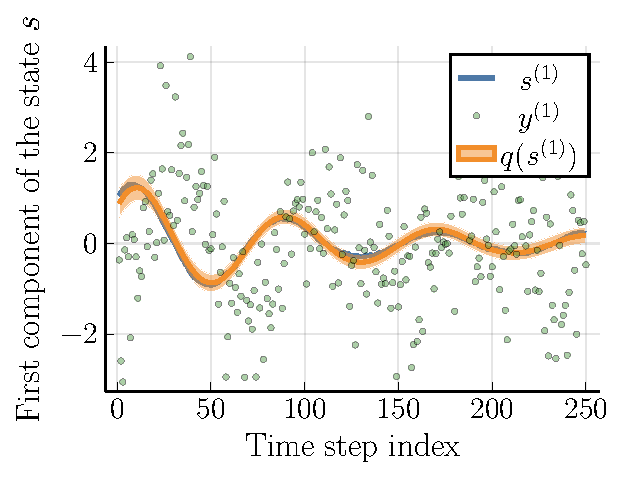
\includegraphics{contents/05-experiments/plots/lds/02-rotating_example_inference_states_1.pdf}
    }
    \caption{Simulated evolution of the first component of the state $s_t$ and its corresponding inferred posterior distribution.}
    \label{fig:sim:rotating_example_inference_states_1}
  \end{subfigure}
  \hfill
  \begin{subfigure}[t]{0.475\textwidth}
    \centering
    \resizebox{\textwidth}{!}{
        % % Recommended preamble:
% \usetikzlibrary{arrows.meta}
% \usetikzlibrary{backgrounds}
% \usepgfplotslibrary{patchplots}
% \usepgfplotslibrary{fillbetween}
% \pgfplotsset{%
%     layers/standard/.define layer set={%
%         background,axis background,axis grid,axis ticks,axis lines,axis tick labels,pre main,main,axis descriptions,axis foreground%
%     }{
%         grid style={/pgfplots/on layer=axis grid},%
%         tick style={/pgfplots/on layer=axis ticks},%
%         axis line style={/pgfplots/on layer=axis lines},%
%         label style={/pgfplots/on layer=axis descriptions},%
%         legend style={/pgfplots/on layer=axis descriptions},%
%         title style={/pgfplots/on layer=axis descriptions},%
%         colorbar style={/pgfplots/on layer=axis descriptions},%
%         ticklabel style={/pgfplots/on layer=axis tick labels},%
%         axis background@ style={/pgfplots/on layer=axis background},%
%         3d box foreground style={/pgfplots/on layer=axis foreground},%
%     },
% }

\begin{tikzpicture}[/tikz/background rectangle/.style={fill={rgb,1:red,1.0;green,1.0;blue,1.0}, fill opacity={1.0}, draw opacity={1.0}}, show background rectangle]
\begin{axis}[point meta max={nan}, point meta min={nan}, legend cell align={left}, legend columns={1}, title={}, title style={at={{(0.5,1)}}, anchor={south}, font={{\fontsize{18 pt}{23.400000000000002 pt}\selectfont}}, color={rgb,1:red,0.0;green,0.0;blue,0.0}, draw opacity={1.0}, rotate={0.0}, align={center}}, legend style={color={rgb,1:red,0.0;green,0.0;blue,0.0}, draw opacity={1.0}, line width={1}, solid, fill={rgb,1:red,1.0;green,1.0;blue,1.0}, fill opacity={1.0}, text opacity={1.0}, font={{\fontsize{14 pt}{18.2 pt}\selectfont}}, text={rgb,1:red,0.0;green,0.0;blue,0.0}, cells={anchor={center}}, at={(0.98, 0.98)}, anchor={north east}}, axis background/.style={fill={rgb,1:red,1.0;green,1.0;blue,1.0}, opacity={1.0}}, anchor={north west}, xshift={1.0mm}, yshift={-1.0mm}, width={99.6mm}, height={74.2mm}, scaled x ticks={false}, xlabel={Time step index}, x tick style={color={rgb,1:red,0.0;green,0.0;blue,0.0}, opacity={1.0}}, x tick label style={color={rgb,1:red,0.0;green,0.0;blue,0.0}, opacity={1.0}, rotate={0}}, xlabel style={at={(ticklabel cs:0.5)}, anchor=near ticklabel, at={{(ticklabel cs:0.5)}}, anchor={near ticklabel}, font={{\fontsize{16 pt}{20.8 pt}\selectfont}}, color={rgb,1:red,0.0;green,0.0;blue,0.0}, draw opacity={1.0}, rotate={0.0}}, xmajorgrids={true}, xmin={-6.469999999999999}, xmax={257.47}, xticklabels={{$0$,$50$,$100$,$150$,$200$,$250$}}, xtick={{0.0,50.0,100.0,150.0,200.0,250.0}}, xtick align={inside}, xticklabel style={font={{\fontsize{14 pt}{18.2 pt}\selectfont}}, color={rgb,1:red,0.0;green,0.0;blue,0.0}, draw opacity={1.0}, rotate={0.0}}, x grid style={color={rgb,1:red,0.0;green,0.0;blue,0.0}, draw opacity={0.1}, line width={0.5}, solid}, axis x line*={left}, x axis line style={color={rgb,1:red,0.0;green,0.0;blue,0.0}, draw opacity={1.0}, line width={1}, solid}, scaled y ticks={false}, ylabel={Second component of the state $s$}, y tick style={color={rgb,1:red,0.0;green,0.0;blue,0.0}, opacity={1.0}}, y tick label style={color={rgb,1:red,0.0;green,0.0;blue,0.0}, opacity={1.0}, rotate={0}}, ylabel style={at={(ticklabel cs:0.5)}, anchor=near ticklabel, at={{(ticklabel cs:0.5)}}, anchor={near ticklabel}, font={{\fontsize{16 pt}{20.8 pt}\selectfont}}, color={rgb,1:red,0.0;green,0.0;blue,0.0}, draw opacity={1.0}, rotate={0.0}}, ymajorgrids={true}, ymin={-3.773440983138788}, ymax={3.9784772025868813}, yticklabels={{$-3$,$-2$,$-1$,$0$,$1$,$2$,$3$}}, ytick={{-3.0,-2.0,-1.0,0.0,1.0,2.0,3.0}}, ytick align={inside}, yticklabel style={font={{\fontsize{14 pt}{18.2 pt}\selectfont}}, color={rgb,1:red,0.0;green,0.0;blue,0.0}, draw opacity={1.0}, rotate={0.0}}, y grid style={color={rgb,1:red,0.0;green,0.0;blue,0.0}, draw opacity={0.1}, line width={0.5}, solid}, axis y line*={left}, y axis line style={color={rgb,1:red,0.0;green,0.0;blue,0.0}, draw opacity={1.0}, line width={1}, solid}, colorbar={false}]
    \addplot[color={rgb,1:red,0.8824;green,0.3412;blue,0.349}, name path={b277fcc4-0eb0-4e6b-aac0-78c6e1dbefbe}, draw opacity={1.0}, line width={2}, solid]
        table[row sep={\\}]
        {
            \\
            1.0  0.9139423264996561  \\
            2.0  0.826681727437719  \\
            3.0  0.7419593801583712  \\
            4.0  0.6395678936444418  \\
            5.0  0.5299299034684026  \\
            6.0  0.40758872952938746  \\
            7.0  0.3235250200132954  \\
            8.0  0.2094682448971536  \\
            9.0  0.10610412391768732  \\
            10.0  -0.003879334667540137  \\
            11.0  -0.11092025905953526  \\
            12.0  -0.20178841757688326  \\
            13.0  -0.29396920543807664  \\
            14.0  -0.36603269742051014  \\
            15.0  -0.44580935330837196  \\
            16.0  -0.5201882194671443  \\
            17.0  -0.5868089638290946  \\
            18.0  -0.6798130575525809  \\
            19.0  -0.733504663017128  \\
            20.0  -0.7850957500182586  \\
            21.0  -0.8343124473037915  \\
            22.0  -0.8929270588444692  \\
            23.0  -0.9305320740802544  \\
            24.0  -0.9828198162406432  \\
            25.0  -1.0007398905275426  \\
            26.0  -1.0189119846286163  \\
            27.0  -1.0402235900460959  \\
            28.0  -1.0610681242100486  \\
            29.0  -1.0718901674619523  \\
            30.0  -1.0728834486335088  \\
            31.0  -1.0608274565877778  \\
            32.0  -1.0380053658637372  \\
            33.0  -1.005066844086312  \\
            34.0  -0.9979462164720146  \\
            35.0  -0.9777157434434284  \\
            36.0  -0.9487928231555944  \\
            37.0  -0.9187367538624566  \\
            38.0  -0.8709764172956501  \\
            39.0  -0.8072523636429166  \\
            40.0  -0.7356988533074598  \\
            41.0  -0.6485395354576281  \\
            42.0  -0.5915739758357391  \\
            43.0  -0.5400651297279758  \\
            44.0  -0.47233229656425957  \\
            45.0  -0.41707688605137694  \\
            46.0  -0.3584722223948842  \\
            47.0  -0.2850328474229366  \\
            48.0  -0.21418437346945865  \\
            49.0  -0.1249360437541312  \\
            50.0  -0.06278737784193722  \\
            51.0  0.003902981478126781  \\
            52.0  0.07939561342095575  \\
            53.0  0.1503231344879653  \\
            54.0  0.23012447476060877  \\
            55.0  0.28829828800698803  \\
            56.0  0.3495409276659987  \\
            57.0  0.40880977308310473  \\
            58.0  0.46057659539662255  \\
            59.0  0.5092355373670427  \\
            60.0  0.5428700897890725  \\
            61.0  0.5674365519512619  \\
            62.0  0.5951309397324664  \\
            63.0  0.622635799882942  \\
            64.0  0.6392722111102564  \\
            65.0  0.6775934796732691  \\
            66.0  0.7154292547034586  \\
            67.0  0.7412716707810474  \\
            68.0  0.7359539727162364  \\
            69.0  0.7381273466544576  \\
            70.0  0.7372970186350419  \\
            71.0  0.7257381783901173  \\
            72.0  0.7085311280239531  \\
            73.0  0.702673216653829  \\
            74.0  0.6815579560109366  \\
            75.0  0.6480522723071585  \\
            76.0  0.6222281020194852  \\
            77.0  0.5722725302089245  \\
            78.0  0.552792643775767  \\
            79.0  0.5134951129820832  \\
            80.0  0.4832046614643037  \\
            81.0  0.44132715145922635  \\
            82.0  0.40428374831331726  \\
            83.0  0.3703882293781391  \\
            84.0  0.32316273265678175  \\
            85.0  0.2826523685892491  \\
            86.0  0.2402038084909223  \\
            87.0  0.20280392745554593  \\
            88.0  0.13366514366150162  \\
            89.0  0.09413923492504898  \\
            90.0  0.07010523888345092  \\
            91.0  0.023187189576477134  \\
            92.0  -0.02145105280624087  \\
            93.0  -0.0541470238737735  \\
            94.0  -0.10242004788955544  \\
            95.0  -0.1140359209843899  \\
            96.0  -0.15116590713876357  \\
            97.0  -0.20123389999566954  \\
            98.0  -0.22288442538409894  \\
            99.0  -0.255758313316565  \\
            100.0  -0.2874200549798491  \\
            101.0  -0.31282121279654884  \\
            102.0  -0.355537579366091  \\
            103.0  -0.37762648664422294  \\
            104.0  -0.3814289173085238  \\
            105.0  -0.4000467648879884  \\
            106.0  -0.4148599534985854  \\
            107.0  -0.40660424013373125  \\
            108.0  -0.39560286044452553  \\
            109.0  -0.37280443203198405  \\
            110.0  -0.35906317064486015  \\
            111.0  -0.3480556694040281  \\
            112.0  -0.34606175675493966  \\
            113.0  -0.334364022157203  \\
            114.0  -0.3399788106828013  \\
            115.0  -0.318717335683333  \\
            116.0  -0.29743382854363126  \\
            117.0  -0.29060101355528095  \\
            118.0  -0.26342922636528876  \\
            119.0  -0.24836700078485785  \\
            120.0  -0.2119509619138454  \\
            121.0  -0.1920370626335401  \\
            122.0  -0.18929406145104422  \\
            123.0  -0.17557760492936383  \\
            124.0  -0.1590870982841247  \\
            125.0  -0.1265323383932624  \\
            126.0  -0.0955418474604389  \\
            127.0  -0.07370291461811844  \\
            128.0  -0.049931285420054386  \\
            129.0  -0.009245735704736132  \\
            130.0  0.01096168157990887  \\
            131.0  0.029290136909315607  \\
            132.0  0.04720586882236372  \\
            133.0  0.06093020967299039  \\
            134.0  0.08995159352810694  \\
            135.0  0.10249029810934993  \\
            136.0  0.1418410626748901  \\
            137.0  0.16430811285311836  \\
            138.0  0.17980366601649675  \\
            139.0  0.20143087139165564  \\
            140.0  0.216320035692829  \\
            141.0  0.20369283376698938  \\
            142.0  0.22794597921020943  \\
            143.0  0.24682348220551437  \\
            144.0  0.2479007338989781  \\
            145.0  0.2554791978042291  \\
            146.0  0.2747549628401238  \\
            147.0  0.28493122912108676  \\
            148.0  0.2840398500974614  \\
            149.0  0.28970038346906596  \\
            150.0  0.2874600193687455  \\
            151.0  0.2931207500692116  \\
            152.0  0.28805204121844513  \\
            153.0  0.26876120310786134  \\
            154.0  0.2543970762844578  \\
            155.0  0.2494208170197601  \\
            156.0  0.2181190249751138  \\
            157.0  0.2093718152694125  \\
            158.0  0.20571187879871172  \\
            159.0  0.20364792804152024  \\
            160.0  0.1863736075379721  \\
            161.0  0.17045637849378148  \\
            162.0  0.135357864822331  \\
            163.0  0.12251301141946089  \\
            164.0  0.11984690091373577  \\
            165.0  0.11401287998732441  \\
            166.0  0.10608274636502717  \\
            167.0  0.08789145526870515  \\
            168.0  0.07563647329121735  \\
            169.0  0.046575057769659825  \\
            170.0  0.03565477390828303  \\
            171.0  0.022851949588578536  \\
            172.0  -0.006711621847547845  \\
            173.0  -0.039111022686803706  \\
            174.0  -0.06016042564357352  \\
            175.0  -0.07884640276391389  \\
            176.0  -0.08884681550932189  \\
            177.0  -0.10350487189859674  \\
            178.0  -0.12633065422182393  \\
            179.0  -0.12563914616369193  \\
            180.0  -0.1432198491433109  \\
            181.0  -0.152971402697168  \\
            182.0  -0.1828578417667424  \\
            183.0  -0.2017916201801862  \\
            184.0  -0.2099466732525659  \\
            185.0  -0.2132710272646842  \\
            186.0  -0.2150271732292239  \\
            187.0  -0.21685644000546564  \\
            188.0  -0.2133107102699198  \\
            189.0  -0.23000489935578422  \\
            190.0  -0.2194748505056568  \\
            191.0  -0.20601570829912125  \\
            192.0  -0.1968392460503198  \\
            193.0  -0.19078248830590191  \\
            194.0  -0.1843855497769603  \\
            195.0  -0.17000030570050195  \\
            196.0  -0.1602922167976657  \\
            197.0  -0.1481081147004638  \\
            198.0  -0.14773064357856014  \\
            199.0  -0.12444957754403206  \\
            200.0  -0.11092464101369667  \\
            201.0  -0.10940526234819432  \\
            202.0  -0.09182205511641474  \\
            203.0  -0.07558432389908695  \\
            204.0  -0.0589516502884399  \\
            205.0  -0.05512455152423886  \\
            206.0  -0.029927278523380077  \\
            207.0  -0.011466900389324913  \\
            208.0  -0.017086654326913954  \\
            209.0  0.01726725326708235  \\
            210.0  0.03007559819449601  \\
            211.0  0.04103302120459719  \\
            212.0  0.05863171162044833  \\
            213.0  0.07066372534764255  \\
            214.0  0.07581430730487937  \\
            215.0  0.08503154175621909  \\
            216.0  0.07744923178761927  \\
            217.0  0.08627124401634062  \\
            218.0  0.10332036808987294  \\
            219.0  0.11040993164627995  \\
            220.0  0.11134366743440904  \\
            221.0  0.126565045103028  \\
            222.0  0.1522966937080266  \\
            223.0  0.1763887062076108  \\
            224.0  0.1937551519470064  \\
            225.0  0.19694801781599228  \\
            226.0  0.2127114265596669  \\
            227.0  0.22456037642771426  \\
            228.0  0.2308189415105174  \\
            229.0  0.24213662069648365  \\
            230.0  0.2408777828578093  \\
            231.0  0.2467884527170218  \\
            232.0  0.24929384951908454  \\
            233.0  0.25643884252022575  \\
            234.0  0.26499906618633423  \\
            235.0  0.263296603102505  \\
            236.0  0.23629103627802042  \\
            237.0  0.23971378709176214  \\
            238.0  0.23875079702685534  \\
            239.0  0.21799400063412455  \\
            240.0  0.22077211141311304  \\
            241.0  0.19597854627090522  \\
            242.0  0.17747164368310644  \\
            243.0  0.16112157125305193  \\
            244.0  0.14491247326445622  \\
            245.0  0.1409243394273801  \\
            246.0  0.13275765736740128  \\
            247.0  0.11598941184605666  \\
            248.0  0.0731015504445369  \\
            249.0  0.051352944405853716  \\
            250.0  0.027377421244445484  \\
        }
        ;
    \addlegendentry {$s^{(2)}$}
    \addplot[color={rgb,1:red,0.6902;green,0.4784;blue,0.6314}, name path={2a8b94b3-4860-4012-a612-94093116599d}, only marks, draw opacity={0.5}, line width={0}, solid, mark={*}, mark size={1.5 pt}, mark repeat={1}, mark options={color={rgb,1:red,0.0;green,0.0;blue,0.0}, draw opacity={0.5}, fill={rgb,1:red,0.6902;green,0.4784;blue,0.6314}, fill opacity={0.5}, line width={0.0}, rotate={0}, solid}]
        table[row sep={\\}]
        {
            \\
            1.0  2.6865034686904483  \\
            2.0  0.6610691815510777  \\
            3.0  2.3382434300604693  \\
            4.0  1.1863787582348655  \\
            5.0  0.7852739961894045  \\
            6.0  1.1165521934460583  \\
            7.0  0.6862219051102325  \\
            8.0  2.326206480620788  \\
            9.0  2.2774087281233646  \\
            10.0  3.759083291670117  \\
            11.0  0.24574643990836487  \\
            12.0  2.2390813868704207  \\
            13.0  1.7221941260314935  \\
            14.0  0.8783167116678238  \\
            15.0  1.4667798973723536  \\
            16.0  2.648559309391919  \\
            17.0  0.9162440389576378  \\
            18.0  1.286166430523954  \\
            19.0  2.481830944904276  \\
            20.0  0.26348404562393557  \\
            21.0  -0.49767581056023924  \\
            22.0  2.45841339706448  \\
            23.0  0.167830894573039  \\
            24.0  1.132639972935233  \\
            25.0  1.2598479286666127  \\
            26.0  0.6150026237167926  \\
            27.0  0.8580243460468271  \\
            28.0  -0.379441544541887  \\
            29.0  -1.1059305819906657  \\
            30.0  -0.7047780119408305  \\
            31.0  0.04072004145372124  \\
            32.0  0.5663572853759095  \\
            33.0  -1.271321080903285  \\
            34.0  -0.13406096165676754  \\
            35.0  0.27115200306861115  \\
            36.0  0.9608336288142406  \\
            37.0  -0.9185651959541206  \\
            38.0  -1.1519345745843226  \\
            39.0  -0.10084946262642958  \\
            40.0  -1.5198038857670202  \\
            41.0  -0.6553133307669605  \\
            42.0  -0.5859890702615758  \\
            43.0  -1.627087021090957  \\
            44.0  -1.4300669685060625  \\
            45.0  -0.17207990850707178  \\
            46.0  -0.7474842492339131  \\
            47.0  -2.380013250464666  \\
            48.0  -2.019032743724468  \\
            49.0  -2.4398153008351473  \\
            50.0  -0.6607066250222813  \\
            51.0  -2.376899124467764  \\
            52.0  -0.6851711207647544  \\
            53.0  -1.3480739281273344  \\
            54.0  -3.5540470722220237  \\
            55.0  -1.2983849588817857  \\
            56.0  -1.5244969131752595  \\
            57.0  -1.6735364636313514  \\
            58.0  -0.4835916978370802  \\
            59.0  -0.7031319954976907  \\
            60.0  -1.127304256396235  \\
            61.0  -1.2299229987585039  \\
            62.0  -1.0071616108756438  \\
            63.0  -1.2566003655814422  \\
            64.0  -0.9216579892703302  \\
            65.0  -0.3270484048098377  \\
            66.0  -0.11198876586159223  \\
            67.0  -0.26667387937713594  \\
            68.0  0.18134006187553064  \\
            69.0  0.326410656814323  \\
            70.0  0.4622953106848001  \\
            71.0  0.5328893872618697  \\
            72.0  0.5040861131207726  \\
            73.0  -0.2043928830264427  \\
            74.0  2.070110471425899  \\
            75.0  -1.0092224841422182  \\
            76.0  -0.09057123074773632  \\
            77.0  -0.2630778716623074  \\
            78.0  -0.46100623004134733  \\
            79.0  0.39783626289855023  \\
            80.0  2.2084477137456284  \\
            81.0  0.9906905182009027  \\
            82.0  -0.6137728823636632  \\
            83.0  1.1765946934799019  \\
            84.0  0.9431882273357916  \\
            85.0  -0.2034676501742606  \\
            86.0  0.8352127619283574  \\
            87.0  1.3374310336817794  \\
            88.0  1.8326201287181365  \\
            89.0  0.776640685804237  \\
            90.0  -1.9964739256137567  \\
            91.0  0.7459313455670961  \\
            92.0  -0.6822076206780749  \\
            93.0  -0.7376037792638788  \\
            94.0  0.8685030614269587  \\
            95.0  1.2360165776705268  \\
            96.0  -1.1874603496346179  \\
            97.0  1.9791418428326426  \\
            98.0  -1.0990999052892845  \\
            99.0  2.288573209597804  \\
            100.0  0.6506021112475333  \\
            101.0  1.3478384738069726  \\
            102.0  0.37398959442153695  \\
            103.0  -0.6699727562926593  \\
            104.0  -0.7977661721418449  \\
            105.0  0.657917871176291  \\
            106.0  0.389668128114737  \\
            107.0  0.24732874863436244  \\
            108.0  -1.4385617575829293  \\
            109.0  -0.2500398038255182  \\
            110.0  -0.07050976788558909  \\
            111.0  -0.21243543017334401  \\
            112.0  0.1417870033713586  \\
            113.0  -0.29708639963510586  \\
            114.0  0.41431040013233517  \\
            115.0  1.0615315761039532  \\
            116.0  0.08829362464490259  \\
            117.0  -0.5897428390687512  \\
            118.0  -1.3417129465148463  \\
            119.0  0.5081674123816606  \\
            120.0  -0.9080454760440475  \\
            121.0  -1.275598100717477  \\
            122.0  0.1919700514146484  \\
            123.0  -0.3732507412806464  \\
            124.0  -0.9181148134921402  \\
            125.0  -1.971573968908915  \\
            126.0  -0.5859254708840578  \\
            127.0  -0.6083964616231179  \\
            128.0  -1.072251663995012  \\
            129.0  -0.533917285526837  \\
            130.0  -0.10109156809324232  \\
            131.0  -0.889979952330008  \\
            132.0  -0.4589738962612315  \\
            133.0  -1.0463974329142296  \\
            134.0  -0.2125587378740768  \\
            135.0  -0.32098070549165636  \\
            136.0  0.25648396154227865  \\
            137.0  -1.2602171148134897  \\
            138.0  -1.3032216825921188  \\
            139.0  0.9621258771576597  \\
            140.0  -0.05066239867796257  \\
            141.0  0.030357168140001334  \\
            142.0  -0.409327474389966  \\
            143.0  -0.6184164905073706  \\
            144.0  -0.5623873446307848  \\
            145.0  -0.24092474139530617  \\
            146.0  1.0964630720225874  \\
            147.0  -0.7592186482097448  \\
            148.0  0.019561846218655227  \\
            149.0  -0.490510707908382  \\
            150.0  -1.72073899283562  \\
            151.0  0.4626674473075348  \\
            152.0  1.250924098010326  \\
            153.0  0.292769534174838  \\
            154.0  1.3909763579734946  \\
            155.0  -0.7273402316053436  \\
            156.0  -0.19014209211303892  \\
            157.0  -0.7400383371444402  \\
            158.0  -1.303394356172639  \\
            159.0  0.5014829789274512  \\
            160.0  0.18936153868567357  \\
            161.0  1.9689317447080905  \\
            162.0  -0.360530811400277  \\
            163.0  0.5036913740071914  \\
            164.0  -0.9535120939361754  \\
            165.0  -0.3208582214780097  \\
            166.0  2.4951593097229114  \\
            167.0  -0.5573712641245929  \\
            168.0  0.18847773548097235  \\
            169.0  1.8904728121295091  \\
            170.0  0.8961719879848076  \\
            171.0  -0.8276797089842443  \\
            172.0  1.2955435084017697  \\
            173.0  2.0197294560950194  \\
            174.0  -1.0664386421574785  \\
            175.0  0.6882393379542178  \\
            176.0  1.3233511874024162  \\
            177.0  2.093041228325718  \\
            178.0  -0.4134601183381302  \\
            179.0  1.5970697459736662  \\
            180.0  -1.3323770912809598  \\
            181.0  0.17557655410197526  \\
            182.0  2.051491310589964  \\
            183.0  -0.30018925076670744  \\
            184.0  1.4526956634985957  \\
            185.0  0.9146937684721315  \\
            186.0  0.03128593837357618  \\
            187.0  -0.13370535398757633  \\
            188.0  -1.1463800726627018  \\
            189.0  -1.2048652533209838  \\
            190.0  -1.015322207182953  \\
            191.0  -1.965722426801884  \\
            192.0  -1.1870466234504553  \\
            193.0  -0.4277646908539018  \\
            194.0  1.4052730581478545  \\
            195.0  0.009819201582386083  \\
            196.0  0.7839231291988403  \\
            197.0  -0.5914144140350177  \\
            198.0  1.5581572737883265  \\
            199.0  -0.2703232553011827  \\
            200.0  1.0770073738499093  \\
            201.0  0.5578735247288018  \\
            202.0  1.7807338428457837  \\
            203.0  2.037303951755668  \\
            204.0  -0.10936628936701313  \\
            205.0  -0.5456617375842041  \\
            206.0  -0.6886804483528325  \\
            207.0  -1.2571089843064878  \\
            208.0  -1.7215132690380863  \\
            209.0  0.08670140245278918  \\
            210.0  1.4444057998172384  \\
            211.0  1.0839005414250358  \\
            212.0  1.6707723049709937  \\
            213.0  -0.42697982959121916  \\
            214.0  -0.8986926171606712  \\
            215.0  0.7114299173358284  \\
            216.0  -1.214903761140543  \\
            217.0  -0.3551670645839455  \\
            218.0  -0.3425300449019031  \\
            219.0  1.9202065542984064  \\
            220.0  0.6317084761353249  \\
            221.0  -0.1851581506027628  \\
            222.0  0.8989311368910309  \\
            223.0  0.6554435951061048  \\
            224.0  0.49611402419480444  \\
            225.0  -1.3210707539195674  \\
            226.0  -0.7894098496276933  \\
            227.0  0.2840307972466564  \\
            228.0  0.7921099724793761  \\
            229.0  0.40049018859011326  \\
            230.0  0.6105042634695863  \\
            231.0  0.6188408843293506  \\
            232.0  -1.6029946287382706  \\
            233.0  -0.22616457883764707  \\
            234.0  0.7783643434606038  \\
            235.0  -0.7514975110596412  \\
            236.0  -0.5571857201195602  \\
            237.0  -0.5000718302584817  \\
            238.0  -1.0096728835221818  \\
            239.0  -0.5246807205812757  \\
            240.0  1.0392028208632964  \\
            241.0  -1.1964766315924071  \\
            242.0  1.1493149380044865  \\
            243.0  0.8520240640682426  \\
            244.0  2.0076560686852365  \\
            245.0  1.516683889749124  \\
            246.0  0.15629583096320263  \\
            247.0  1.7113785911244586  \\
            248.0  0.2635291735834718  \\
            249.0  0.7053764204846618  \\
            250.0  -0.4418834718210959  \\
        }
        ;
    \addlegendentry {$y^{(2)}$}
    \addplot+[line width={0}, draw opacity={0}, fill={rgb,1:red,0.4627;green,0.7176;blue,0.698}, fill opacity={0.5}, mark={none}, forget plot]
        coordinates {
            (1,1.019277409595826)
            (2,0.937920976332208)
            (3,0.8520507312894767)
            (4,0.7621681172781777)
            (5,0.669439115923124)
            (6,0.5745092877672441)
            (7,0.4778885540378565)
            (8,0.37981952625806953)
            (9,0.2813320289302292)
            (10,0.18300613565918686)
            (11,0.08536997946350212)
            (12,-0.011186744172810924)
            (13,-0.10601544839981059)
            (14,-0.19861033166842443)
            (15,-0.28818677930719433)
            (16,-0.374254642169673)
            (17,-0.45655103691375626)
            (18,-0.534593670576785)
            (19,-0.6077920152190482)
            (20,-0.6757648692241828)
            (21,-0.7385571753541718)
            (22,-0.7958615918642674)
            (23,-0.8472349671070474)
            (24,-0.8919347895402221)
            (25,-0.930250539589614)
            (26,-0.9623642121390357)
            (27,-0.987543999476449)
            (28,-1.006290457497983)
            (29,-1.0186317572317818)
            (30,-1.0244408748394023)
            (31,-1.0240556271632535)
            (32,-1.0170549114739609)
            (33,-1.0041028368040372)
            (34,-0.9851868831282168)
            (35,-0.9604095570507863)
            (36,-0.9299526902056722)
            (37,-0.8943518005843163)
            (38,-0.8537917545811153)
            (39,-0.8084607313280332)
            (40,-0.758329704658416)
            (41,-0.7045063057911225)
            (42,-0.6472755542943628)
            (43,-0.5869382959188648)
            (44,-0.5239575056569665)
            (45,-0.4587301055296177)
            (46,-0.3915782138369626)
            (47,-0.3229720208726418)
            (48,-0.2535955376003567)
            (49,-0.18364951628793177)
            (50,-0.11384505950187791)
            (51,-0.04459403084928743)
            (52,0.023757464240332562)
            (53,0.09114137176299784)
            (54,0.1569437679989614)
            (55,0.22039375999138539)
            (56,0.2812577552964301)
            (57,0.33931735068673263)
            (58,0.3944564021592386)
            (59,0.4456551611180235)
            (60,0.4928469324536207)
            (61,0.5360452041938829)
            (62,0.5749748724336367)
            (63,0.6096668745367365)
            (64,0.6398595237142635)
            (65,0.665340703637575)
            (66,0.6862040768495217)
            (67,0.7023212221776932)
            (68,0.7138740463167764)
            (69,0.7203542588585959)
            (70,0.72214596540079)
            (71,0.7192499185868778)
            (72,0.711850168592923)
            (73,0.6999841136233752)
            (74,0.6839707625109175)
            (75,0.6636376722797634)
            (76,0.6396764416711794)
            (77,0.612095614157788)
            (78,0.5813893123802784)
            (79,0.5473028972319902)
            (80,0.5104172153018951)
            (81,0.4709573102403396)
            (82,0.4291683444557128)
            (83,0.38528026047583946)
            (84,0.33969278646308554)
            (85,0.2930270907172081)
            (86,0.24551660570468337)
            (87,0.19729426089475693)
            (88,0.1490013511691946)
            (89,0.10054753692949756)
            (90,0.05242968868271645)
            (91,0.005104859281574017)
            (92,-0.04103220490913474)
            (93,-0.08589008418774752)
            (94,-0.12940165452550095)
            (95,-0.17116441190843054)
            (96,-0.21092010045693885)
            (97,-0.2484682041087624)
            (98,-0.2836626367390919)
            (99,-0.3162403595643061)
            (100,-0.34613002238043955)
            (101,-0.37333771652820197)
            (102,-0.3979588088452192)
            (103,-0.41957971033232866)
            (104,-0.4383080231639134)
            (105,-0.4537082648068601)
            (106,-0.4660909412432485)
            (107,-0.4753540146963264)
            (108,-0.48145159241225294)
            (109,-0.48462795666316105)
            (110,-0.48481050883719035)
            (111,-0.48220876767408793)
            (112,-0.47645513802984857)
            (113,-0.4679709313772932)
            (114,-0.45659535219219965)
            (115,-0.44255482739412455)
            (116,-0.4263496962946225)
            (117,-0.4078625774674309)
            (118,-0.38713038012507583)
            (119,-0.3646553342492902)
            (120,-0.3400716577375063)
            (121,-0.31395497804856554)
            (122,-0.28632853145610654)
            (123,-0.25727617028085026)
            (124,-0.2270160803832706)
            (125,-0.19618988737501034)
            (126,-0.1648318348519643)
            (127,-0.1331224372444316)
            (128,-0.10160069588107513)
            (129,-0.06968376694830661)
            (130,-0.03790125012832334)
            (131,-0.0065686789115227675)
            (132,0.02463180576209078)
            (133,0.055199030593025146)
            (134,0.08479024482831499)
            (135,0.11400812828694587)
            (136,0.14218240206221536)
            (137,0.16946520942985724)
            (138,0.19541668173399654)
            (139,0.21978995869600804)
            (140,0.2423438070390423)
            (141,0.2633257963018733)
            (142,0.2823988549550714)
            (143,0.2995111805930665)
            (144,0.31456771551625295)
            (145,0.3278157391746392)
            (146,0.33909500758474853)
            (147,0.3480769519655252)
            (148,0.35485253737460976)
            (149,0.35945542016660237)
            (150,0.36143931592119705)
            (151,0.3610969085422634)
            (152,0.35854418841236024)
            (153,0.3539435332259799)
            (154,0.34751398380655396)
            (155,0.33910997267205445)
            (156,0.3289103088726772)
            (157,0.31698067159895543)
            (158,0.3029266574067059)
            (159,0.28692256859011184)
            (160,0.2694826826883632)
            (161,0.25033171956185674)
            (162,0.2297105697377662)
            (163,0.2082031368605485)
            (164,0.18546510092179974)
            (165,0.16215029963453195)
            (166,0.13836881670551612)
            (167,0.11407262634910188)
            (168,0.0894020280956559)
            (169,0.06455132190912909)
            (170,0.03952847509790377)
            (171,0.014649993313948968)
            (172,-0.009888628894965676)
            (173,-0.03392204935534704)
            (174,-0.057357005369115185)
            (175,-0.08004201787634739)
            (176,-0.10187813241520577)
            (177,-0.12273585076091663)
            (178,-0.14252123869344685)
            (179,-0.1609700368007038)
            (180,-0.17781288194175165)
            (181,-0.1935559487982603)
            (182,-0.2075274198981314)
            (183,-0.21970613932648694)
            (184,-0.23012816416501977)
            (185,-0.23882671110708964)
            (186,-0.24569538215721215)
            (187,-0.25051507086622465)
            (188,-0.2533809769167398)
            (189,-0.25464897078108034)
            (190,-0.2543634868859117)
            (191,-0.2524382685959071)
            (192,-0.24930672287558156)
            (193,-0.2449968029772134)
            (194,-0.23954815089586143)
            (195,-0.23309104797005786)
            (196,-0.22536105291709996)
            (197,-0.21632600130765106)
            (198,-0.20630705643875769)
            (199,-0.19539897469331155)
            (200,-0.18379857790845516)
            (201,-0.17153663152587528)
            (202,-0.15835795556353574)
            (203,-0.14448903256155796)
            (204,-0.12941520029882686)
            (205,-0.11401607095942973)
            (206,-0.09795718975475415)
            (207,-0.08164298291125743)
            (208,-0.06541541326734181)
            (209,-0.0495193494618031)
            (210,-0.033677654811894775)
            (211,-0.01794240082444349)
            (212,-0.0022570028006499696)
            (213,0.013243375856030562)
            (214,0.028465074688689748)
            (215,0.04355308761608354)
            (216,0.05843945305515122)
            (217,0.07289311105617938)
            (218,0.08724119927569222)
            (219,0.10095604134212513)
            (220,0.11379454838575088)
            (221,0.12595996347599106)
            (222,0.13745471843096094)
            (223,0.14827653274109348)
            (224,0.15805137797239086)
            (225,0.16691131650639188)
            (226,0.17462999131652676)
            (227,0.18122534117365338)
            (228,0.18706547126683556)
            (229,0.19148594628421078)
            (230,0.19495736271052289)
            (231,0.19688773982964214)
            (232,0.19784084968153975)
            (233,0.19746147443691733)
            (234,0.19567592600898553)
            (235,0.19234278963663828)
            (236,0.18825900279838492)
            (237,0.18314820450907768)
            (238,0.17669774532072766)
            (239,0.16897249501844083)
            (240,0.16005021927436694)
            (241,0.14978529541142213)
            (242,0.13851258129032062)
            (243,0.126720394642869)
            (244,0.11444094643255319)
            (245,0.10152871557314683)
            (246,0.08782958764924459)
            (247,0.07392841054508009)
            (248,0.05991823127055344)
            (249,0.0457709550517576)
            (250,0.03171424689279253)
            (250,-0.1472542500369393)
            (249,-0.13208458411453958)
            (248,-0.1168764987420381)
            (247,-0.10186174165682069)
            (246,-0.08701519637736252)
            (245,-0.07243178913470105)
            (244,-0.0586971785985962)
            (243,-0.04565704405650822)
            (242,-0.03316470913767122)
            (241,-0.021250362026363184)
            (240,-0.010399522325696464)
            (239,-0.0009435749784872105)
            (238,0.00726714328368297)
            (237,0.01415936301057033)
            (236,0.0196730508413569)
            (235,0.024125915619591237)
            (234,0.027799483383695034)
            (233,0.029901971887002055)
            (232,0.03057982978301721)
            (231,0.029911552458043167)
            (230,0.02825684186219915)
            (229,0.025056001368249425)
            (228,0.02090460615914283)
            (227,0.015335116256144005)
            (226,0.009014445207532834)
            (225,0.0015763651010943514)
            (224,-0.0069957913315441544)
            (223,-0.016474988714310218)
            (222,-0.026993175296461974)
            (221,-0.03817672922022858)
            (220,-0.05002424143322569)
            (219,-0.06253941457278417)
            (218,-0.07592708952259876)
            (217,-0.0899460259057982)
            (216,-0.10407056906030296)
            (215,-0.11862997554311533)
            (214,-0.133395329168228)
            (213,-0.14830077022612437)
            (212,-0.16349329289955983)
            (211,-0.17888108374133074)
            (210,-0.19433063017699997)
            (209,-0.2098999376322812)
            (208,-0.22553810028896853)
            (207,-0.24152314925853863)
            (206,-0.2576108310975944)
            (205,-0.27345951859309753)
            (204,-0.2886648481616342)
            (203,-0.30356107698757484)
            (202,-0.31726815310378864)
            (201,-0.3303000793413835)
            (200,-0.3424295204064673)
            (199,-0.3539106392538388)
            (198,-0.36471152026851617)
            (197,-0.3746340906678395)
            (196,-0.38358227520486166)
            (195,-0.3912335563965919)
            (194,-0.39761874080395176)
            (193,-0.40300093818607374)
            (192,-0.40724858984148027)
            (191,-0.4103208556441762)
            (190,-0.41218868531505315)
            (189,-0.41241769427354097)
            (188,-0.41109329542272427)
            (187,-0.4081703549633685)
            (186,-0.40329245383351087)
            (185,-0.39636399696689856)
            (184,-0.38760384721391866)
            (183,-0.37711830574215754)
            (182,-0.36487419752939393)
            (181,-0.35083563453842675)
            (180,-0.33502405557877757)
            (179,-0.31811165943743464)
            (178,-0.29959273433859146)
            (177,-0.27973717019804795)
            (176,-0.25880979894747824)
            (175,-0.23690515500532489)
            (174,-0.2141533468863544)
            (173,-0.19065393269724443)
            (172,-0.1665589729297773)
            (171,-0.14196227536454586)
            (170,-0.11702967841000275)
            (169,-0.0919571132941172)
            (168,-0.0670614539805954)
            (167,-0.04235096085766353)
            (166,-0.018020146840314527)
            (165,0.005790558668058804)
            (164,0.02912913570820419)
            (163,0.05188553818100386)
            (162,0.0734060468263445)
            (161,0.0940351768225299)
            (160,0.1131892907876284)
            (159,0.13062782856576885)
            (158,0.1466264565803585)
            (157,0.16067133023633223)
            (156,0.17258861670137274)
            (155,0.18277321454054596)
            (154,0.19115995395118884)
            (153,0.19757053780379805)
            (152,0.20215103615659683)
            (151,0.20468288960324052)
            (150,0.2050041691666108)
            (149,0.20299928942988005)
            (148,0.1983759173553573)
            (147,0.19158062469876222)
            (146,0.18257997060173278)
            (145,0.17128312667322595)
            (144,0.15801871403821027)
            (143,0.14294694086472798)
            (142,0.1258204016813671)
            (141,0.10673393780762619)
            (140,0.08573904672143559)
            (139,0.06317241028496356)
            (138,0.03878599035033514)
            (137,0.012820480382949306)
            (136,-0.014477860761238887)
            (135,-0.04266981614907975)
            (134,-0.07190821821974297)
            (133,-0.10152350047316272)
            (132,-0.13211906308789423)
            (131,-0.16335286751798592)
            (130,-0.1947244279037283)
            (129,-0.22655224918450567)
            (128,-0.25852138556865945)
            (127,-0.29010275081277226)
            (126,-0.32187961275140436)
            (125,-0.3533132908112511)
            (124,-0.3842234759058464)
            (123,-0.4145760043172395)
            (122,-0.4437291972640999)
            (121,-0.47146467792437724)
            (120,-0.49769826365665787)
            (119,-0.5224062504206953)
            (118,-0.5450124111934185)
            (117,-0.565881806290587)
            (116,-0.5845113753358996)
            (115,-0.6008632877870911)
            (114,-0.6150539344425402)
            (113,-0.6265819414463853)
            (112,-0.6352198321861563)
            (111,-0.6411273689926835)
            (110,-0.6438822575721435)
            (109,-0.6438511959167206)
            (108,-0.6408238895915317)
            (107,-0.6348723182043778)
            (106,-0.6257517707277089)
            (105,-0.6135079321245481)
            (104,-0.5982428800592308)
            (103,-0.5796464177202973)
            (102,-0.558154621586743)
            (101,-0.533660776733353)
            (100,-0.5065796536168321)
            (99,-0.4768173539143147)
            (98,-0.4443695264624416)
            (97,-0.40930950973337443)
            (96,-0.3719025474349914)
            (95,-0.33229710851824523)
            (94,-0.29069622444492516)
            (93,-0.2473607480761832)
            (92,-0.20269580637530182)
            (91,-0.1567711131823446)
            (90,-0.10968058346555587)
            (89,-0.061821301829298014)
            (88,-0.013652440026435536)
            (87,0.03432729275595281)
            (86,0.08220673582072496)
            (85,0.12934348650026517)
            (84,0.17560394875551477)
            (83,0.22075450659446347)
            (82,0.26417432463314783)
            (81,0.30546454738016804)
            (80,0.3443966562272371)
            (79,0.3807274618227927)
            (78,0.414234425231901)
            (77,0.44433970175463056)
            (76,0.47130137669106414)
            (75,0.49462914569515926)
            (74,0.5143185638209726)
            (73,0.5296823000313949)
            (72,0.5408971054175084)
            (71,0.5476481758002532)
            (70,0.5499020589940452)
            (69,0.5474782307135242)
            (68,0.5403788822743201)
            (67,0.5282221147660523)
            (66,0.5115175462869925)
            (65,0.4900835977830359)
            (64,0.46404792408366413)
            (63,0.43331494083068545)
            (62,0.39809366179693145)
            (61,0.358641503351096)
            (60,0.3149221408065463)
            (59,0.2672042609127626)
            (58,0.21546704817759116)
            (57,0.15976910698225905)
            (56,0.1011215007702583)
            (55,0.03963127861000043)
            (54,-0.024492466310608224)
            (53,-0.09102546711034819)
            (52,-0.15920597164084563)
            (51,-0.22842881440648702)
            (50,-0.29863412374156895)
            (49,-0.36948321305858534)
            (48,-0.44057069268093507)
            (47,-0.5111908140414629)
            (46,-0.5811468906350514)
            (45,-0.6497575283302744)
            (44,-0.7165535536003804)
            (43,-0.7812121267125427)
            (42,-0.8433337461948798)
            (41,-0.9024509055270451)
            (40,-0.9582562166971166)
            (39,-1.0104560955338648)
            (38,-1.057932372416046)
            (37,-1.1007016836066517)
            (36,-1.1385618173218595)
            (35,-1.171312536947018)
            (34,-1.1984020234399537)
            (33,-1.2196317197107291)
            (32,-1.234882564675762)
            (31,-1.2441513584832642)
            (30,-1.2467598080385776)
            (29,-1.243117067542799)
            (28,-1.2328762609607498)
            (27,-1.2161588047977274)
            (26,-1.1929348026532458)
            (25,-1.1627061210250564)
            (24,-1.1262112207357835)
            (23,-1.0832788878217037)
            (22,-1.033634274385619)
            (21,-0.9780379525488754)
            (20,-0.9169540270597951)
            (19,-0.8507130777561355)
            (18,-0.7792950450532256)
            (17,-0.7031070216015439)
            (16,-0.6227658271840752)
            (15,-0.538779888919287)
            (14,-0.4514375656892555)
            (13,-0.36125338071433516)
            (12,-0.2690348300677702)
            (11,-0.17530875302458238)
            (10,-0.08074260527118918)
            (9,0.014257532599217082)
            (8,0.10914994523711596)
            (7,0.20334411482151477)
            (6,0.2958032703236102)
            (5,0.3862817374556495)
            (4,0.47427082355098105)
            (3,0.5591309032060677)
            (2,0.6397070355094135)
            (1,0.7155142716751246)
            (1,1.019277409595826)
        }
        ;
    \addplot+[line width={0}, draw opacity={0}, fill={rgb,1:red,0.4627;green,0.7176;blue,0.698}, fill opacity={0.5}, mark={none}, forget plot]
        coordinates {
            (1,1.019277409595826)
            (2,0.937920976332208)
            (3,0.8520507312894767)
            (4,0.7621681172781777)
            (5,0.669439115923124)
            (6,0.5745092877672441)
            (7,0.4778885540378565)
            (8,0.37981952625806953)
            (9,0.2813320289302292)
            (10,0.18300613565918686)
            (11,0.08536997946350212)
            (12,-0.011186744172810924)
            (13,-0.10601544839981059)
            (14,-0.19861033166842443)
            (15,-0.28818677930719433)
            (16,-0.374254642169673)
            (17,-0.45655103691375626)
            (18,-0.534593670576785)
            (19,-0.6077920152190482)
            (20,-0.6757648692241828)
            (21,-0.7385571753541718)
            (22,-0.7958615918642674)
            (23,-0.8472349671070474)
            (24,-0.8919347895402221)
            (25,-0.930250539589614)
            (26,-0.9623642121390357)
            (27,-0.987543999476449)
            (28,-1.006290457497983)
            (29,-1.0186317572317818)
            (30,-1.0244408748394023)
            (31,-1.0240556271632535)
            (32,-1.0170549114739609)
            (33,-1.0041028368040372)
            (34,-0.9851868831282168)
            (35,-0.9604095570507863)
            (36,-0.9299526902056722)
            (37,-0.8943518005843163)
            (38,-0.8537917545811153)
            (39,-0.8084607313280332)
            (40,-0.758329704658416)
            (41,-0.7045063057911225)
            (42,-0.6472755542943628)
            (43,-0.5869382959188648)
            (44,-0.5239575056569665)
            (45,-0.4587301055296177)
            (46,-0.3915782138369626)
            (47,-0.3229720208726418)
            (48,-0.2535955376003567)
            (49,-0.18364951628793177)
            (50,-0.11384505950187791)
            (51,-0.04459403084928743)
            (52,0.023757464240332562)
            (53,0.09114137176299784)
            (54,0.1569437679989614)
            (55,0.22039375999138539)
            (56,0.2812577552964301)
            (57,0.33931735068673263)
            (58,0.3944564021592386)
            (59,0.4456551611180235)
            (60,0.4928469324536207)
            (61,0.5360452041938829)
            (62,0.5749748724336367)
            (63,0.6096668745367365)
            (64,0.6398595237142635)
            (65,0.665340703637575)
            (66,0.6862040768495217)
            (67,0.7023212221776932)
            (68,0.7138740463167764)
            (69,0.7203542588585959)
            (70,0.72214596540079)
            (71,0.7192499185868778)
            (72,0.711850168592923)
            (73,0.6999841136233752)
            (74,0.6839707625109175)
            (75,0.6636376722797634)
            (76,0.6396764416711794)
            (77,0.612095614157788)
            (78,0.5813893123802784)
            (79,0.5473028972319902)
            (80,0.5104172153018951)
            (81,0.4709573102403396)
            (82,0.4291683444557128)
            (83,0.38528026047583946)
            (84,0.33969278646308554)
            (85,0.2930270907172081)
            (86,0.24551660570468337)
            (87,0.19729426089475693)
            (88,0.1490013511691946)
            (89,0.10054753692949756)
            (90,0.05242968868271645)
            (91,0.005104859281574017)
            (92,-0.04103220490913474)
            (93,-0.08589008418774752)
            (94,-0.12940165452550095)
            (95,-0.17116441190843054)
            (96,-0.21092010045693885)
            (97,-0.2484682041087624)
            (98,-0.2836626367390919)
            (99,-0.3162403595643061)
            (100,-0.34613002238043955)
            (101,-0.37333771652820197)
            (102,-0.3979588088452192)
            (103,-0.41957971033232866)
            (104,-0.4383080231639134)
            (105,-0.4537082648068601)
            (106,-0.4660909412432485)
            (107,-0.4753540146963264)
            (108,-0.48145159241225294)
            (109,-0.48462795666316105)
            (110,-0.48481050883719035)
            (111,-0.48220876767408793)
            (112,-0.47645513802984857)
            (113,-0.4679709313772932)
            (114,-0.45659535219219965)
            (115,-0.44255482739412455)
            (116,-0.4263496962946225)
            (117,-0.4078625774674309)
            (118,-0.38713038012507583)
            (119,-0.3646553342492902)
            (120,-0.3400716577375063)
            (121,-0.31395497804856554)
            (122,-0.28632853145610654)
            (123,-0.25727617028085026)
            (124,-0.2270160803832706)
            (125,-0.19618988737501034)
            (126,-0.1648318348519643)
            (127,-0.1331224372444316)
            (128,-0.10160069588107513)
            (129,-0.06968376694830661)
            (130,-0.03790125012832334)
            (131,-0.0065686789115227675)
            (132,0.02463180576209078)
            (133,0.055199030593025146)
            (134,0.08479024482831499)
            (135,0.11400812828694587)
            (136,0.14218240206221536)
            (137,0.16946520942985724)
            (138,0.19541668173399654)
            (139,0.21978995869600804)
            (140,0.2423438070390423)
            (141,0.2633257963018733)
            (142,0.2823988549550714)
            (143,0.2995111805930665)
            (144,0.31456771551625295)
            (145,0.3278157391746392)
            (146,0.33909500758474853)
            (147,0.3480769519655252)
            (148,0.35485253737460976)
            (149,0.35945542016660237)
            (150,0.36143931592119705)
            (151,0.3610969085422634)
            (152,0.35854418841236024)
            (153,0.3539435332259799)
            (154,0.34751398380655396)
            (155,0.33910997267205445)
            (156,0.3289103088726772)
            (157,0.31698067159895543)
            (158,0.3029266574067059)
            (159,0.28692256859011184)
            (160,0.2694826826883632)
            (161,0.25033171956185674)
            (162,0.2297105697377662)
            (163,0.2082031368605485)
            (164,0.18546510092179974)
            (165,0.16215029963453195)
            (166,0.13836881670551612)
            (167,0.11407262634910188)
            (168,0.0894020280956559)
            (169,0.06455132190912909)
            (170,0.03952847509790377)
            (171,0.014649993313948968)
            (172,-0.009888628894965676)
            (173,-0.03392204935534704)
            (174,-0.057357005369115185)
            (175,-0.08004201787634739)
            (176,-0.10187813241520577)
            (177,-0.12273585076091663)
            (178,-0.14252123869344685)
            (179,-0.1609700368007038)
            (180,-0.17781288194175165)
            (181,-0.1935559487982603)
            (182,-0.2075274198981314)
            (183,-0.21970613932648694)
            (184,-0.23012816416501977)
            (185,-0.23882671110708964)
            (186,-0.24569538215721215)
            (187,-0.25051507086622465)
            (188,-0.2533809769167398)
            (189,-0.25464897078108034)
            (190,-0.2543634868859117)
            (191,-0.2524382685959071)
            (192,-0.24930672287558156)
            (193,-0.2449968029772134)
            (194,-0.23954815089586143)
            (195,-0.23309104797005786)
            (196,-0.22536105291709996)
            (197,-0.21632600130765106)
            (198,-0.20630705643875769)
            (199,-0.19539897469331155)
            (200,-0.18379857790845516)
            (201,-0.17153663152587528)
            (202,-0.15835795556353574)
            (203,-0.14448903256155796)
            (204,-0.12941520029882686)
            (205,-0.11401607095942973)
            (206,-0.09795718975475415)
            (207,-0.08164298291125743)
            (208,-0.06541541326734181)
            (209,-0.0495193494618031)
            (210,-0.033677654811894775)
            (211,-0.01794240082444349)
            (212,-0.0022570028006499696)
            (213,0.013243375856030562)
            (214,0.028465074688689748)
            (215,0.04355308761608354)
            (216,0.05843945305515122)
            (217,0.07289311105617938)
            (218,0.08724119927569222)
            (219,0.10095604134212513)
            (220,0.11379454838575088)
            (221,0.12595996347599106)
            (222,0.13745471843096094)
            (223,0.14827653274109348)
            (224,0.15805137797239086)
            (225,0.16691131650639188)
            (226,0.17462999131652676)
            (227,0.18122534117365338)
            (228,0.18706547126683556)
            (229,0.19148594628421078)
            (230,0.19495736271052289)
            (231,0.19688773982964214)
            (232,0.19784084968153975)
            (233,0.19746147443691733)
            (234,0.19567592600898553)
            (235,0.19234278963663828)
            (236,0.18825900279838492)
            (237,0.18314820450907768)
            (238,0.17669774532072766)
            (239,0.16897249501844083)
            (240,0.16005021927436694)
            (241,0.14978529541142213)
            (242,0.13851258129032062)
            (243,0.126720394642869)
            (244,0.11444094643255319)
            (245,0.10152871557314683)
            (246,0.08782958764924459)
            (247,0.07392841054508009)
            (248,0.05991823127055344)
            (249,0.0457709550517576)
            (250,0.03171424689279253)
            (250,0.21068274382252436)
            (249,0.22362649421805478)
            (248,0.236712961283145)
            (247,0.24971856274698087)
            (246,0.2626743716758517)
            (245,0.2754892202809947)
            (244,0.2875790714637026)
            (243,0.2990978333422462)
            (242,0.31018987171831247)
            (241,0.3208209528492074)
            (240,0.33049996087443034)
            (239,0.3388885650153689)
            (238,0.3461283473577723)
            (237,0.352137046007585)
            (236,0.35684495475541295)
            (235,0.3605596636536853)
            (234,0.36355236863427604)
            (233,0.3650209769868326)
            (232,0.3651018695800623)
            (231,0.3638639272012411)
            (230,0.36165788355884665)
            (229,0.35791589120017214)
            (228,0.35322633637452827)
            (227,0.3471155660911628)
            (226,0.34024553742552066)
            (225,0.33224626791168943)
            (224,0.32309854727632586)
            (223,0.31302805419649715)
            (222,0.3019026121583839)
            (221,0.2900966561722107)
            (220,0.27761333820472744)
            (219,0.26445149725703443)
            (218,0.2504094880739832)
            (217,0.23573224801815695)
            (216,0.2209494751706054)
            (215,0.2057361507752824)
            (214,0.1903254785456075)
            (213,0.17478752193818548)
            (212,0.15897928729825989)
            (211,0.14299628209244378)
            (210,0.12697532055321042)
            (209,0.110861238708675)
            (208,0.09470727375428493)
            (207,0.07823718343602376)
            (206,0.06169645158808612)
            (205,0.045427376674238074)
            (204,0.029834447563980432)
            (203,0.0145830118644589)
            (202,0.0005522419767171882)
            (201,-0.012773183710367036)
            (200,-0.025167635410443034)
            (199,-0.03688731013278429)
            (198,-0.047902592608999206)
            (197,-0.05801791194746267)
            (196,-0.06713983062933829)
            (195,-0.07494853954352382)
            (194,-0.08147756098777109)
            (193,-0.08699266776835307)
            (192,-0.09136485590968282)
            (191,-0.09455568154763802)
            (190,-0.09653828845677026)
            (189,-0.09688024728861971)
            (188,-0.09566865841075528)
            (187,-0.09285978676908077)
            (186,-0.08809831048091343)
            (185,-0.08128942524728072)
            (184,-0.07265248111612088)
            (183,-0.06229397291081634)
            (182,-0.05018064226686886)
            (181,-0.03627626305809384)
            (180,-0.02060170830472574)
            (179,-0.0038284141639729485)
            (178,0.01455025695169776)
            (177,0.034265468676214675)
            (176,0.055053534117066705)
            (175,0.07682111925263012)
            (174,0.09943933614812402)
            (173,0.12280983398655035)
            (172,0.14678171513984598)
            (171,0.17126226199244382)
            (170,0.1960866286058103)
            (169,0.22105975711237535)
            (168,0.2458655101719072)
            (167,0.2704962135558673)
            (166,0.2947577802513468)
            (165,0.3185100406010051)
            (164,0.3418010661353953)
            (163,0.3645207355400931)
            (162,0.38601509264918793)
            (161,0.40662826230118354)
            (160,0.42577607458909794)
            (159,0.44321730861445485)
            (158,0.45922685823305326)
            (157,0.47329001296157863)
            (156,0.4852320010439817)
            (155,0.49544673080356294)
            (154,0.5038680136619191)
            (153,0.5103165286481617)
            (152,0.5149373406681237)
            (151,0.5175109274812862)
            (150,0.5178744626757833)
            (149,0.5159115509033247)
            (148,0.5113291573938622)
            (147,0.5045732792322881)
            (146,0.49561004456776425)
            (145,0.4843483516760524)
            (144,0.47111671699429564)
            (143,0.45607542032140497)
            (142,0.4389773082287757)
            (141,0.4199176547961204)
            (140,0.39894856735664896)
            (139,0.3764075071070525)
            (138,0.35204737311765794)
            (137,0.32610993847676517)
            (136,0.2988426648856696)
            (135,0.2706860727229715)
            (134,0.24148870787637294)
            (133,0.211921561659213)
            (132,0.1813826746120758)
            (131,0.15021550969494038)
            (130,0.1189219276470816)
            (129,0.08718471528789246)
            (128,0.05531999380650916)
            (127,0.023857876323909066)
            (126,-0.00778405695252421)
            (125,-0.03906648393876955)
            (124,-0.0698086848606948)
            (123,-0.099976336244461)
            (122,-0.1289278656481132)
            (121,-0.15644527817275383)
            (120,-0.18244505181835474)
            (119,-0.2069044180778851)
            (118,-0.22924834905673322)
            (117,-0.24984334864427477)
            (116,-0.2681880172533454)
            (115,-0.284246367001158)
            (114,-0.2981367699418591)
            (113,-0.30935992130820106)
            (112,-0.31769044387354084)
            (111,-0.3232901663554924)
            (110,-0.32573876010223723)
            (109,-0.3254047174096015)
            (108,-0.3220792952329742)
            (107,-0.3158357111882749)
            (106,-0.30643011175878804)
            (105,-0.2939085974891721)
            (104,-0.27837316626859593)
            (103,-0.25951300294435997)
            (102,-0.23776299610369547)
            (101,-0.213014656323051)
            (100,-0.18568039114404702)
            (99,-0.1556633652142975)
            (98,-0.12295574701574224)
            (97,-0.08762689848415037)
            (96,-0.04993765347888632)
            (95,-0.010031715298615879)
            (94,0.03189291539392322)
            (93,0.07558057970068816)
            (92,0.12063139655703235)
            (91,0.1669808317454926)
            (90,0.21453996083098875)
            (89,0.2629163756882931)
            (88,0.3116551423648247)
            (87,0.36026122903356106)
            (86,0.40882647558864177)
            (85,0.45671069493415106)
            (84,0.5037816241706563)
            (83,0.5498060143572154)
            (82,0.5941623642782777)
            (81,0.6364500731005112)
            (80,0.6764377743765531)
            (79,0.7138783326411877)
            (78,0.7485441995286557)
            (77,0.7798515265609455)
            (76,0.8080515066512948)
            (75,0.8326461988643676)
            (74,0.8536229612008623)
            (73,0.8702859272153555)
            (72,0.8828032317683377)
            (71,0.8908516613735025)
            (70,0.8943898718075348)
            (69,0.8932302870036677)
            (68,0.8873692103592328)
            (67,0.8764203295893341)
            (66,0.8608906074120508)
            (65,0.8405978094921142)
            (64,0.8156711233448628)
            (63,0.7860188082427876)
            (62,0.7518560830703418)
            (61,0.7134489050366698)
            (60,0.6707717241006952)
            (59,0.6241060613232844)
            (58,0.5734457561408861)
            (57,0.5188655943912062)
            (56,0.4613940098226019)
            (55,0.40115624137277034)
            (54,0.33838000230853105)
            (53,0.27330821063634386)
            (52,0.20672090012151076)
            (51,0.13924075270791217)
            (50,0.07094400473781311)
            (49,0.002184180482721787)
            (48,-0.06662038251977831)
            (47,-0.13475322770382075)
            (46,-0.2020095370388738)
            (45,-0.2677026827289609)
            (44,-0.3313614577135526)
            (43,-0.39266446512518693)
            (42,-0.45121736239384586)
            (41,-0.5065617060551999)
            (40,-0.5584031926197154)
            (39,-0.6064653671222016)
            (38,-0.6496511367461846)
            (37,-0.6880019175619808)
            (36,-0.7213435630894849)
            (35,-0.7495065771545546)
            (34,-0.7719717428164798)
            (33,-0.7885739538973454)
            (32,-0.7992272582721598)
            (31,-0.8039598958432428)
            (30,-0.802121941640227)
            (29,-0.7941464469207646)
            (28,-0.7797046540352162)
            (27,-0.7589291941551706)
            (26,-0.7317936216248256)
            (25,-0.6977949581541716)
            (24,-0.6576583583446607)
            (23,-0.6111910463923911)
            (22,-0.5580889093429158)
            (21,-0.49907639815946814)
            (20,-0.43457571138857043)
            (19,-0.364870952681961)
            (18,-0.2898922961003444)
            (17,-0.2099950522259686)
            (16,-0.1257434571552708)
            (15,-0.03759366969510164)
            (14,0.05421690235240664)
            (13,0.149222483914714)
            (12,0.24666134172214835)
            (11,0.3460487119515866)
            (10,0.4467548765895629)
            (9,0.5484065252612413)
            (8,0.6504891072790231)
            (7,0.7524329932541982)
            (6,0.853215305210878)
            (5,0.9525964943905985)
            (4,1.0500654110053742)
            (3,1.1449705593728856)
            (2,1.2361349171550025)
            (1,1.3230405475165272)
            (1,1.019277409595826)
        }
        ;
    \addplot[color={rgb,1:red,0.4627;green,0.7176;blue,0.698}, name path={13a33f81-3a28-4d87-baf9-01fdac02cade}, legend image code/.code={{
    \draw[fill={rgb,1:red,0.4627;green,0.7176;blue,0.698}, fill opacity={0.5}] (0cm,-0.1cm) rectangle (0.6cm,0.1cm);
    }}, draw opacity={1.0}, line width={2}, solid]
        table[row sep={\\}]
        {
            \\
            1.0  1.019277409595826  \\
            2.0  0.937920976332208  \\
            3.0  0.8520507312894767  \\
            4.0  0.7621681172781777  \\
            5.0  0.669439115923124  \\
            6.0  0.5745092877672441  \\
            7.0  0.4778885540378565  \\
            8.0  0.37981952625806953  \\
            9.0  0.2813320289302292  \\
            10.0  0.18300613565918686  \\
            11.0  0.08536997946350212  \\
            12.0  -0.011186744172810924  \\
            13.0  -0.10601544839981059  \\
            14.0  -0.19861033166842443  \\
            15.0  -0.28818677930719433  \\
            16.0  -0.374254642169673  \\
            17.0  -0.45655103691375626  \\
            18.0  -0.534593670576785  \\
            19.0  -0.6077920152190482  \\
            20.0  -0.6757648692241828  \\
            21.0  -0.7385571753541718  \\
            22.0  -0.7958615918642674  \\
            23.0  -0.8472349671070474  \\
            24.0  -0.8919347895402221  \\
            25.0  -0.930250539589614  \\
            26.0  -0.9623642121390357  \\
            27.0  -0.987543999476449  \\
            28.0  -1.006290457497983  \\
            29.0  -1.0186317572317818  \\
            30.0  -1.0244408748394023  \\
            31.0  -1.0240556271632535  \\
            32.0  -1.0170549114739609  \\
            33.0  -1.0041028368040372  \\
            34.0  -0.9851868831282168  \\
            35.0  -0.9604095570507863  \\
            36.0  -0.9299526902056722  \\
            37.0  -0.8943518005843163  \\
            38.0  -0.8537917545811153  \\
            39.0  -0.8084607313280332  \\
            40.0  -0.758329704658416  \\
            41.0  -0.7045063057911225  \\
            42.0  -0.6472755542943628  \\
            43.0  -0.5869382959188648  \\
            44.0  -0.5239575056569665  \\
            45.0  -0.4587301055296177  \\
            46.0  -0.3915782138369626  \\
            47.0  -0.3229720208726418  \\
            48.0  -0.2535955376003567  \\
            49.0  -0.18364951628793177  \\
            50.0  -0.11384505950187791  \\
            51.0  -0.04459403084928743  \\
            52.0  0.023757464240332562  \\
            53.0  0.09114137176299784  \\
            54.0  0.1569437679989614  \\
            55.0  0.22039375999138539  \\
            56.0  0.2812577552964301  \\
            57.0  0.33931735068673263  \\
            58.0  0.3944564021592386  \\
            59.0  0.4456551611180235  \\
            60.0  0.4928469324536207  \\
            61.0  0.5360452041938829  \\
            62.0  0.5749748724336367  \\
            63.0  0.6096668745367365  \\
            64.0  0.6398595237142635  \\
            65.0  0.665340703637575  \\
            66.0  0.6862040768495217  \\
            67.0  0.7023212221776932  \\
            68.0  0.7138740463167764  \\
            69.0  0.7203542588585959  \\
            70.0  0.72214596540079  \\
            71.0  0.7192499185868778  \\
            72.0  0.711850168592923  \\
            73.0  0.6999841136233752  \\
            74.0  0.6839707625109175  \\
            75.0  0.6636376722797634  \\
            76.0  0.6396764416711794  \\
            77.0  0.612095614157788  \\
            78.0  0.5813893123802784  \\
            79.0  0.5473028972319902  \\
            80.0  0.5104172153018951  \\
            81.0  0.4709573102403396  \\
            82.0  0.4291683444557128  \\
            83.0  0.38528026047583946  \\
            84.0  0.33969278646308554  \\
            85.0  0.2930270907172081  \\
            86.0  0.24551660570468337  \\
            87.0  0.19729426089475693  \\
            88.0  0.1490013511691946  \\
            89.0  0.10054753692949756  \\
            90.0  0.05242968868271645  \\
            91.0  0.005104859281574017  \\
            92.0  -0.04103220490913474  \\
            93.0  -0.08589008418774752  \\
            94.0  -0.12940165452550095  \\
            95.0  -0.17116441190843054  \\
            96.0  -0.21092010045693885  \\
            97.0  -0.2484682041087624  \\
            98.0  -0.2836626367390919  \\
            99.0  -0.3162403595643061  \\
            100.0  -0.34613002238043955  \\
            101.0  -0.37333771652820197  \\
            102.0  -0.3979588088452192  \\
            103.0  -0.41957971033232866  \\
            104.0  -0.4383080231639134  \\
            105.0  -0.4537082648068601  \\
            106.0  -0.4660909412432485  \\
            107.0  -0.4753540146963264  \\
            108.0  -0.48145159241225294  \\
            109.0  -0.48462795666316105  \\
            110.0  -0.48481050883719035  \\
            111.0  -0.48220876767408793  \\
            112.0  -0.47645513802984857  \\
            113.0  -0.4679709313772932  \\
            114.0  -0.45659535219219965  \\
            115.0  -0.44255482739412455  \\
            116.0  -0.4263496962946225  \\
            117.0  -0.4078625774674309  \\
            118.0  -0.38713038012507583  \\
            119.0  -0.3646553342492902  \\
            120.0  -0.3400716577375063  \\
            121.0  -0.31395497804856554  \\
            122.0  -0.28632853145610654  \\
            123.0  -0.25727617028085026  \\
            124.0  -0.2270160803832706  \\
            125.0  -0.19618988737501034  \\
            126.0  -0.1648318348519643  \\
            127.0  -0.1331224372444316  \\
            128.0  -0.10160069588107513  \\
            129.0  -0.06968376694830661  \\
            130.0  -0.03790125012832334  \\
            131.0  -0.0065686789115227675  \\
            132.0  0.02463180576209078  \\
            133.0  0.055199030593025146  \\
            134.0  0.08479024482831499  \\
            135.0  0.11400812828694587  \\
            136.0  0.14218240206221536  \\
            137.0  0.16946520942985724  \\
            138.0  0.19541668173399654  \\
            139.0  0.21978995869600804  \\
            140.0  0.2423438070390423  \\
            141.0  0.2633257963018733  \\
            142.0  0.2823988549550714  \\
            143.0  0.2995111805930665  \\
            144.0  0.31456771551625295  \\
            145.0  0.3278157391746392  \\
            146.0  0.33909500758474853  \\
            147.0  0.3480769519655252  \\
            148.0  0.35485253737460976  \\
            149.0  0.35945542016660237  \\
            150.0  0.36143931592119705  \\
            151.0  0.3610969085422634  \\
            152.0  0.35854418841236024  \\
            153.0  0.3539435332259799  \\
            154.0  0.34751398380655396  \\
            155.0  0.33910997267205445  \\
            156.0  0.3289103088726772  \\
            157.0  0.31698067159895543  \\
            158.0  0.3029266574067059  \\
            159.0  0.28692256859011184  \\
            160.0  0.2694826826883632  \\
            161.0  0.25033171956185674  \\
            162.0  0.2297105697377662  \\
            163.0  0.2082031368605485  \\
            164.0  0.18546510092179974  \\
            165.0  0.16215029963453195  \\
            166.0  0.13836881670551612  \\
            167.0  0.11407262634910188  \\
            168.0  0.0894020280956559  \\
            169.0  0.06455132190912909  \\
            170.0  0.03952847509790377  \\
            171.0  0.014649993313948968  \\
            172.0  -0.009888628894965676  \\
            173.0  -0.03392204935534704  \\
            174.0  -0.057357005369115185  \\
            175.0  -0.08004201787634739  \\
            176.0  -0.10187813241520577  \\
            177.0  -0.12273585076091663  \\
            178.0  -0.14252123869344685  \\
            179.0  -0.1609700368007038  \\
            180.0  -0.17781288194175165  \\
            181.0  -0.1935559487982603  \\
            182.0  -0.2075274198981314  \\
            183.0  -0.21970613932648694  \\
            184.0  -0.23012816416501977  \\
            185.0  -0.23882671110708964  \\
            186.0  -0.24569538215721215  \\
            187.0  -0.25051507086622465  \\
            188.0  -0.2533809769167398  \\
            189.0  -0.25464897078108034  \\
            190.0  -0.2543634868859117  \\
            191.0  -0.2524382685959071  \\
            192.0  -0.24930672287558156  \\
            193.0  -0.2449968029772134  \\
            194.0  -0.23954815089586143  \\
            195.0  -0.23309104797005786  \\
            196.0  -0.22536105291709996  \\
            197.0  -0.21632600130765106  \\
            198.0  -0.20630705643875769  \\
            199.0  -0.19539897469331155  \\
            200.0  -0.18379857790845516  \\
            201.0  -0.17153663152587528  \\
            202.0  -0.15835795556353574  \\
            203.0  -0.14448903256155796  \\
            204.0  -0.12941520029882686  \\
            205.0  -0.11401607095942973  \\
            206.0  -0.09795718975475415  \\
            207.0  -0.08164298291125743  \\
            208.0  -0.06541541326734181  \\
            209.0  -0.0495193494618031  \\
            210.0  -0.033677654811894775  \\
            211.0  -0.01794240082444349  \\
            212.0  -0.0022570028006499696  \\
            213.0  0.013243375856030562  \\
            214.0  0.028465074688689748  \\
            215.0  0.04355308761608354  \\
            216.0  0.05843945305515122  \\
            217.0  0.07289311105617938  \\
            218.0  0.08724119927569222  \\
            219.0  0.10095604134212513  \\
            220.0  0.11379454838575088  \\
            221.0  0.12595996347599106  \\
            222.0  0.13745471843096094  \\
            223.0  0.14827653274109348  \\
            224.0  0.15805137797239086  \\
            225.0  0.16691131650639188  \\
            226.0  0.17462999131652676  \\
            227.0  0.18122534117365338  \\
            228.0  0.18706547126683556  \\
            229.0  0.19148594628421078  \\
            230.0  0.19495736271052289  \\
            231.0  0.19688773982964214  \\
            232.0  0.19784084968153975  \\
            233.0  0.19746147443691733  \\
            234.0  0.19567592600898553  \\
            235.0  0.19234278963663828  \\
            236.0  0.18825900279838492  \\
            237.0  0.18314820450907768  \\
            238.0  0.17669774532072766  \\
            239.0  0.16897249501844083  \\
            240.0  0.16005021927436694  \\
            241.0  0.14978529541142213  \\
            242.0  0.13851258129032062  \\
            243.0  0.126720394642869  \\
            244.0  0.11444094643255319  \\
            245.0  0.10152871557314683  \\
            246.0  0.08782958764924459  \\
            247.0  0.07392841054508009  \\
            248.0  0.05991823127055344  \\
            249.0  0.0457709550517576  \\
            250.0  0.03171424689279253  \\
        }
        ;
    \addlegendentry {$q(s^{(2)})$}
\end{axis}
\end{tikzpicture}

        \includegraphics{contents/05-experiments/plots/lds/02-rotating_example_inference_states_2.pdf}
    }
    \caption{Simulated evolution of the second component of the state $s_t$ and its corresponding inferred posterior distribution.}
    \label{fig:sim:rotating_example_inference_states_2}
  \end{subfigure}
  \caption{
    Simulated evolution of the \ac{lds}~\eqref{eq:sim:lds}-\eqref{eq:sim:lds-stochastic-gaussian} in discrete time steps with state transition matrix $A =
      \begin{pmatrix}
        \cos(\frac{\pi}{20}) & \frac{\sin(\frac{\pi}{20})}{2} \\ -\frac{\sin(\frac{\pi}{20})}{2} & \cos(\frac{\pi}{20})
      \end{pmatrix}
    $, observational matrix $B =
      \begin{pmatrix}
        0.0 & -1.9 \\ 1.3 & 0.0
      \end{pmatrix}
    $, and noise components $\Sigma =
      \begin{pmatrix}
        10^{-4} & 0 \\ 0 & 10^{-4}
      \end{pmatrix}
    $, $\Omega =
      \begin{pmatrix}
        1 & 0 \\ 0 & 1
      \end{pmatrix}
    $.
    The state vector $s_t$ represents the real state of the system, has two components $(s^{(1)},
      s^{(2)})_t$, and cannot be observed directly.
    The vector $y_t$ represents corresponding noisy measurement, has two components $(y^{(1)},
      y^{(2)})_t$, and is linked to the state $s_t$ with the matrix $B$.
    The figure shows only the first $250$ time steps.
    The shaded area shows three standard deviations of the inferred posteriors from
    Listing~\ref{lst:sim:rotating_inference}.
  }
  \label{fig:sim:rotating_example_inference_states}
\end{figure}

\subsection{Scalability and performance characteristics}

\begin{figure}
  \centering
  \resizebox{\textwidth}{!}{
    % % Recommended preamble:
% \usetikzlibrary{arrows.meta}
% \usetikzlibrary{backgrounds}
% \usepgfplotslibrary{patchplots}
% \usepgfplotslibrary{fillbetween}
% \pgfplotsset{%
%     layers/standard/.define layer set={%
%         background,axis background,axis grid,axis ticks,axis lines,axis tick labels,pre main,main,axis descriptions,axis foreground%
%     }{
%         grid style={/pgfplots/on layer=axis grid},%
%         tick style={/pgfplots/on layer=axis ticks},%
%         axis line style={/pgfplots/on layer=axis lines},%
%         label style={/pgfplots/on layer=axis descriptions},%
%         legend style={/pgfplots/on layer=axis descriptions},%
%         title style={/pgfplots/on layer=axis descriptions},%
%         colorbar style={/pgfplots/on layer=axis descriptions},%
%         ticklabel style={/pgfplots/on layer=axis tick labels},%
%         axis background@ style={/pgfplots/on layer=axis background},%
%         3d box foreground style={/pgfplots/on layer=axis foreground},%
%     },
% }

\begin{tikzpicture}[/tikz/background rectangle/.style={fill={rgb,1:red,1.0;green,1.0;blue,1.0}, fill opacity={1.0}, draw opacity={1.0}}, show background rectangle]
\begin{axis}[point meta max={nan}, point meta min={nan}, legend cell align={left}, legend columns={1}, title={}, title style={at={{(0.5,1)}}, anchor={south}, font={{\fontsize{18 pt}{23.400000000000002 pt}\selectfont}}, color={rgb,1:red,0.0;green,0.0;blue,0.0}, draw opacity={1.0}, rotate={0.0}, align={center}}, legend style={color={rgb,1:red,0.0;green,0.0;blue,0.0}, draw opacity={1.0}, line width={1}, solid, fill={rgb,1:red,1.0;green,1.0;blue,1.0}, fill opacity={1.0}, text opacity={1.0}, font={{\fontsize{14 pt}{18.2 pt}\selectfont}}, text={rgb,1:red,0.0;green,0.0;blue,0.0}, cells={anchor={west}}, at={(1.02, 0.5)}, anchor={west}}, axis background/.style={fill={rgb,1:red,1.0;green,1.0;blue,1.0}, opacity={1.0}}, anchor={north west}, xshift={1.0mm}, yshift={-1.0mm}, width={196.2mm}, height={99.6mm}, scaled x ticks={false}, xlabel={Number of observation (log-scale)}, x tick style={color={rgb,1:red,0.0;green,0.0;blue,0.0}, opacity={1.0}}, x tick label style={color={rgb,1:red,0.0;green,0.0;blue,0.0}, opacity={1.0}, rotate={0}}, xlabel style={at={(ticklabel cs:0.5)}, anchor=near ticklabel, at={{(ticklabel cs:0.5)}}, anchor={near ticklabel}, font={{\fontsize{16 pt}{20.8 pt}\selectfont}}, color={rgb,1:red,0.0;green,0.0;blue,0.0}, draw opacity={1.0}, rotate={0.0}}, xmode={log}, log basis x={10}, xmajorgrids={true}, xmin={7.585775750291836}, xmax={131825.67385564075}, xticklabels={{$10^1$,$10^2$,$10^3$,$10^4$,$10^5$}}, xtick={{10,100,1000,10000,100000}}, xtick align={inside}, xticklabel style={font={{\fontsize{14 pt}{18.2 pt}\selectfont}}, color={rgb,1:red,0.0;green,0.0;blue,0.0}, draw opacity={1.0}, rotate={0.0}}, x grid style={color={rgb,1:red,0.0;green,0.0;blue,0.0}, draw opacity={0.1}, line width={0.5}, solid}, axis x line*={left}, x axis line style={color={rgb,1:red,0.0;green,0.0;blue,0.0}, draw opacity={1.0}, line width={1}, solid}, scaled y ticks={false}, ylabel={Time (in ms, log-scale)}, y tick style={color={rgb,1:red,0.0;green,0.0;blue,0.0}, opacity={1.0}}, y tick label style={color={rgb,1:red,0.0;green,0.0;blue,0.0}, opacity={1.0}, rotate={0}}, ylabel style={at={(ticklabel cs:0.5)}, anchor=near ticklabel, at={{(ticklabel cs:0.5)}}, anchor={near ticklabel}, font={{\fontsize{16 pt}{20.8 pt}\selectfont}}, color={rgb,1:red,0.0;green,0.0;blue,0.0}, draw opacity={1.0}, rotate={0.0}}, ymode={log}, log basis y={10}, ymajorgrids={true}, ymin={0.1}, ymax={100000.0}, yticklabels={{$10^{-1}$,$10^{0}$,$10^{1}$,$10^{2}$,$10^{3}$,$10^{4}$,$10^5$}}, ytick={{0.1,1.0,10.0,100.0,1000.0,10000.0,100000.0}}, ytick align={inside}, yticklabel style={font={{\fontsize{14 pt}{18.2 pt}\selectfont}}, color={rgb,1:red,0.0;green,0.0;blue,0.0}, draw opacity={1.0}, rotate={0.0}}, y grid style={color={rgb,1:red,0.0;green,0.0;blue,0.0}, draw opacity={0.1}, line width={0.5}, solid}, axis y line*={left}, y axis line style={color={rgb,1:red,0.0;green,0.0;blue,0.0}, draw opacity={1.0}, line width={1}, solid}, colorbar={false}]
    \addplot[color={rgb,1:red,0.0;green,0.6056;blue,0.9787}, name path={6f7ca86f-5a2d-4158-aaee-3bf576638a38}, draw opacity={1.0}, line width={1}, solid, mark={triangle*}, mark size={3.0 pt}, mark repeat={1}, mark options={color={rgb,1:red,0.0;green,0.0;blue,0.0}, draw opacity={1.0}, fill={rgb,1:red,0.0;green,0.6056;blue,0.9787}, fill opacity={1.0}, line width={0.75}, rotate={0}, solid}]
        table[row sep={\\}]
        {
            \\
            10.0  0.2996  \\
            20.0  0.5831  \\
            30.0  0.8668  \\
            50.0  1.422  \\
            100.0  2.9006  \\
            200.0  5.6734  \\
            300.0  8.6623  \\
            500.0  14.8744  \\
            1000.0  32.0284  \\
            2000.0  68.7959  \\
            3000.0  109.7784  \\
            5000.0  197.8897  \\
            10000.0  387.6957  \\
            50000.0  2064.0563  \\
            100000.0  4225.6265  \\
        }
        ;
    \addlegendentry {Reactive MP}
    \addplot[color={rgb,1:red,0.8889;green,0.4356;blue,0.2781}, name path={889801e1-5382-432b-a73f-c4464c5b28cb}, draw opacity={1.0}, line width={1}, dashed, mark={triangle*}, mark size={3.0 pt}, mark repeat={1}, mark options={color={rgb,1:red,0.0;green,0.0;blue,0.0}, draw opacity={1.0}, fill={rgb,1:red,0.8889;green,0.4356;blue,0.2781}, fill opacity={1.0}, line width={0.75}, rotate={180}, solid}]
        table[row sep={\\}]
        {
            \\
            10.0  0.1524  \\
            20.0  0.3112  \\
            30.0  0.4688  \\
            50.0  0.7861  \\
            100.0  1.6077  \\
            200.0  3.2485  \\
        }
        ;
    \addlegendentry {Scheduled MP (inference)}
    \addplot[color={rgb,1:red,0.2422;green,0.6433;blue,0.3044}, name path={e99f3202-de9f-4483-bd72-4ed8691c08ae}, draw opacity={1.0}, line width={1}, dashed, mark={triangle*}, mark size={3.0 pt}, mark repeat={1}, mark options={color={rgb,1:red,0.0;green,0.0;blue,0.0}, draw opacity={1.0}, fill={rgb,1:red,0.2422;green,0.6433;blue,0.3044}, fill opacity={1.0}, line width={0.75}, rotate={270}, solid}]
        table[row sep={\\}]
        {
            \\
            10.0  2223.7242  \\
            20.0  4477.2798  \\
            30.0  6738.2145  \\
            50.0  11230.5153  \\
            100.0  22537.9049  \\
            200.0  45060.0061  \\
        }
        ;
    \addlegendentry {Scheduled MP (compilation)}
    \addplot[color={rgb,1:red,0.7644;green,0.4441;blue,0.8243}, name path={c68d4663-37e3-4cb5-9708-966de0501e12}, draw opacity={1.0}, line width={1}, dotted, mark={triangle*}, mark size={3.0 pt}, mark repeat={1}, mark options={color={rgb,1:red,0.0;green,0.0;blue,0.0}, draw opacity={1.0}, fill={rgb,1:red,0.7644;green,0.4441;blue,0.8243}, fill opacity={1.0}, line width={0.75}, rotate={90}, solid}]
        table[row sep={\\}]
        {
            \\
            10.0  110.75  \\
            20.0  275.6353  \\
            30.0  854.5532  \\
            50.0  3040.8894  \\
            100.0  10996.676  \\
            200.0  27437.6725  \\
        }
        ;
    \addlegendentry {NUTS (100)}
    \addplot[color={rgb,1:red,0.6755;green,0.5557;blue,0.0942}, name path={c002ede6-5a53-445f-8530-102fed6d531b}, draw opacity={1.0}, line width={1}, dotted, mark={diamond*}, mark size={3.0 pt}, mark repeat={1}, mark options={color={rgb,1:red,0.0;green,0.0;blue,0.0}, draw opacity={1.0}, fill={rgb,1:red,0.6755;green,0.5557;blue,0.0942}, fill opacity={1.0}, line width={0.75}, rotate={0}, solid}]
        table[row sep={\\}]
        {
            \\
            10.0  216.8421  \\
            20.0  483.0576  \\
            30.0  1506.1875  \\
            50.0  6159.411  \\
            100.0  24572.7457  \\
            200.0  27371.4809  \\
        }
        ;
    \addlegendentry {NUTS (200)}
\end{axis}
\end{tikzpicture}

    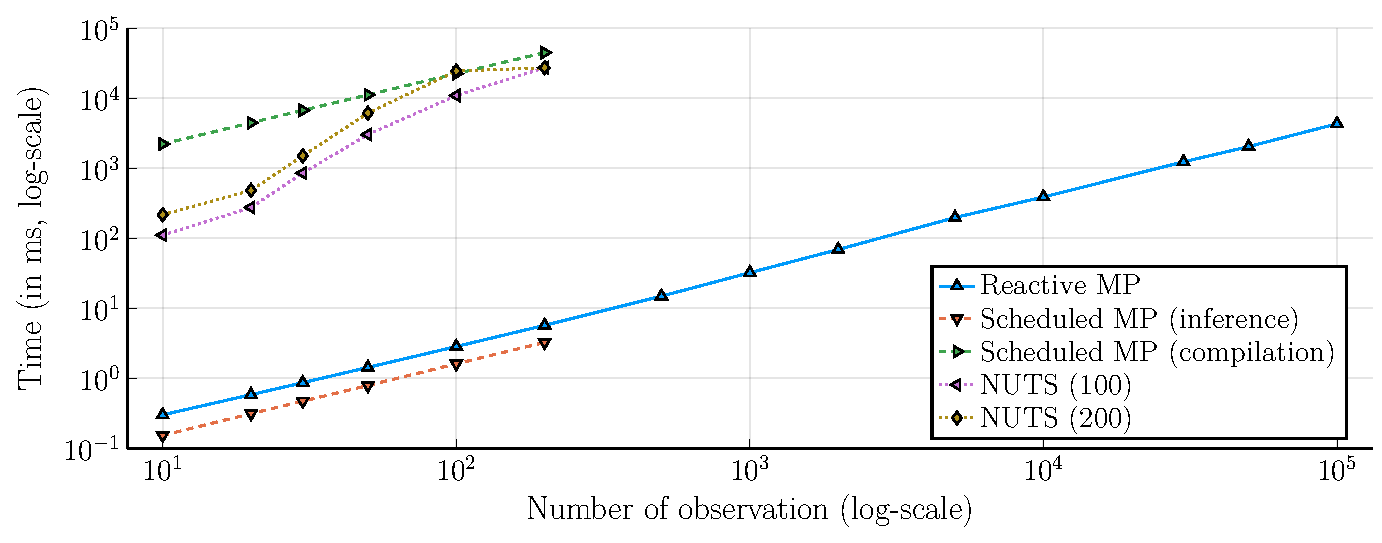
\includegraphics{contents/05-experiments/plots/lds/02-benchmark_comparison.pdf}
  }
  \caption{
    A comparison of run-time durations in milliseconds for automated Bayesian inference in the \ac{lds}~\eqref{eq:sim:lds}-\eqref{eq:sim:lds-stochastic-gaussian} with a 2-dimensional state is presented across
    different methods: reactive message passing (RxInfer), scheduled message passing (ForneyLab),
    and \ac{nuts} (Turing).
    The values in the table represent the minimum duration achieved across multiple runs.
    For RxInfer, the timings include the graph creation time.
    The ForneyLab pipeline involves model compilation followed by the execution of the inference
    procedure.
    Turing employs \ac{nuts} sampling with $100$ and $200$ samples, respectively.
    We provide benchmark results for over $300$ observations exclusively for the RxInfer
    framework.
  }
  \label{fig:sim:lds_performance_comparison}
\end{figure}

\begin{table}
  \centering
  \begin{tabular}{ |l||r|r|r|r|r|r|  }
    \hline
                    & \multicolumn{6}{|c|}{Number of observations}                                                                   \\
    \hline
                    & \multicolumn{3}{|c|}{2-dimensional}          & \multicolumn{3}{|c|}{4-dimensional}                             \\
    \hline
                    & 50                                           & 100                                 & 200  & 50   & 100  & 200  \\
    \hline
    Message passing & 2.80                                         & 2.78                                & 2.79 & 6.65 & 6.51 & 6.50 \\
    \hline
    NUTS (100)      & 2.85                                         & 2.78                                & 2.80 & 6.66 & 6.58 & 6.50 \\
    NUTS (200)      & 2.81                                         & 2.79                                & 2.80 & 6.65 & 6.52 & 6.50 \\
    \hline
  \end{tabular}
  \caption{
    Comparison of posterior result accuracy in terms of the metric~\eqref{eq:sim:average_mse} in the \ac{lds}~\eqref{eq:sim:lds}-\eqref{eq:sim:lds-stochastic-gaussian} among different methods: message passing (RxInfer and ForneyLab) and \ac{nuts} (Turing).
    Lower values indicate better performance.
    Both RxInfer and ForneyLab employ \ac{cbfe} minimization through \ac{vmp} on the full graph.
    Turing utilizes \ac{nuts} sampling with 100 and 200 samples, respectively.
  }
  \label{table:sim:lds_accuracy_comparison_2_4}
\end{table}

\begin{figure}
  \centering
  \begin{subfigure}[t]{\textwidth}
    \centering
    \resizebox{\textwidth}{!}{
        % % Recommended preamble:
% \usetikzlibrary{arrows.meta}
% \usetikzlibrary{backgrounds}
% \usepgfplotslibrary{patchplots}
% \usepgfplotslibrary{fillbetween}
% \pgfplotsset{%
%     layers/standard/.define layer set={%
%         background,axis background,axis grid,axis ticks,axis lines,axis tick labels,pre main,main,axis descriptions,axis foreground%
%     }{
%         grid style={/pgfplots/on layer=axis grid},%
%         tick style={/pgfplots/on layer=axis ticks},%
%         axis line style={/pgfplots/on layer=axis lines},%
%         label style={/pgfplots/on layer=axis descriptions},%
%         legend style={/pgfplots/on layer=axis descriptions},%
%         title style={/pgfplots/on layer=axis descriptions},%
%         colorbar style={/pgfplots/on layer=axis descriptions},%
%         ticklabel style={/pgfplots/on layer=axis tick labels},%
%         axis background@ style={/pgfplots/on layer=axis background},%
%         3d box foreground style={/pgfplots/on layer=axis foreground},%
%     },
% }

\begin{tikzpicture}[/tikz/background rectangle/.style={fill={rgb,1:red,1.0;green,1.0;blue,1.0}, fill opacity={1.0}, draw opacity={1.0}}, show background rectangle]
\begin{axis}[point meta max={nan}, point meta min={nan}, legend cell align={left}, legend columns={2}, title={}, title style={at={{(0.5,1)}}, anchor={south}, font={{\fontsize{18 pt}{23.400000000000002 pt}\selectfont}}, color={rgb,1:red,0.0;green,0.0;blue,0.0}, draw opacity={1.0}, rotate={0.0}, align={center}}, legend style={color={rgb,1:red,0.0;green,0.0;blue,0.0}, draw opacity={1.0}, line width={1}, solid, fill={rgb,1:red,1.0;green,1.0;blue,1.0}, fill opacity={1.0}, text opacity={1.0}, font={{\fontsize{14 pt}{18.2 pt}\selectfont}}, text={rgb,1:red,0.0;green,0.0;blue,0.0}, cells={anchor={west}}, at={(0.5, 1.02)}, anchor={south}}, axis background/.style={fill={rgb,1:red,1.0;green,1.0;blue,1.0}, opacity={1.0}}, anchor={north west}, xshift={1.0mm}, yshift={-1.0mm}, width={201.2mm}, height={74.2mm}, scaled x ticks={false}, xlabel={Number of observations in dataset (log10-scale)}, x tick style={color={rgb,1:red,0.0;green,0.0;blue,0.0}, opacity={1.0}}, x tick label style={color={rgb,1:red,0.0;green,0.0;blue,0.0}, opacity={1.0}, rotate={0}}, xlabel style={at={(ticklabel cs:0.5)}, anchor=near ticklabel, at={{(ticklabel cs:0.5)}}, anchor={near ticklabel}, font={{\fontsize{16 pt}{20.8 pt}\selectfont}}, color={rgb,1:red,0.0;green,0.0;blue,0.0}, draw opacity={1.0}, rotate={0.0}}, xmode={log}, log basis x={10}, xmajorgrids={true}, xmin={7.585775750291836}, xmax={131825.67385564075}, xticklabels={{$10^1$,$10^2$,$10^3$,$10^4$,$10^5$}}, xtick={{10,100,1000,10000,100000}}, xtick align={inside}, xticklabel style={font={{\fontsize{14 pt}{18.2 pt}\selectfont}}, color={rgb,1:red,0.0;green,0.0;blue,0.0}, draw opacity={1.0}, rotate={0.0}}, x grid style={color={rgb,1:red,0.0;green,0.0;blue,0.0}, draw opacity={0.1}, line width={0.5}, solid}, axis x line*={left}, x axis line style={color={rgb,1:red,0.0;green,0.0;blue,0.0}, draw opacity={1.0}, line width={1}, solid}, scaled y ticks={false}, ylabel={Time (in ms, log10-scale)}, y tick style={color={rgb,1:red,0.0;green,0.0;blue,0.0}, opacity={1.0}}, y tick label style={color={rgb,1:red,0.0;green,0.0;blue,0.0}, opacity={1.0}, rotate={0}}, ylabel style={at={(ticklabel cs:0.5)}, anchor=near ticklabel, at={{(ticklabel cs:0.5)}}, anchor={near ticklabel}, font={{\fontsize{16 pt}{20.8 pt}\selectfont}}, color={rgb,1:red,0.0;green,0.0;blue,0.0}, draw opacity={1.0}, rotate={0.0}}, ymode={log}, log basis y={10}, ymajorgrids={true}, ymin={0.1}, ymax={10000.0}, yticklabels={{$10^{-1}$,$10^{0}$,$10^{1}$,$10^{2}$,$10^{3}$,$10^{4}$}}, ytick={{0.1,1.0,10.0,100.0,1000.0,10000.0}}, ytick align={inside}, yticklabel style={font={{\fontsize{14 pt}{18.2 pt}\selectfont}}, color={rgb,1:red,0.0;green,0.0;blue,0.0}, draw opacity={1.0}, rotate={0.0}}, y grid style={color={rgb,1:red,0.0;green,0.0;blue,0.0}, draw opacity={0.1}, line width={0.5}, solid}, axis y line*={left}, y axis line style={color={rgb,1:red,0.0;green,0.0;blue,0.0}, draw opacity={1.0}, line width={1}, solid}, colorbar={false}]
    \addplot[color={rgb,1:red,0.3059;green,0.4745;blue,0.6549}, name path={e3a778d4-6418-4761-9fbc-ca4904cba719}, draw opacity={1.0}, line width={1}, solid, mark={diamond*}, mark size={3.0 pt}, mark repeat={1}, mark options={color={rgb,1:red,0.0;green,0.0;blue,0.0}, draw opacity={1.0}, fill={rgb,1:red,0.3059;green,0.4745;blue,0.6549}, fill opacity={1.0}, line width={0.75}, rotate={0}, solid}]
        table[row sep={\\}]
        {
            \\
            10.0  0.2931  \\
            20.0  0.5694  \\
            30.0  0.8533  \\
            50.0  1.4012  \\
            100.0  2.7853  \\
            200.0  5.6427  \\
            500.0  14.7833  \\
            1000.0  32.3217  \\
            2000.0  69.8363  \\
            5000.0  179.132  \\
            10000.0  377.7713  \\
            30000.0  1202.7147  \\
            50000.0  2038.2433  \\
            100000.0  4131.1598  \\
        }
        ;
    \addlegendentry {2 dimensional}
    \addplot[color={rgb,1:red,0.949;green,0.5569;blue,0.1686}, name path={e49bc6b2-00dd-4959-92f9-1db3bab8c102}, draw opacity={1.0}, line width={1}, dashed, mark={*}, mark size={3.0 pt}, mark repeat={1}, mark options={color={rgb,1:red,0.0;green,0.0;blue,0.0}, draw opacity={1.0}, fill={rgb,1:red,0.949;green,0.5569;blue,0.1686}, fill opacity={1.0}, line width={0.75}, rotate={0}, solid}]
        table[row sep={\\}]
        {
            \\
            10.0  0.2994  \\
            20.0  0.5814  \\
            30.0  0.8625  \\
            50.0  1.4243  \\
            100.0  2.8341  \\
            200.0  5.6979  \\
            500.0  14.8631  \\
            1000.0  32.2077  \\
            2000.0  69.0191  \\
            5000.0  197.8437  \\
            10000.0  388.9888  \\
            30000.0  1236.1908  \\
            50000.0  2044.8108  \\
            100000.0  4327.0868  \\
        }
        ;
    \addlegendentry {4 dimensional}
    \addplot[color={rgb,1:red,0.8824;green,0.3412;blue,0.349}, name path={d4bd6730-897d-4bb8-941f-c9226874147a}, draw opacity={1.0}, line width={1}, dotted, mark={square*}, mark size={3.0 pt}, mark repeat={1}, mark options={color={rgb,1:red,0.0;green,0.0;blue,0.0}, draw opacity={1.0}, fill={rgb,1:red,0.8824;green,0.3412;blue,0.349}, fill opacity={1.0}, line width={0.75}, rotate={0}, solid}]
        table[row sep={\\}]
        {
            \\
            10.0  0.3171  \\
            20.0  0.615  \\
            30.0  0.9157  \\
            50.0  1.5115  \\
            100.0  3.0052  \\
            200.0  6.0854  \\
            500.0  15.9601  \\
            1000.0  34.4974  \\
            2000.0  74.1862  \\
            5000.0  202.8761  \\
            10000.0  412.2831  \\
            30000.0  1327.4848  \\
            50000.0  2164.303  \\
            100000.0  4472.756  \\
        }
        ;
    \addlegendentry {8 dimensional}
    \addplot[color={rgb,1:red,0.4627;green,0.7176;blue,0.698}, name path={71e972a8-1a88-40e6-862d-a1d49a6be8c2}, draw opacity={1.0}, line width={1}, dashdotted, mark={triangle*}, mark size={3.0 pt}, mark repeat={1}, mark options={color={rgb,1:red,0.0;green,0.0;blue,0.0}, draw opacity={1.0}, fill={rgb,1:red,0.4627;green,0.7176;blue,0.698}, fill opacity={1.0}, line width={0.75}, rotate={0}, solid}]
        table[row sep={\\}]
        {
            \\
            10.0  0.4773  \\
            20.0  0.9561  \\
            30.0  1.4435  \\
            50.0  2.3992  \\
            100.0  4.7535  \\
            200.0  9.8103  \\
            500.0  25.7334  \\
            1000.0  53.8492  \\
            2000.0  111.9562  \\
            5000.0  300.5951  \\
            10000.0  579.3586  \\
            30000.0  1872.9722  \\
            50000.0  3063.1097  \\
            100000.0  6285.8989  \\
        }
        ;
    \addlegendentry {16 dimensional}
\end{axis}
\end{tikzpicture}

        \includegraphics{contents/05-experiments/plots/lds/02-rxinfer_rotating_scalability_size.pdf}
    }
    \caption{Scalability benchmark across different dimensionalities of the state vector with respect to the number of observations in the dataset.
    }
    \label{fig:sim:lds_scalability_size}
  \end{subfigure}
  \hfill
  \begin{subfigure}[t]{\textwidth}
    \centering
    \resizebox{\textwidth}{!}{
        % % Recommended preamble:
% \usetikzlibrary{arrows.meta}
% \usetikzlibrary{backgrounds}
% \usepgfplotslibrary{patchplots}
% \usepgfplotslibrary{fillbetween}
% \pgfplotsset{%
%     layers/standard/.define layer set={%
%         background,axis background,axis grid,axis ticks,axis lines,axis tick labels,pre main,main,axis descriptions,axis foreground%
%     }{
%         grid style={/pgfplots/on layer=axis grid},%
%         tick style={/pgfplots/on layer=axis ticks},%
%         axis line style={/pgfplots/on layer=axis lines},%
%         label style={/pgfplots/on layer=axis descriptions},%
%         legend style={/pgfplots/on layer=axis descriptions},%
%         title style={/pgfplots/on layer=axis descriptions},%
%         colorbar style={/pgfplots/on layer=axis descriptions},%
%         ticklabel style={/pgfplots/on layer=axis tick labels},%
%         axis background@ style={/pgfplots/on layer=axis background},%
%         3d box foreground style={/pgfplots/on layer=axis foreground},%
%     },
% }

\begin{tikzpicture}[/tikz/background rectangle/.style={fill={rgb,1:red,1.0;green,1.0;blue,1.0}, fill opacity={1.0}, draw opacity={1.0}}, show background rectangle]
\begin{axis}[point meta max={nan}, point meta min={nan}, legend cell align={left}, legend columns={1}, title={}, title style={at={{(0.5,1)}}, anchor={south}, font={{\fontsize{18 pt}{23.400000000000002 pt}\selectfont}}, color={rgb,1:red,0.0;green,0.0;blue,0.0}, draw opacity={1.0}, rotate={0.0}, align={center}}, legend style={color={rgb,1:red,0.0;green,0.0;blue,0.0}, draw opacity={1.0}, line width={1}, solid, fill={rgb,1:red,1.0;green,1.0;blue,1.0}, fill opacity={1.0}, text opacity={1.0}, font={{\fontsize{14 pt}{18.2 pt}\selectfont}}, text={rgb,1:red,0.0;green,0.0;blue,0.0}, cells={anchor={west}}, at={(1.02, 0.5)}, anchor={west}}, axis background/.style={fill={rgb,1:red,1.0;green,1.0;blue,1.0}, opacity={1.0}}, anchor={north west}, xshift={1.0mm}, yshift={-1.0mm}, width={196.2mm}, height={74.2mm}, scaled x ticks={false}, xlabel={Number of dimensions}, x tick style={color={rgb,1:red,0.0;green,0.0;blue,0.0}, opacity={1.0}}, x tick label style={color={rgb,1:red,0.0;green,0.0;blue,0.0}, opacity={1.0}, rotate={0}}, xlabel style={at={(ticklabel cs:0.5)}, anchor=near ticklabel, at={{(ticklabel cs:0.5)}}, anchor={near ticklabel}, font={{\fontsize{16 pt}{20.8 pt}\selectfont}}, color={rgb,1:red,0.0;green,0.0;blue,0.0}, draw opacity={1.0}, rotate={0.0}}, xmajorgrids={true}, xmin={1.58}, xmax={16.42}, xticklabels={{2,4,8,16}}, xtick={{2,4,8,16}}, xtick align={inside}, xticklabel style={font={{\fontsize{14 pt}{18.2 pt}\selectfont}}, color={rgb,1:red,0.0;green,0.0;blue,0.0}, draw opacity={1.0}, rotate={0.0}}, x grid style={color={rgb,1:red,0.0;green,0.0;blue,0.0}, draw opacity={0.1}, line width={0.5}, solid}, axis x line*={left}, x axis line style={color={rgb,1:red,0.0;green,0.0;blue,0.0}, draw opacity={1.0}, line width={1}, solid}, scaled y ticks={false}, ylabel={Time (in ms, log10-scale)}, y tick style={color={rgb,1:red,0.0;green,0.0;blue,0.0}, opacity={1.0}}, y tick label style={color={rgb,1:red,0.0;green,0.0;blue,0.0}, opacity={1.0}, rotate={0}}, ylabel style={at={(ticklabel cs:0.5)}, anchor=near ticklabel, at={{(ticklabel cs:0.5)}}, anchor={near ticklabel}, font={{\fontsize{16 pt}{20.8 pt}\selectfont}}, color={rgb,1:red,0.0;green,0.0;blue,0.0}, draw opacity={1.0}, rotate={0.0}}, ymode={log}, log basis y={10}, ymajorgrids={true}, ymin={0.1}, ymax={10000.0}, yticklabels={{$10^{-1}$,$10^{0}$,$10^{1}$,$10^{2}$,$10^{3}$,$10^{4}$}}, ytick={{0.1,1.0,10.0,100.0,1000.0,10000.0}}, ytick align={inside}, yticklabel style={font={{\fontsize{14 pt}{18.2 pt}\selectfont}}, color={rgb,1:red,0.0;green,0.0;blue,0.0}, draw opacity={1.0}, rotate={0.0}}, y grid style={color={rgb,1:red,0.0;green,0.0;blue,0.0}, draw opacity={0.1}, line width={0.5}, solid}, axis y line*={left}, y axis line style={color={rgb,1:red,0.0;green,0.0;blue,0.0}, draw opacity={1.0}, line width={1}, solid}, colorbar={false}]
    \addplot[color={rgb,1:red,0.3059;green,0.4745;blue,0.6549}, name path={a51e7468-e62c-4398-99ec-1b4cef59b1de}, draw opacity={1.0}, line width={1}, solid, mark={triangle*}, mark size={3.0 pt}, mark repeat={1}, mark options={color={rgb,1:red,0.0;green,0.0;blue,0.0}, draw opacity={1.0}, fill={rgb,1:red,0.3059;green,0.4745;blue,0.6549}, fill opacity={1.0}, line width={0.75}, rotate={0}, solid}]
        table[row sep={\\}]
        {
            \\
            2.0  0.2931  \\
            4.0  0.2994  \\
            8.0  0.3171  \\
            16.0  0.4773  \\
        }
        ;
    \addlegendentry {Reactive MP inference (10 observations)}
    \addplot[color={rgb,1:red,0.949;green,0.5569;blue,0.1686}, name path={ca5e1e4c-08d6-4d6a-9d55-9fb34d26d8ac}, draw opacity={1.0}, line width={1}, dashed, mark={triangle*}, mark size={3.0 pt}, mark repeat={1}, mark options={color={rgb,1:red,0.0;green,0.0;blue,0.0}, draw opacity={1.0}, fill={rgb,1:red,0.949;green,0.5569;blue,0.1686}, fill opacity={1.0}, line width={0.75}, rotate={180}, solid}]
        table[row sep={\\}]
        {
            \\
            2.0  32.3217  \\
            4.0  32.2077  \\
            8.0  34.4974  \\
            16.0  53.8492  \\
        }
        ;
    \addlegendentry {Reactive MP inference (1000 observations)}
    \addplot[color={rgb,1:red,0.8824;green,0.3412;blue,0.349}, name path={8c2f9457-3d7f-4552-bb01-ec5beeeb87ad}, draw opacity={1.0}, line width={1}, dotted, mark={triangle*}, mark size={3.0 pt}, mark repeat={1}, mark options={color={rgb,1:red,0.0;green,0.0;blue,0.0}, draw opacity={1.0}, fill={rgb,1:red,0.8824;green,0.3412;blue,0.349}, fill opacity={1.0}, line width={0.75}, rotate={270}, solid}]
        table[row sep={\\}]
        {
            \\
            2.0  377.7713  \\
            4.0  388.9888  \\
            8.0  412.2831  \\
            16.0  579.3586  \\
        }
        ;
    \addlegendentry {Reactive MP inference (10000 observations)}
    \addplot[color={rgb,1:red,0.4627;green,0.7176;blue,0.698}, name path={88323c08-2b3f-43b3-a41f-4b181db02a91}, draw opacity={1.0}, line width={1}, dashdotted, mark={triangle*}, mark size={3.0 pt}, mark repeat={1}, mark options={color={rgb,1:red,0.0;green,0.0;blue,0.0}, draw opacity={1.0}, fill={rgb,1:red,0.4627;green,0.7176;blue,0.698}, fill opacity={1.0}, line width={0.75}, rotate={90}, solid}]
        table[row sep={\\}]
        {
            \\
            2.0  4131.1598  \\
            4.0  4327.0868  \\
            8.0  4472.756  \\
            16.0  6285.8989  \\
        }
        ;
    \addlegendentry {Reactive MP inference (100000 observations)}
\end{axis}
\end{tikzpicture}

        \includegraphics{contents/05-experiments/plots/lds/02-rxinfer_rotating_scalability_dims.pdf}
    }
    \caption{Scalability benchmark across different numbers of observations in the dataset with respect to the dimensionality of the state vector.}
    \label{fig:sim:lds_scalability_dims}
  \end{subfigure}
  \hfill \caption{
    Benchmark results of automated Bayesian inference for the \ac{lds}~\eqref{eq:sim:lds}-\eqref{eq:sim:lds-stochastic-gaussian} using the RxInfer framework.
    The results illustrate the excellent scalability of the RxInfer framework for varying numbers
    of observations in the dataset and different dimensionalities of the state vector.
    The values in the table represent the minimum duration observed across multiple runs,
    including graph creation time.
  }
  \label{fig:sim:lds_scalability}
\end{figure}

This section demonstrates the scalability and run-time efficiency characteristics of the proposed \ac{rmp} architecture for the \ac{lds}~\eqref{eq:sim:lds}-\eqref{eq:sim:lds-stochastic-gaussian} compare to other methods.
The main benchmark results, which highlight the performance and scalability of the RxInfer
framework, are presented in Figure~\ref{fig:sim:lds_performance_comparison}.
The benchmark analysis reveals that the RxInfer framework achieves superior performance and
scalability compared to the alternative packages when considering both model creation and
inference execution.
It outperforms the packages compared in terms of time and memory consumption\footnote{Not
  present in the table.
}, indicating its
efficiency in handling the inference task \footnote{Detailed benchmark results,
  including comprehensive evaluations and comparisons of the RxInfer framework with ForneyLab
  and Turing across various experimental scenarios, can be found at
  \url{https://github.com/bvdmitri/phdthesis/tree/main/experiments}.
}.
Moreover, the RxInfer framework demonstrates its ability to handle large-scale models
consisting of hundreds of thousands of variables (\hyperlink{experiments:scalability}{\emph{Scalability}}).
This scalability is depicted in Figure~\ref{fig:sim:lds_scalability}, illustrating the
framework's ability to efficiently tackle complex Bayesian inference tasks involving
high-dimensional data.

Figure~\ref{fig:sim:lds_performance_comparison} reveals an interesting finding: the ForneyLab
package demonstrates faster execution of the inference task for this specific model compared
to the RxInfer framework.
This is attributed to ForneyLab's thorough analysis of the \ac{tffg} during precompilation,
enabling the creation of an efficient predefined message update schedule in advance.
As a result, the inference procedure is executed more efficiently.
However, it is important to note that ForneyLab's schedule-based approach suffers from
prolonged latencies in the graph creation and precompilation stages, as discussed in
Section~\ref{chapter-01:section:motivation}.
These stages experience high compilation times, and any modification in the model
specification requires complete recompilation.
This limitation restricts the exploration of "what-if" scenarios in the model specification
space and does not support online model structure adaptation, hindering the flexibility of the
scheduled message passing-based approaches.
In contrast, RxInfer adopts a dynamic approach by creating and executing the reactive message
passing scheme without relying on full graph analysis and naturally supports online model adaptation
in its core design.
This feature incurs certain run-time performance costs due to the additional management of reactive dependencies within the graph
during the inference process.
Despite these costs, RxInfer offers the advantage of adaptability and flexibility,
particularly when dealing with models of significant size and complexity.

The execution times of the \ac{nuts} algorithm, implemented in the Turing package, are mainly based
on the number of samples employed in the sampling procedure.
Generally, in sampling-based packages, a higher number of samples yields improved
approximations at the cost of longer computation times.
Determining an optimal number of samples is a nontrivial task, as it necessitates
consideration of the specific model and available dataset, as well as careful post-analysis of
the results.
For this experiment, the number of samples was manually selected to ensure that the
\ac{nuts} estimates of the corresponding posteriors exhibit precision comparable to the
message passing-based methods, as evaluated using the accuracy
metric~\eqref{eq:sim:average_mse}.
However, it should be noted that the sampling-based approach exhibits poor scalability when
confronted with a large number of latent states in a \ac{lds}, especially when the number of samples is large.
Consequently, its viability for real-time applications in the field is practically impossible.

We specifically focus on presenting benchmark results for a large number of observations using
the RxInfer framework, as executing the inference process with the alternative frameworks would
require significantly longer computation times, which are not suitable for real-time
applications.
To illustrate, Figure~\ref{fig:sim:lds_model_graph} provides an estimate that a static
dataset with $100,000$ observations results in a corresponding \ac{tffg}
for this model with approximately $700,000$ nodes.
RxInfer completes the inference task on a full model graph for such a size in less than ten
seconds, corresponding to less than $0.1$ milliseconds per observation (\hyperlink{experiments:efficiency}{\emph{Run-time efficiency and speed}}).
This result highlights the efficiency and scalability of the RxInfer framework.

In addition to performance and scalability, the accuracy of the estimated posteriors is a
critical factor in Bayesian inference.
Table~\ref{table:sim:lds_accuracy_comparison_2_4} presents the accuracy results in terms of
the \ac{ae} metric~\eqref{eq:sim:average_mse}.
It is observed that all methods yield comparable accuracy in estimating posteriors.
The scalability analysis for this type of model demonstrates that RxInfer can efficiently and
accurately perform inferences on this type of model (\hyperlink{experiments:accuracy}{\emph{Posterior accuracy}}).
This makes the \ac{rmp} framework, and RxInfer in particular, a better choice for real-world
applications involving high-dimensional data and linear dependencies among states.

In the subsequent section, we delve into running more difficult inference tasks in nonlinear
dynamical systems that share a similar structure to an \ac{lds} but entail more complex non-conjugate
relationships between variables.

